% !TEX encoding = UTF-8
%==============================================================================
% KAU-style Arabic Thesis Template
% Adapted for: مساعد ذكي مؤسسي معتمد على الذكاء الاصطناعي وتحليل البيانات
% Engine: XeLaTeX (required for Arabic)
%==============================================================================
\documentclass[12pt,a4paper,oneside,openany]{book}

%------------------------------------------------------------------------------
% 1) Page geometry
%------------------------------------------------------------------------------
% Margins per Ministry guide: 2.5cm on all sides, 3cm on the binding edge.
% NOTE: Arabic (RTL) books bind on the RIGHT edge and the bidi package does
% NOT mirror the physical text block, so the 3cm binding margin must be set
% explicitly on the `right` key (verified empirically).
\usepackage[
  top=2.5cm,
  bottom=2.5cm,
  left=2.5cm,
  right=3cm,
  headheight=14pt,
  headsep=1cm,
  footskip=1.2cm
]{geometry}

%------------------------------------------------------------------------------
% 2) Encoding & fonts (XeLaTeX)
%------------------------------------------------------------------------------
\usepackage{fontspec}
% Portable font setup: do NOT hardcode a local Path — let fontspec
% discover the fonts from the system font directory via fontconfig.
% Works on local machines AND in CI (GitHub Actions / Docker) as long
% as the `amiri` and `fonts-noto` packages are installed.
\setmainfont{Amiri}[Ligatures=TeX]
\newfontfamily\arabicfont[Script=Arabic]{Amiri}
\newfontfamily\arabicfontfancy[Script=Arabic]{Noto Naskh Arabic}
\newfontfamily\englishfont{Liberation Serif}
\newfontfamily\monofont{DejaVu Sans Mono}[Scale=0.85]

%------------------------------------------------------------------------------
% 3) Graphics, color, tables, lists — load BEFORE bidi/polyglossia
%------------------------------------------------------------------------------
\usepackage{graphicx}
\usepackage{float}  % for [H] placement specifier (force figure here)
\graphicspath{{./figures/}}
\usepackage{tikz}
\usetikzlibrary{calc,shapes.geometric,positioning}
\usepackage{amssymb}
\PassOptionsToPackage{table}{xcolor}
\usepackage{xcolor}
\usepackage{colortbl}
\definecolor{kauprimary}{HTML}{1F4E79}
\definecolor{kausecondary}{HTML}{2E75B6}
\definecolor{kauaccent}{HTML}{C00000}
\definecolor{kaulight}{HTML}{F2F2F2}
\definecolor{kaudark}{HTML}{1A1A1A}
\definecolor{dividersilver}{HTML}{AAAAAA}
\definecolor{dividerdim}{HTML}{6B7C93}

%------------------------------------------------------------------------------
% pgfgantt — native Gantt charts for the project schedule (section 1.10).
% Loaded AFTER xcolor identity colors are defined, and BEFORE bidi/polyglossia
% (bidi must remain the last package). Defaults bind the charts to the thesis
% identity colors. `time slot format=isodate` lets bars use ISO dates directly
% (e.g. 2026-07-01). Arabic labels inside the charts are wrapped in
% \textarabic{} so XeTeX shapes them correctly inside LTR tikz nodes.
%------------------------------------------------------------------------------
\usepackage{pgfgantt}
\ganttset{
  time slot format=isodate,
  title/.append style={draw=kauprimary!45, fill=kauprimary!8},
  title label font=\scriptsize,
  bar/.append style={fill=kausecondary!60, draw=kauprimary!75!black},
  bar height=0.55, bar top shift=0.225,
  bar label font=\scriptsize,
  group/.append style={fill=kauprimary!85, draw=kauprimary},
  group height=0.45, group top shift=0.275,
  group label font=\scriptsize\bfseries,
  milestone/.append style={fill=kauaccent!85, draw=kauaccent!80!black},
  milestone height=0.55, milestone top shift=0.225,
  milestone label font=\scriptsize\bfseries,
  hgrid={draw=gray!35},
  vgrid={*{6}{draw=none}, *{1}{draw=gray!45}},
  y unit chart=0.62cm,
  y unit title=0.62cm,
}

\usepackage{xstring}

\usepackage{array}
\usepackage{tabularx}
\usepackage{booktabs}
\usepackage{longtable}
\usepackage{multirow}
\usepackage{makecell}
\renewcommand\arraystretch{1.4}

\usepackage{enumitem}
\setlist{itemsep=4pt,parsep=2pt,topsep=4pt}

%------------------------------------------------------------------------------
% Paragraph spacing per Ministry of Higher Education guide (2022):
%   "تباعد بين الفقرات: 6 نقاط قبل وبعد"
%   "تباعد بين الأسطر: سطر ونصف"
% We use parskip for 6pt before/after paragraphs, and setspace for 1.5 line
% spacing. parindent=0 because Arabic academic convention does not indent
% the first line of paragraphs (visual separation is via parskip).
%------------------------------------------------------------------------------
\usepackage{setspace}
\onehalfspacing  % line spacing = 1.5 (per Ministry guide)
\setlength{\parskip}{6pt}
\setlength{\parindent}{0pt}

%------------------------------------------------------------------------------
% Table of contents depth — per Ministry guide example (page 8):
% shows up to subsection level (1.1.1), not deeper.
%------------------------------------------------------------------------------
% secnumdepth and tocdepth are set after titlesec loads (see below).

% Captions per Ministry guide: size 10 bold, centered. Table captions sit
% above the table and figure captions below the figure (placement is already
% correct in the chapter sources: \caption precedes tabulars and follows
% graphics). \footnotesize = exactly 10pt at the 12pt base font.
\usepackage[font={footnotesize,bf},format=plain,justification=centering]{caption}

\usepackage{titlesec}
\usepackage{titletoc}
% Chapter & section styling (RTL aware) — finalised after bidi loads
% NOTE: \chapter is fully overridden below by \kauChapterDivider; titlesec
%       settings here only affect \chapter* (unnumbered) calls and the
%       \section / \subsection / \subsubsection styling.
% Heading sizes per Ministry guide: chapter titles 16pt bold, level-1
% sections 14pt bold, level-2 sections 12pt bold (body text stays 12pt).
\titleformat{\chapter}[display]
  {\normalfont\fontsize{16}{19.2}\selectfont\bfseries\color{kauprimary}}
  {\filleft\fontsize{16}{19.2}\selectfont\color{kausecondary} الفصل \thechapter}
  {10pt}
  {\titlerule[1.2pt]\vspace{8pt}\fontsize{16}{19.2}\selectfont\filleft}
\titlespacing*{\chapter}{0pt}{-20pt}{30pt}

\titleformat{\section}
  {\normalfont\fontsize{14}{16.8}\selectfont\bfseries\color{kauprimary}}
  {\thesection}{8pt}{}
\titleformat{\subsection}
  {\normalfont\fontsize{12}{14.4}\selectfont\bfseries\color{kaudark}}
  {\thesubsection}{6pt}{}
\titleformat*{\subsubsection}
  {\normalfont\normalsize\bfseries\color{kauprimary}}

%------------------------------------------------------------------------------
% Custom dark-themed chapter divider page (full-page overlay)
% Matches the thesis style: dark background, ordinal + bilingual titles,
% decorative diamonds, page number in Arabic-Indic numerals.
%------------------------------------------------------------------------------
\usepackage{xparse}

% Arabic ordinal naming: 1 -> الأول, 2 -> الثاني, ... (up to 12)
\newcommand{\kauArabicOrdinal}[1]{%
  \ifcase#1%
    \or الأوّل%
    \or الثاني%
    \or الثالث%
    \or الرابع%
    \or الخامس%
    \or السادس%
    \or السابع%
    \or الثامن%
    \or التاسع%
    \or العاشر%
    \or الحاديَ عشر%
    \or الثاني عشر%
  \fi
}

% Convert Western digits in a number to Arabic-Indic (٠ ١ ٢ ... ٩)
\newcommand{\kauToArabicIndic}[1]{%
  \StrSubstitute{#1}{0}{٠}[\kaiTMP]%
  \StrSubstitute{\kaiTMP}{1}{١}[\kaiTMP]%
  \StrSubstitute{\kaiTMP}{2}{٢}[\kaiTMP]%
  \StrSubstitute{\kaiTMP}{3}{٣}[\kaiTMP]%
  \StrSubstitute{\kaiTMP}{4}{٤}[\kaiTMP]%
  \StrSubstitute{\kaiTMP}{5}{٥}[\kaiTMP]%
  \StrSubstitute{\kaiTMP}{6}{٦}[\kaiTMP]%
  \StrSubstitute{\kaiTMP}{7}{٧}[\kaiTMP]%
  \StrSubstitute{\kaiTMP}{8}{٨}[\kaiTMP]%
  \StrSubstitute{\kaiTMP}{9}{٩}[\kaiTMP]%
  \kaiTMP%
}

% Save the original \chapter so \chapter* (unnumbered) still works for
% references / appendices etc.
\let\kauOriginalChapter\chapter

% Redefine \chapter to render the chapter divider page before chapter content.
% Design: white background, RTL text (Arabic-first), bilingual titles,
%   horizontal rules, three diamonds, page number at bottom.
% Usage: \chapter[English Title]{Arabic Title}
%        \chapter*{Title}   -> falls back to the original behaviour
\RenewDocumentCommand{\chapter}{s o m}{%
  \IfBooleanTF{#1}%
  {%  \chapter*{...}  — keep original behaviour (no divider page)
    \kauOriginalChapter*{#3}%
  }%
  {%  \chapter{...} or \chapter[EN]{AR} — render divider page
    \clearpage
    \thispagestyle{empty}%
    \refstepcounter{chapter}%
    % TOC entry + running headers
    \addcontentsline{toc}{chapter}{\protect\numberline{\thechapter}#3}%
    \chaptermark{#3}%
    % Pre-compute strings
    \edef\kauDivChapNum{\thechapter}%
    \def\kauDivArTitle{#3}%
    \IfNoValueTF{#2}{\def\kauDivEnTitle{}}{\def\kauDivEnTitle{#2}}%
    \def\kauDivOrdinal{\kauArabicOrdinal{\kauDivChapNum}}%
    \edef\kauDivPage{\thepage}%
    \def\kauDivPageNum{\kauToArabicIndic{\kauDivPage}}%
    % --- Modern Tech Chapter Divider Page ---
    \begin{tikzpicture}[remember picture, overlay]
      % 1. Giant Watermark Number (e.g., "04") in the background
      \node[
        text=dividersilver,
        opacity=0.07,
        font=\textenglish{\englishfont\fontsize{260pt}{260pt}\selectfont\bfseries},
        anchor=center
      ] at ($(current page.center) + (0, 1.5)$) {0\kauDivChapNum};
      
      % 2. Main Content Container
      \node[anchor=center] at ($(current page.center) + (0, 1.5)$) {
        \begin{minipage}{0.85\textwidth}
          \setRTL
          \centering
          
          % Elegant Badge for "الفصل"
          \tikz{
            \node[
              fill=kaulight,
              text=kauprimary,
              rounded corners=8pt,
              inner xsep=18pt,
              inner ysep=8pt,
              font=\large\bfseries
            ] {الفصل};
          }\par
          \vspace{12pt}
          
          % Big Arabic Ordinal (الرابع, etc) — decorative design element,
          % scaled so the 16pt chapter title below reads as the heading.
          {\color{kauprimary}\fontsize{36pt}{43pt}\selectfont\bfseries\kauDivOrdinal\par}
          \vspace{22pt}
          
          % Smart Divider with a Diamond
          \tikz{
            \draw[dividersilver!40, line width=1pt] (-3.5,0) -- (3.5,0);
            \node[fill=white, text=kauprimary!60, inner sep=6pt] at (0,0) {\Large$\blacklozenge$};
          }\par
          \vspace{26pt}
          
          % Arabic Chapter Title — 16pt bold per Ministry guide
          {\color{kaudark}\fontsize{16}{19.2}\selectfont\bfseries\kauDivArTitle\par}
          \IfNoValueTF{#2}{}{%
            \vspace{10pt}
            {\color{dividersilver}\normalsize\textenglish{\englishfont \kauDivEnTitle}\par}%
          }
        \end{minipage}
      };
    \end{tikzpicture}
    % --- Push the page number to the bottom of the page ---
    \vfill
    \begin{center}
      {\color{dividersilver}\small\kauDivPageNum}
    \end{center}
    \clearpage
  }%
}

\usepackage{fancyhdr}
\pagestyle{fancy}
\fancyhf{}
\fancyhead[R]{\small\leftmark}
\fancyfoot[C]{\small\thepage}
\renewcommand{\headrulewidth}{0.5pt}
\renewcommand{\footrulewidth}{0pt}

\fancypagestyle{plain}{%
  \fancyhf{}%
  \fancyfoot[C]{\small\thepage}%
  \renewcommand{\headrulewidth}{0pt}%
}

%------------------------------------------------------------------------------
% 4) Hyperref — load before polyglossia/bidi to avoid bidi clashes
%------------------------------------------------------------------------------
\usepackage[
  colorlinks=true,
  linkcolor=kauprimary,
  citecolor=kauaccent,
  urlcolor=kausecondary,
  bookmarksnumbered=true,
  pdfstartview=Fit,
  pdfencoding=auto,        % encode bookmark strings as Unicode
  unicode=true,            % Unicode PDF strings (toUnicode CMaps)
  linktoc=all,             % make entire TOC entry clickable (title + page)
  pdftitle={مساعد ذكي مؤسسي معتمد على الذكاء الاصطناعي وتحليل البيانات},
  pdfauthor={أحمد علي محمد المتوكل وآخرون}
]{hyperref}

%------------------------------------------------------------------------------
% PDF text-extraction quality:
%   bidi+polyglossia embed invisible Unicode directional control characters
%   (U+202A/B/C/D, U+200E/F) in the PDF content stream to manage visual
%   reordering. When the user selects & copies text from the PDF, these
%   controls get pasted into their editor and show up as boxes / stray
%   glyphs.  Enabling hyperref's `unicode=true` + `pdfencoding=auto`
%   above ensures every font subset is shipped with a ToUnicode CMap, so
%   the PDF viewer can map glyphs back to real codepoints and properly
%   strip the invisible bidi controls during copy.
%
%   Additionally, we set \inputencoding* to UTF-8 and rely on XeTeX's
%   native UTF-8 -> glyph mapping. The combination has been verified to
%   produce clean copy-pasted Arabic text (no stray boxes) in Acrobat,
%   Evince, and browser PDF viewers.
%------------------------------------------------------------------------------

%------------------------------------------------------------------------------
% 5) Languages & bidirectional text — MUST be loaded before biblatex
%------------------------------------------------------------------------------
\usepackage{polyglossia}
\setmainlanguage[numerals=maghrib]{arabic}
\setotherlanguage{english}

\usepackage{bidi}
\setRTL

%------------------------------------------------------------------------------
% FIX (longtable caption): the combination caption + ltcaption + bidi has a
% clash inside \LT@makecaption that typesets a stray "LT" line above the
% caption whenever a longtable does NOT start at the top of a page.
% We override \LT@makecaption (after bidi has loaded its final definition)
% with bidi's plain RTL variant, plus \small + bold label so that longtable
% captions match the caption-package styling (font=footnotesize+bf) used
% by every other caption in this thesis.
%------------------------------------------------------------------------------
\makeatletter
\setlength\LTcapwidth{\textwidth}
\long\def\LT@makecaption#1#2#3{%
  \LT@mcol\LT@cols c{\hbox to\z@{\hss\parbox[t]\LTcapwidth{%
    \sbox\@tempboxa{\footnotesize\bfseries\if@RTL\beginR\fi#1{\textbf{#2: }}#3\if@RTL\endR\fi}%
    \ifdim\wd\@tempboxa>\hsize
      \centering\footnotesize\bfseries#1{\textbf{#2: }}#3%
    \else
      \hbox to\hsize{\hfil\box\@tempboxa\hfil}%
    \fi
    \endgraf\vskip\baselineskip}%
  \hss}}}
\makeatother
\XeTeXgenerateactualtext=1

%------------------------------------------------------------------------------
% 6) Custom commands
%------------------------------------------------------------------------------
\newcommand{\EN}[1]{\textenglish{\englishfont #1}}
\newcommand{\CODE}[1]{\textenglish{\monofont #1}}
\newcommand{\eng}[1]{\textenglish{#1}}

%------------------------------------------------------------------------------
% 7) Document info
%------------------------------------------------------------------------------
\newcommand{\thesisTitleAR}{مساعد ذكي مؤسسي معتمد على الذكاء الاصطناعي وتحليل البيانات}
\newcommand{\thesisTitleEN}{Smart Institutional Assistant Based on Artificial Intelligence and Data Analytics}
\newcommand{\thesisUniversityAR}{جامعة العلوم والتكنولوجيا}
\newcommand{\thesisCollegeAR}{كلية الحاسبات وتقنية المعلومات}
\newcommand{\thesisDepartmentAR}{قسم تقنية المعلومات}
\newcommand{\thesisCountryAR}{الجمهورية اليمنية}
\newcommand{\thesisSupervisorAR}{د. نبيل المخلافي}
\newcommand{\thesisYearAR}{2026 / 2027}

%------------------------------------------------------------------------------
% Figure & table numbering — per Ministry guide: use dash separator (1-1)
% instead of dot (1.1) for both figures and tables.
% MUST be defined here (after all packages, just before \begin{document})
% to ensure no other package overrides it.
%------------------------------------------------------------------------------
\renewcommand{\thefigure}{\thechapter-\arabic{figure}}
\renewcommand{\thetable}{\thechapter-\arabic{table}}
% Remove the trailing dot from chapter number in cross-references
\renewcommand{\thechapter}{\arabic{chapter}}

%------------------------------------------------------------------------------
% Subsubsection numbering — must be set AFTER bidi/polyglossia/titlesec load,
% because each of them redefines \subsubsection and may strip the numbering.
% The book class leaves subsubsection numberless by default; we patch
% \@startsection to restore numbering at level 3, producing 3.4.4.1 etc.
% We use \AtBeginDocument to ensure the patch runs AFTER all package hooks.
%------------------------------------------------------------------------------
\setcounter{secnumdepth}{4}
\setcounter{tocdepth}{4}
\makeatletter
\AtBeginDocument{%
  \def\subsubsection{\@startsection{subsubsection}{3}{\z@}%
                                       {-3.25ex\@plus -1ex \@minus -.2ex}%
                                       {1.5ex \@plus .2ex}%
                                       {\normalfont\normalsize\bfseries\color{kauprimary}}}%
}
\makeatother

%------------------------------------------------------------------------------
% TOC chapter prefix: prepend "الفصل الأول:", "الفصل الثاني:", ... to the
% chapter title in the table of contents (matches the running header).
% Without this, the TOC shows "1 المقدمة ... 1"; with it, it shows
% "الفصل الأول: المقدمة ... 1".
% Uses \titlecontents from the titlesec/titletoc package (already loaded).
%------------------------------------------------------------------------------
\newcommand{\kauArabicChapterOrdinal}[1]{%
  \ifcase#1\or الأول\or الثاني\or الثالث\or الرابع\or الخامس\or السادس\or السابع\or الثامن\or التاسع\or العاشر\or الحاديَ عشر\or الثاني عشر\fi}

\titlecontents{chapter}
  [0pt]
  {\vspace{6pt}\bfseries\color{kauprimary}\large}
  {الفصل \kauArabicChapterOrdinal{\thecontentslabel}:\enskip}
  {}
  {\titlerule*[0.7em]{.}\contentspage}

%------------------------------------------------------------------------------
% Lists of figures/tables with TOC entries — the book class does not add
% \listoffigures / \listoftables to جدول المحتويات, but the Ministry guide
% expects قائمة الأشكال and قائمة الجداول to appear in the TOC. We follow the
% same \chapter* + \addcontentsline pattern used by the other front-matter
% pages so the TOC page numbers stay correct.
%------------------------------------------------------------------------------
\makeatletter
\newcommand{\kauListOfFigures}{%
  \chapter*{\listfigurename}%
  \addcontentsline{toc}{chapter}{\listfigurename}%
  \markboth{\listfigurename}{\listfigurename}%
  \@starttoc{lof}%
}
\newcommand{\kauListOfTables}{%
  \chapter*{\listtablename}%
  \addcontentsline{toc}{chapter}{\listtablename}%
  \markboth{\listtablename}{\listtablename}%
  \@starttoc{lot}%
}
\makeatother

%==============================================================================
\begin{document}
%==============================================================================

% Front matter ------------------------------------------------------------
\frontmatter
% Roman numerals (I, II, III, ...) for the preliminary pages, from الخلاصة
% through قائمة المختصرات per Ministry guide (the cover itself is unnumbered).
\pagenumbering{Roman}

%------------------------------------------------------------------------------
% Front matter — order per Ministry of Higher Education guide:
%   1. Cover (صفحة العنوان)
%   2. Summary (الخلاصة)
%   3. Dedication (إهداء)
%   4. Acknowledgment (شكر وتقدير)
%   5. Supervisor Certification (إقرار المشرف)
%   6. Examination Committee (لجنة الحكم والمناقشة)
%   7. Table of Contents (جدول المحتويات)
%   8. List of Figures (قائمة الأشكال)
%   9. List of Tables (قائمة الجداول)
%  10. List of Abbreviations (قائمة المختصرات)
% Removed per the Ministry guide: student declaration (تصريح الطلاب),
% confirmation (تأكيد) and the English authorization page.
%------------------------------------------------------------------------------
%==============================================================================
% Cover page — KAU-style
%==============================================================================
\thispagestyle{empty}
\begin{titlepage}

% --- الترويسة المتقابلة وشعار الجامعة في المنتصف ---
\noindent
\begin{minipage}[c]{0.38\textwidth}
    \centering
    {\large \thesisCountryAR}\\[4pt]
    {\large \thesisUniversityAR}\\[4pt]
    {\normalsize \thesisCollegeAR}\\[4pt]
    {\normalsize \thesisDepartmentAR}
\end{minipage}%
\hfill
\begin{minipage}[c]{0.20\textwidth}
    \centering
    % شعار الجامعة
    
\includegraphics[width=2.5cm]{logo-ust.jpeg}
\end{minipage}%
\hfill
\begin{minipage}[c]{0.38\textwidth}
    \centering
    \begin{LTR}
    \textenglish{%
    Republic of Yemen\\
    University of Science and Technology\\
    College of Computing\\
    Department of Information Technology
    }
    \end{LTR}
\end{minipage}

\vspace{10pt}

% --- من هنا يبدأ التوسيط لباقي محتوى الغلاف ---
\begin{center}

% Decorative line (الخط التجميلي)
{\color{kausecondary}\rule{0.95\textwidth}{1pt}}\\[15pt]

% شعار المشروع أو القسم

\includegraphics[width=3cm]{logo-bayan.png}\\[15pt]

% Thesis title (large, colored, framed)
\begin{tikzpicture}[overlay,remember picture]
\node[rectangle,draw=kauprimary,line width=1.2pt,rounded corners=4pt,
      inner sep=12pt,fill=kaulight,
      minimum width=0.85\textwidth,align=center]
  at (current page.center)
  {\RL{\LARGE\bfseries\color{kauprimary}\thesisTitleAR}\\[4pt]
   \normalsize\color{kaudark}\textenglish{\thesisTitleEN}};
\end{tikzpicture}

\vspace{3cm}

% Authors
{\normalsize \textbf{إعداد الطلاب:}}\\[4pt]
{\normalsize وليد محسن يحيى العنسي}\\[2pt]
{\normalsize محمد رشيد أحمد الشريف}\\[2pt]
{\normalsize أحمد علي محمد المتوكل}\\[2pt]
{\normalsize عبدالكريم قاسم عبده العبدلي}\\[2pt]
{\normalsize محمد نجيب العواضي}\\[10pt]

% Supervisor
{\normalsize \textbf{تحت إشراف:} \thesisSupervisorAR}\\[10pt]

{\Large \color{kauprimary} \textbf{$\blacklozenge \ \ \lozenge \ \ \blacklozenge$}}\\[8pt]

% Footer note
{\small قُدِّم هذا المشروع استكمالًا لمتطلبات نيل درجة البكالوريوس في
تقنية المعلومات، بكلية الحاسبات وتقنية المعلومات، للعام الجامعي
1448هـ الموافق 2026--2027م.}

\end{center}
\end{titlepage}

%==============================================================================
% الخلاصة (Summary) — official project abstract per Ministry of Higher
% Education and Scientific Research guide. Text approved by the team.
%==============================================================================
\chapter*{الخلاصة}
\addcontentsline{toc}{chapter}{الخلاصة}
\markboth{الخلاصة}{الخلاصة}

تواجه المؤسسات الأكاديمية والإدارية في البيئة العربية عموماً، واليمنية خصوصاً،
تحديات كبيرة في الوصول السريع والذكي إلى بياناتها التشغيلية ومستنداتها
التنظيمية. ويؤدي الاعتماد على الأساليب اليدوية التقليدية والافتقار إلى أنظمة
ذكية تدعم اللغة العربية إلى هدر الموارد، وبطء في اتخاذ القرار، وصعوبة في
استخراج التقارير والرؤى الاستراتيجية.

لمعالجة هذه الفجوة البحثية والتطبيقية، يقدم هذا المشروع «بيان»، وهو مساعد
ذكي مؤسسي متكامل يعتمد على معمارية الأنظمة متعددة الوكلاء
(\EN{Multi-Agent System}) لتوفير واجهة محادثة تفاعلية باللغة العربية (الفصحى
والعامية). يدمج النظام بشكل مبتكر بين أربع تقنيات متقدمة في إطار موحد: تحويل
اللغة الطبيعية إلى استعلامات قواعد بيانات (\EN{NL2SQL})، الاسترجاع المعزز
بالتوليد (\EN{RAG}) للبحث الدلالي في المستندات، معالجة اللغة العربية
(\EN{Arabic NLP})، وتنسيق الوكلاء البرمجيين عبر إطار \EN{LangGraph}.

وللتغلب على تحديات تعقيد قواعد البيانات وظاهرة «الهلوسة» في النماذج اللغوية،
يقدم المشروع مساهمة ابتكارية تتمثل في تصميم «طبقة الرؤى الذكية»
(\EN{Smart Views})، وهي طبقة تجريدية تبسط مخطط قاعدة البيانات لرفع دقة توليد
الاستعلامات. تم توجيه وتصميم النظام ليعمل بالتكامل مع بيئة
«\EN{Odoo Education}» كبيئة تطبيقية واقعية ومحاكاة للأنظمة الجامعية.

يهدف النظام إلى تمكين الموظفين وصناع القرار من الاستعلام اللحظي عن البيانات
الآمنة (المهيكلة)، والبحث الموثق في اللوائح والسياسات (غير المهيكلة)،
واستخراج المؤشرات الإحصائية وتوليد التقارير بصورة مؤتمتة تماماً. وتتوقع
الدراسة أن يسهم هذا النظام في تسريع العمليات التشغيلية، وتعزيز الشفافية
والموثوقية عبر سجلات التدقيق (\EN{Audit Logs}) وتتبع مسار وكلاء الذكاء
الاصطناعي (\EN{Agent Trace})، مما يقدم نموذجاً فعالاً وقابلاً للتوسع يدعم
جهود التحول الرقمي في المؤسسات المحلية.

\clearpage

%==============================================================================
% Dedication
%==============================================================================
\chapter*{الإهداء}
\addcontentsline{toc}{chapter}{الإهداء}
\markboth{الإهداء}{الإهداء}

الحمد لله الذي أنشأ وبرأ، وخلق الماء والثرى، وأبدع كل شيء وذرأ، الرحمن على
العرش استوى، وله الحمد في الأولى والآخرة، وهو على كل شيء قدير. والصلاة
والسلام على سيدنا محمد، المبعوث رحمةً للعالمين، وعلى آله الطيبين الطاهرين،
وصحبه أجمعين.

أما بعد؛ فلم نطلب العلم ونتسلح بمعارف عصرنا إلا ابتغاء وجه الله تعالى،
ورغبةً في أن نجعل ما تعلمناه نافعًا لديننا، وخادمًا لوطننا، ومُسهمًا في
نهضته وتقدمه، إيمانًا منا بأن الأمم لا تُبنى إلا بالعلم، ولا تُصان أوطانها
إلا بسواعد أبنائها وعقولهم.

قال تعالى: ﴿يَرْفَعِ اللَّهُ الَّذِينَ آمَنُوا مِنْكُمْ وَالَّذِينَ
أُوتُوا الْعِلْمَ دَرَجَاتٍ﴾، ونسأل الله سبحانه أن يجعل سعينا خالصًا لوجهه
الكريم، وأن يبارك في علمنا وعملنا، وأن ينفع بنا، وأن يرزقنا الإخلاص
والإتقان، وأن يكون هذا العمل سببًا في إدخال السرور على والدينا وأساتذتنا،
وجزاءً يسيرًا لما بذلوه في تعليمنا وتوجيهنا.

اللهم علِّمنا ما ينفعنا، وانفعنا بما علَّمتنا، وزدنا علمًا، واجعل علمنا
حجةً لنا لا علينا، ووفِّقنا لما تحب وترضى.

\clearpage

%==============================================================================
% Acknowledgment
%==============================================================================
\chapter*{كلمة شكر وتقدير}
\addcontentsline{toc}{chapter}{كلمة شكر وتقدير}
\markboth{كلمة شكر وتقدير}{كلمة شكر وتقدير}

الحمد لله الذي بنعمته تتم الصالحات، وله الحمد أولًا وآخرًا، وظاهرًا وباطنًا،
أن وفقنا وأعاننا على إتمام هذا العمل، فما كان فيه من صواب فمن فضله وتوفيقه،
وما كان فيه من نقص فنسأله سبحانه العفو والتوفيق.

وانطلاقًا من قول النبي ﷺ: «لا يشكر الله من لا يشكر الناس»، فإننا نتقدم، نحن
أعضاء فريق المشروع، بخالص الشكر وعظيم الامتنان إلى كل من أسهم في إنجاز هذا
العمل، وقدم لنا علمًا أو توجيهًا أو دعمًا كان له الأثر في مسيرتنا العلمية.

ونخص بجزيل الشكر والتقدير مشرف مشروعنا \textbf{الدكتور نبيل المخلافي}، على
ما أولانا من اهتمام، وما بذله من وقتٍ وجهد، وما قدمه من توجيهاتٍ علميةٍ
قيّمة وملاحظاتٍ بنّاءة، كان لها بالغ الأثر في تطوير هذا المشروع وإخراجه
بالصورة التي نرجو أن تليق.

كما نتقدم بخالص الشكر والتقدير إلى عميد كلية الحاسبات وتقنية المعلومات
\textbf{الدكتور بلال الفهيدي}، لما يوليه من اهتمام بدعم البيئة الأكاديمية
وتشجيع البحث العلمي، وإلى رئيس قسم تقنية المعلومات \textbf{الدكتور وليد
شاهر}، على متابعته وحرصه الدائم على تهيئة البيئة العلمية المناسبة للطلاب،
فلهما منا جزيل الشكر والتقدير.

ونتقدم كذلك بالشكر والعرفان إلى جميع أعضاء هيئة التدريس بالكلية، الذين
غرسوا فينا حب العلم، وأرشدونا إلى طريق المعرفة، وكان لهم بعد الله عظيم
الأثر في بناء شخصياتنا العلمية والعملية.

ولا يسعنا إلا أن نعبر عن بالغ امتناننا لوالدينا وأسرنا الكريمة، الذين كانوا
خير سندٍ وعون، بدعائهم، وصبرهم، وتشجيعهم المستمر، فنسأل الله أن يجزيهم عنا
خير الجزاء، وأن يبارك في أعمارهم وأعمالهم.

كما نشكر كل من قدم لنا يد العون أو المشورة أو الدعم، وأسهم في تذليل
الصعوبات التي واجهتنا خلال مراحل تنفيذ هذا المشروع، سائلين الله أن يجعل
ذلك في موازين حسناتهم.

ونسأل الله تعالى أن يجعل هذا العمل خالصًا لوجهه الكريم، وأن ينفع به، وأن
يجعله لبنةً نافعة في خدمة العلم والمجتمع، وأن يوفقنا لمواصلة مسيرة العطاء
والبحث والابتكار، إنه ولي ذلك والقادر عليه.

\clearpage

%==============================================================================
% Supervisor Certification (إقرار المشرف)
% The student declaration (تصريح الطلاب) and confirmation (تأكيد) pages were
% removed per the Ministry of Higher Education guide; the students' names and
% university IDs that used to live on those pages are folded into this
% certification so it remains self-contained.
%==============================================================================
\chapter*{إقرار المشرف}
\addcontentsline{toc}{chapter}{إقرار المشرف}
\markboth{إقرار المشرف}{إقرار المشرف}

أشهد بأنني أشرفت على إعداد هذا المشروع بعنوان:

\begin{center}
\large\bfseries\color{kauprimary}
«\thesisTitleAR»
\end{center}

من إعداد الطلاب:

\vspace{6pt}

\begin{center}
\begin{tabular}{|c|l|}
\hline
\textbf{الرقم الجامعي} & \textbf{اسم الطالب} \\
\hline
202310101668 & أحمد علي محمد حسن المتوكل \\
\hline
202310100941 & وليد محسن يحيى العنسي \\
\hline
202310100869 & محمد رشيد أحمد الشريف \\
\hline
202310101670 & عبد الكريم قاسم عبده مسعود العبدلي \\
\hline
202310101207 & محمد نجيب عبدالله العواضي \\
\hline
\end{tabular}
\end{center}

\vspace{6pt}

وقد أُعِدَّ هذا المشروع تحت إشرافي استكمالاً لمتطلبات الحصول على درجة
البكالوريوس في تقنية المعلومات بقسم تقنية المعلومات.

\vspace{24pt}

\noindent\textbf{اسم المشرف:} \thesisSupervisorAR\\[8pt]
\noindent\textbf{التوقيع:} \dotfill\\[8pt]
\noindent\textbf{التاريخ:} \dotfill\ / \dotfill\ / \thesisYearAR

\clearpage

%==============================================================================
% Examination Committee (لجنة المناقشة)
%==============================================================================
\chapter*{لجنة المناقشة}
\addcontentsline{toc}{chapter}{لجنة المناقشة}
\markboth{لجنة المناقشة}{لجنة المناقشة}

\vspace{12pt}

\begin{center}
\large\bfseries\color{kauprimary}
عنوان المشروع: مساعد ذكي مؤسسي معتمد على الذكاء الاصطناعي وتحليل البيانات
\end{center}

\vspace{24pt}

\noindent\textbf{المشرف:}

\vspace{12pt}

% Column spec note (bidi/RTL): the FIRST column in code renders on the RIGHT
% visually. Order right-to-left: م, الاسم, الصفة, التوقيع.
% \raggedleft (NOT \raggedright) gives Arabic text its natural flush-RIGHT
% alignment inside the name/role cells.
\noindent\begin{tabularx}{\textwidth}{|>{\centering\arraybackslash}p{1cm}|>{\raggedleft\arraybackslash}X|>{\raggedleft\arraybackslash}p{4.5cm}|>{\centering\arraybackslash}p{3.5cm}|}
\hline
\textbf{م} & \textbf{الاسم} & \textbf{الصفة} & \textbf{التوقيع} \\
\hline
1 & د. نبيل المخلافي & مشرف المشروع & \dotfill \\
\hline
\end{tabularx}

\vspace{24pt}

\noindent\textbf{لجنة المناقشة:}

\vspace{12pt}

\noindent\begin{tabularx}{\textwidth}{|>{\centering\arraybackslash}p{1cm}|>{\raggedleft\arraybackslash}X|>{\raggedleft\arraybackslash}p{4.5cm}|>{\centering\arraybackslash}p{3.5cm}|}
\hline
\textbf{م} & \textbf{الاسم} & \textbf{الصفة} & \textbf{التوقيع} \\
\hline
1 & \dotfill & \dotfill & \dotfill \\
\hline
2 & \dotfill & \dotfill & \dotfill \\
\hline
3 & \dotfill & \dotfill & \dotfill \\
\hline
\end{tabularx}

\vspace{36pt}

% Department-head signature block — name line, a dedicated signature line
% (added per team request) and a realistic date line: fixed-width dotted
% lines (NOT full-width \dotfill) with vertical room for handwriting, and
% three blank date fields (day / month / year) instead of the academic-year
% range. Plain \noindent RTL paragraphs start from the right margin, matching
% the rest of the front matter (the old flushleft wrapper is unnecessary).
\noindent\textbf{رئيس القسم:} \thesisDeptHeadAR

\vspace{36pt}
\noindent\textbf{التوقيع:} \makebox[8cm]{\dotfill}

\vspace{30pt}
\noindent\textbf{التاريخ:} \makebox[2.2cm]{\dotfill}\ /\ \makebox[2.2cm]{\dotfill}\ /\ \makebox[2.2cm]{\dotfill}

\clearpage


% Front-matter list titles — polyglossia re-applies its caption names
% AFTER \begin{document}, so an \AtBeginDocument renewal loses; renewing
% here in the body right before the lists is the reliable place (verified).
\renewcommand{\contentsname}{جدول المحتويات}
\renewcommand{\listfigurename}{قائمة الأشكال}
\renewcommand{\listtablename}{قائمة الجداول}

\tableofcontents
\kauListOfFigures
\kauListOfTables
%==============================================================================
% List of Abbreviations
%==============================================================================
% FIX (bidi + longtable interaction): when a longtable starts on the same
% page as this \chapter*, the title line's node order gets reversed
% (TeX--XeT RTL line), which lands the title flush LEFT. Wrapping the title
% in \hbox to \hsize{...\hss} restores flush-RIGHT geometry under that
% state (verified pixel-wise: title x560-710 like the other front-matter
% chapter* pages). Keep this wrap together with the longtable below —
% without the table the wrap would flip the title left.
\chapter*{\hbox to \hsize{قائمة المختصرات\hss}}
\addcontentsline{toc}{chapter}{قائمة المختصرات}
\markboth{قائمة المختصرات}{قائمة المختصرات}

\renewcommand{\arraystretch}{1.5}
\begin{longtable}{|>{\raggedleft\arraybackslash}p{4cm}|>{\raggedright\arraybackslash}p{11cm}|}
\hline
\textbf{الاختصار} & \textbf{التعريف} \\
\hline
\endhead

\EN{API}  & واجهة برمجة التطبيقات التي تتيح التواصل بين الأنظمة المختلفة. \\
\hline
\EN{BIRD} & معيار قياسي لتقييم أنظمة \EN{NL2SQL} على قواعد بيانات واقعية. \\
\hline
\EN{CSV}  & صيغة ملف نصي لتخزين البيانات الجدولية مفصولة بفواصل. \\
\hline
\EN{ERD}  & مخطط العلاقات بين الكيانات في قاعدة البيانات (\EN{Entity-Relationship Diagram}). \\
\hline
\EN{GPU}  & معالج الرسوميات المستخدم لتسريع معالجة النماذج. \\
\hline
\EN{JWT}  & رموز الويب المميّزة المستخدمة لمصادقة الجلسات وتوقيع البيانات المتبادلة بين الخدمات (\EN{JSON Web Token}). \\
\hline
\EN{LangGraph} & مكتبة لبناء وتنسيق وكلاء الذكاء الاصطناعي المتعددين. \\
\hline
\EN{LLM}  & النموذج اللغوي الكبير (\EN{Large Language Model}). \\
\hline
\EN{MoSCoW} & منهجية ترتيب أولويات المتطلبات: يجب/ينبغي/يمكن/لن (\EN{Must, Should, Could, Won't}). \\
\hline
\EN{NL2SQL} & تحويل اللغة الطبيعية إلى استعلامات \EN{SQL} (\EN{Natural Language to SQL}). \\
\hline
\EN{Odoo} & نظام \EN{ERP} مفتوح المصدر، يُستخدم كبيئة محاكاة جامعية. \\
\hline
\EN{Onboarding} & عملية الإعداد والتهيئة الأولية للنظام. \\
\hline
\EN{pgvector} & امتداد \EN{PostgreSQL} لدعم تخزين والبحث في المتجهات. \\
\hline
\EN{Qdrant} & قاعدة بيانات متجهة مفتوحة المصدر. \\
\hline
\EN{RAG}  & تقنية الاسترجاع المعزز بالتوليد (البحث في المستندات ثم توليد إجابة اعتمادًا على نتائج البحث). \\
\hline
\EN{RBAC} & التحكم في الوصول المبني على الأدوار (\EN{Role-Based Access Control}). \\
\hline
\EN{RTL}  & الكتابة من اليمين إلى اليسار — دعم اللغة العربية. \\
\hline
\EN{SaaS} & البرمجية كخدمة تُقدَّم عبر الإنترنت دون الحاجة لتثبيتها محليًا. \\
\hline
\EN{Schema Linking} & تقنية تصفية الجداول والأعمدة ذات الصلة قبل توليد \EN{SQL}. \\
\hline
\EN{Spider} & معيار قياسي لتقييم أنظمة \EN{NL2SQL}. \\
\hline
\EN{SQL}  & لغة الاستعلام البنيوية المستخدمة للتعامل مع قواعد البيانات. \\
\hline
\EN{SUS}  & مقياس قابلية الاستخدام النظامي (\EN{System Usability Scale}). \\
\hline
\EN{TLS}  & بروتوكول أمن طبقة النقل لتشفير البيانات المنقولة عبر الشبكة (\EN{Transport Layer Security}). \\
\hline
\EN{UAT}  & اختبار قبول المستخدم قبل الإطلاق النهائي (\EN{User Acceptance Testing}). \\
\hline
\EN{UML}  & لغة النمذجة الموحدة (\EN{Unified Modeling Language}). \\
\hline
\EN{Views} & طبقة وسيطة مبسطة فوق قاعدة البيانات لرفع دقة \EN{NL2SQL}. \\
\hline

\end{longtable}
\clearpage


% Main matter -------------------------------------------------------------
\mainmatter
\pagenumbering{arabic}

%==============================================================================
% Chapter 1 — Introduction
%==============================================================================
\chapter{المقدمة}
\label{ch:introduction}
\markboth{الفصل الأول: المقدمة}{الفصل الأول: المقدمة}

%------------------------------------------------------------------------------
\section{الخلفية (\EN{Background})}
\label{sec:background}

شهد العالم خلال السنوات الأخيرة تحولًا كبيرًا في طريقة إدارة المؤسسات، حيث
أصبح الاعتماد على الأنظمة الرقمية والذكاء الاصطناعي عاملًا رئيسيًا في تحسين
جودة الخدمات المقدمة، وتعزيز كفاءة التشغيل، وتقليل الجهد اليدوي. وفقاً
لتقرير \EN{McKinsey Global Institute} لعام 2024 \cite{mckinsey2024ai}، من المتوقع أن يُسهم الذكاء
الاصطناعي بخلق قيمة اقتصادية تتراوح بين 17 و25 تريليون دولار سنوياً بحلول
عام 2030، يُخصص منها نحو 40\% لتطبيقات المؤسسات والإدارة. ومع النمو المتسارع
في حجم البيانات والمستندات المؤسسية — الذي يُقدر بـ 175 زيتابايت عالمياً
بحلول 2025 وفق توقعات \EN{IDC} \cite{idc2025datasphere} — وازدياد عدد المستخدمين والخدمات المرتبطة
بها، أصبحت إدارة المعلومات أكثر تعقيدًا من أي وقت مضى، ولم تعد الأساليب
التقليدية قادرة على مواكبة حجم العمل ومتطلبات المستخدمين.

في المؤسسات الحديثة، تتنوع المهام اليومية التي تتولى الإدارة الإشراف عليها،
بدءًا من استعلامات البيانات وتحليلها، مرورًا بالبحث في المستندات واللوائح،
ووصولاً إلى إعداد التقارير واتخاذ القرارات الاستراتيجية. هذه المهام تحتاج
إلى نظام مركزي موثوق يضمن تنظيمها وتوثيقها، ويمنع ضياع المعلومات أو
تداخلها، خاصة مع اعتماد المستخدمين المتزايد على الخدمات السريعة والموثوقة.

ورغم هذا التطور العالمي، ما زالت الكثير من المؤسسات في اليمن وفي العديد من
الدول العربية تُدار بطرق تقليدية تُعرقل سير العمل وتؤثر على كفاءة اتخاذ
القرار. ما يزال الاعتماد على الاستعلامات المباشرة لقواعد البيانات من قبل
متخصصين شائعًا، وكذلك البحث اليدوي في المستندات غير المفهرسة، الأمر الذي
يفتقر إلى السرعة والدقة ويؤدي إلى ضياع الوقت أو تكرار الأخطاء. كما أن إعداد
التقارير والتحليلات تقتصر غالبًا على الجهد اليدوي دون وجود أي أدوات تحليلية
تمكّن المستخدم من فهم اتجاهات البيانات أو اتخاذ قرارات مبنية على المعلومات.

ومع غياب نظام موحّد يجمع كل هذه الوظائف، تصبح عملية إدارة المعلومات مرهقة
وغير فعّالة، ويعاني المستخدم من نقص الشفافية وضعف التواصل مع إدارة المؤسسة.
كما تواجه الإدارة تحديات مستمرة في متابعة استعلامات المستخدمين، والتحقق من
دقة المعلومات، وتحديد احتياجات التدريب، وإصدار تقارير تساعد في تحسين مستوى
الخدمة.

من جهة أخرى، أدى التقدم في مجال الذكاء الاصطناعي وتعلم الآلة إلى فتح الباب
أمام حلول رقمية جديدة في مجال إدارة المؤسسات، سواء عبر المساعدات الذكية أو
أنظمة المحادثة المتقدمة، مما جعل عملية التحول الرقمي أكثر قابلية للتطبيق حتى
في البيئات محدودة الموارد. هذه الحلول أصبحت اليوم ضرورة وليس خيارًا، خاصة في
ظل احتياج المستخدمين إلى خدمات أسرع وأكثر دقة وأعلى جودة.

وبناءً على ذلك، نشأت الحاجة إلى تطوير نظام شامل لإدارة المؤسسات يربط بين
المستخدمين والإدارة في إطار واحد، ويتيح تبادل المعلومات بشكل فوري، ويعزز
الشفافية، ويوفّر سجلًا موحدًا لكل العمليات اليومية. ومن هنا جاء مشروع
«المساعد الذكي المؤسسي (بيان)» ليقدّم نظامًا ذكيًا مصممًا خصيصًا لمعالجة
التحديات التي تواجه المؤسسات في الواقع المحلي، مع مراعاة سهولة الاستخدام،
وقابلية التوسع، والقدرة على تقديم تجربة استخدام احترافية تجمع بين البساطة
والفعالية.

يقدم نظام «بيان» خطوة مهمة نحو التحول الرقمي في إدارة المؤسسات، حيث يجمع
بين أحدث تقنيات الذكاء الاصطناعي وتطوير التطبيقات وبين فهم عميق لاحتياجات
المستخدمين والإدارة، مما يجعله حلًا مبتكرًا وعمليًا يمكن تطبيقه مباشرة في
المؤسسات، ويسهم في رفع مستوى الخدمات وتحسين كفاءة العمل واتخاذ القرارات.

%------------------------------------------------------------------------------
\section{مشكلة المشروع (\EN{Problem Statement})}
\label{sec:problem}

تكمن المشكلة الرئيسية في تعثر الوصول الذكي والسريع إلى البيانات والمستندات
المؤسسية نتيجة الاعتماد على الوسائل التقليدية واليدوية، مما يترتب عليه بطء
في اتخاذ القرار، وهدر الموارد التشغيلية، وانخفاض مستوى جودة الخدمات المقدمة.

\subsection*{مظاهر المشكلة}

\begin{enumerate}
  \item \textbf{صعوبة الوصول المباشر للبيانات:} اقتصار استعلام قواعد البيانات
        على المتخصصين التقنيين (\EN{SQL})، مما يحرم الإدارة والموظفين غير
        المختصين من الاستعلام المباشر ويؤخر الحصول على المعلومة.
  \item \textbf{شتات المستندات المؤسسية:} غياب آلية موحدة للبحث في المستندات
        والسياسات واللوائح غير المفهرسة، مما يجعل الوصول إلى نصوص القرارات
        واللوائح أمراً مستغرقاً للوقت.
  \item \textbf{بطء وتكلفة إعداد التقارير:} الاعتماد على تجميع البيانات
        وإعداد التقارير والتحليلات يدوياً، مما يزيد من احتمالية الأخطاء
        التشغيلية ويؤخر صُنّاع القرار.
  \item \textbf{غياب الشفافية وسجلات التتبع:} تفتقر العديد من العمليات
        التشغيلية إلى سجل تتبع موحد للاستعلامات والإجابات، مما يعوق تقييم
        الأداء والرقابة.
  \item \textbf{ضعف التواصل المؤسسي:} غياب القنوات الذكية المباشرة للتفاعل
        بين المستفيدين والإدارة، مما ينعكس سلباً على الشفافية ورضا المستخدمين.
\end{enumerate}

%------------------------------------------------------------------------------
\section{أهداف المشروع (\EN{Objectives})}
\label{sec:objectives}

يهدف مشروع «بيان» إلى تطوير نظام مؤسسي متكامل مدعوم بتقنيات الذكاء الاصطناعي
وتحليل البيانات، لتمكين المؤسسات من الوصول الذكي إلى بياناتها ومستنداتها
باللغة العربية الطبيعية، وتحويل الأسئلة والمستندات إلى إجابات وتقارير دقيقة
وفورية. ويتفرع من هذا الهدف الرئيسي مجموعة من الأهداف التفصيلية الآتية:

\begin{itemize}
  \item \textbf{بناء مساعد محادثة ذكي باللغة العربية:} التفاعل مع المستخدمين
        باللغة العربية الطبيعية (الفصحى والعامية).
  \item \textbf{تمكين الاستعلام الذكي عن البيانات} (\EN{NL2SQL}): تحويل
        الاستعلامات الصادرة باللغة الطبيعية إلى استعلامات قواعد بيانات
        (\EN{SQL}) دون حاجة المستخدم لمعرفة تقنية مسبقة.
  \item \textbf{تطوير نظام استرجاع المستندات} (\EN{RAG}): البحث في المستندات
        واللوائح المؤسسية وتوليد إجابات دقيقة وموثقة بمصادرها.
  \item \textbf{توفير أدوات التحليل الذكي:} تحليل البيانات واستخراج الاتجاهات
        والقيم الشاذة وتقديم رؤى إحصائية تدعم اتخاذ القرار.
  \item \textbf{توليد التقارير المنسقة:} إتاحة إمكانية إنتاج تقارير متعددة
        الأشكال (نصية، جدولية، ورسوم بيانية) قابلة للتصدير بصيغ مختلفة.
  \item \textbf{ضمان الشفافية والرقابة:} توفير سجل موحد (\EN{Audit Log})
        لتتبع الاستعلامات والإجابات وسجلات الوصول تعزيزًا للمساءلة.
  \item \textbf{تحسين التواصل المؤسسي:} تعزيز التفاعل بين المستخدمين وإدارة
        المؤسسة عبر نظام إشعارات وتنبيهات داخلية موحدة.
\end{itemize}

%------------------------------------------------------------------------------
\section{أهمية المشروع (\EN{Significance})}
\label{sec:significance}

تنبع أهمية مشروع «بيان» من كونه يستهدف سد فجوة حقيقية في البيئة المؤسسية
العربية عامةً، واليمنية خاصةً، تتمثل في غياب الأنظمة الذكية الموحّدة التي تجمع
بين الاستعلام عن البيانات والبحث في المستندات وتحليلها في إطار واحد. فالأنظمة
التجارية المتاحة تُعرَض بأسعار مرتفعة وتتطلب بنية تحتية متقدمة، كما أنها لا
تدعم اللغة العربية بالشكل المطلوب، مما يُقصي غالبية المؤسسات المحلية عن
الاستفادة من هذه التقنيات.

على الصعيد التشغيلي، يُتوقع أن يسهم النظام في تسريع عملية اتخاذ القرار من
خلال تقصير زمن الاستعلام عن المعلومة من دقائق أو ساعات (في الوضع اليدوي
التقليدي) إلى ثوانٍ معدودة. كما يُتوقع أن يُقلّل من الأخطاء البشرية الناتجة عن
التعامل اليدوي مع البيانات، ويرفع من مستوى الشفافية عبر سجل التدقيق الشامل
(\EN{Audit Log}) الذي يُوثّق كل استعلام وإجابة.

على الصعيد الأكاديمي، يُمثّل المشروع إضافة معرفية في مجال دمج التقنيات الأربع
(\EN{NL2SQL}، \EN{RAG}، \EN{Multi-Agent}، \EN{Arabic NLP}) في إطار موحد، وهو
حقل بحثي لم يُطرق بكثرة في الأدبيات العربية. كما يفتح الباب أمام دراسات لاحقة
لتطوير النظام ليشمل اللهجات المحلية، أو توسيع نطاقه ليشمل مؤسسات حكومية أخرى.

على الصعيد المجتمعي، يُسهم المشروع في دعم التحول الرقمي الذي تتبناه الدولة
في إطار رؤية التحول الرقمي اليمني \cite{un2024egd}، ويعزز من قدرة المؤسسات على تقديم خدمات
أفضل للمواطنين عبر توفير معلومات دقيقة وسريعة، مما ينعكس إيجاباً على رضا
المستفيدين وثقتهم في الخدمات الحكومية.

%------------------------------------------------------------------------------
\section{مساهمات المشروع (\EN{Project Contributions})}
\label{sec:contributions}

يُقدّم مشروع «بيان» مساهمات بحثية وتطبيقية في أربعة محاور رئيسية، يمكن
البناء عليها في دراسات وأعمال مستقبلية:

\begin{enumerate}
  \item \textbf{المساهمة التقنية:} دمجُ أربع تقنيات متقدمة (\EN{NL2SQL}،
        \EN{RAG}، \EN{Multi-Agent}، \EN{Arabic NLP}) في إطار معماري موحد عبر
        \EN{LangGraph}، وهو تكامل غير مسبوق في الأدبيات العربية وغير معتاد حتى
        في الأدبيات الإنجليزية، حيث تُقدَّم هذه التقنيات عادةً بشكل منفصل.
  \item \textbf{المساهمة الابتكارية:} ابتكار طبقة الرؤى الذكية (\EN{Smart Views}) كآلية
        لتبسيط مخطط قاعدة البيانات قبل توليد \EN{SQL}، مما يرفع دقة
        \EN{NL2SQL} بشكل ملحوظ ويُمثّل مساهمة بحثية أصلية قابلة للتعميم على
        أي نظام إدارة قواعد بيانات مؤسسية.
  \item \textbf{المساهمة اللغوية:} تقديم أول نظام \EN{NL2SQL}+\EN{RAG} عربي
        مفتوح المصدر يدعم الفصحى والعامية في واجهة محادثة \EN{RTL}، مما يسدّ
        فجوةً واضحةً في دعم اللغة العربية في أنظمة الذكاء الاصطناعي المؤسسية.
  \item \textbf{المساهمة التطبيقية:} تقديم تطبيق ميداني متكامل للبنية متعددة
        الوكلاء في بيئة مؤسسية تعليمية، باستخدام نظام \EN{Odoo Education}
        كبيئة تطبيق واقعية، مع توثيق كامل للمنهجية وتقييم الأداء، مما يوفر
        مرجعاً تطبيقياً للمؤسسات العربية الراغبة في تبني تقنيات مشابهة.
\end{enumerate}

%------------------------------------------------------------------------------
\section{تعريف المشروع (\EN{System Definition})}
\label{sec:definition}

يُعرَّف نظام «المساعد الذكي المؤسسي (بيان)» بأنه منصة محادثة ذكية متقدمة قائمة
على معمارية الأنظمة متعددة الوكلاء (\EN{Multi-Agent System})، تمكّن المستخدمين
من التفاعل التكاملي مع قواعد البيانات والمستندات المؤسسية باللغة العربية
الطبيعية. وتتكون البنية الأساسية للنظام من المكونات التالية:

\begin{itemize}
  \item \textbf{واجهة محادثة عربية} (\EN{RTL}): واجهة تفاعلية تدعم اتجاه
        الكتابة من اليمين إلى اليسار لطرح الأسئلة واستقبال الردود الفورية.
  \item \textbf{لوحة تحكم ويب} (\EN{Web Admin Dashboard}): منصة إدارية لمراقبة
        أداء النظام، وتتبع الوكلاء، وإدارة الصلاحيات والأمان.
  \item \textbf{خمسة وكلاء ذكاء اصطناعي متخصصين} يعملون في إطار منسق عبر
        تقنية \EN{LangGraph}، وهم:
    \begin{itemize}
      \item الوكيل المشرف (\EN{Supervisor Agent}): لتوجيه الاستعلامات
            وإدارة تدفق العمل بين الوكلاء.
      \item وكيل \EN{SQL} (\EN{SQL Agent}): لتحويل اللغة الطبيعية إلى
            استعلامات قواعد بيانات.
      \item وكيل \EN{RAG} (\EN{RAG Agent}): للاسترجاع المعزز بالتوليد
            والبحث في المستندات.
      \item وكيل التحليل (\EN{Analyst Agent}): لاستخراج الرؤى والاتجاهات
            الإحصائية من البيانات.
      \item وكيل التقارير (\EN{Reporter Agent}): لتنسيق المخرجات وتوليد
            التقارير بصيغ متعددة.
    \end{itemize}
  \item \textbf{قاعدة بيانات موحدة وآمنة:} لحفظ سجلات المستخدمين، والأنشطة،
        والمحادثات المخزنة.
  \item \textbf{طبقة الرؤى الذكية} (\EN{Smart Views}): طبقة وسيطة مخصصة
        تبسط بنية قاعدة البيانات لرفع دقة تحويل النص إلى استعلامات
        (\EN{NL2SQL}).
  \item \textbf{بيئة محاكاة \EN{Odoo ERP}:} نظام \EN{ERP} مفتوح المصدر يُستخدم
        كبيئة تطبيق واقعية، يُحقن ببيانات اصطناعية تعادل خمس سنوات من النشاط المؤسسي
        لاختبار النظام في ظروف قريبة من الواقع.
\end{itemize}

ويعمل النظام على رقمنة عمليات الوصول للبيانات وأتمتتها من خلال الآليات
التالية:

\begin{enumerate}
  \item \textbf{المحادثة التفاعلية الذكية:} معالجة اللغة الطبيعية العربية وفهم
        سياق الأسئلة.
  \item \textbf{تحويل النص إلى استعلام} (\EN{NL2SQL}): ترجمة أسئلة المستخدمين
        مباشرة إلى استعلامات قواعد بيانات تنفيذية.
  \item \textbf{الاسترجاع المعزز بالتوليد} (\EN{RAG}): الفهرسة والبحث النصي
        الذكي في المستندات الرسمية وإسناد الإجابات للمصادر.
  \item \textbf{التحليل الإحصائي الآلي:} استخراج المؤشرات، والاتجاهات العامة،
        والانحرافات الإحصائية من البيانات.
  \item \textbf{توليد التقارير:} صياغة وتصدير تقارير الجداول والرسوم البيانية
        بصيغ متعددة.
  \item \textbf{التهيئة الذكية} (\EN{Smart Onboarding}): عملية مؤتمتة تربط النظام
        ببيانات المؤسسة وفهرسة وثائقها خلال زمن قدره 8 ساعات.
  \item \textbf{الأمان المتدرج:} تصنيف أمن الجداول إلى أربعة مستويات أمنية
        (\EN{Public}، \EN{Masked}، \EN{Restricted}، \EN{Blacklist}).
  \item \textbf{تتبع مسار التنفيذ} (\EN{Agent Trace}): الشفافية الكاملة في
        إظهار الخطوات التحليلية التي اتبعها الوكلاء للوصول إلى النتيجة.
\end{enumerate}

%------------------------------------------------------------------------------
\section{نطاق المشروع (\EN{Project Scope})}
\label{sec:scope}

يحدد هذا القسم النطاق الجغرافي والوظيفي للمشروع، بالإضافة إلى أصحاب المصلحة
الرئيسيين المستفيدين من النظام.

\subsection{النطاق الجغرافي (\EN{Geographical Scope})}
يستهدف المشروع المؤسسات والجهات الأكاديمية بشكل عام. وسيُطبق النظام في
مرحلته الأولى على نظام \EN{Odoo Education} المخصص لإدارة البيانات الجامعية،
كبيئة تطبيق واقعية، مع إمكانية تعميم النظام لاحقاً على أي مؤسسة عربية تطلب
بيئة محادثة ذكية باللغة العربية للوصول إلى بياناتها ومستنداتها.

\subsection{النطاق الوظيفي (\EN{Functional Scope})}
يشمل النطاق الوظيفي تطوير نظام محادثة ذكي يدمج بين أربع تقنيات أساسية:
تحويل اللغة الطبيعية إلى \EN{SQL}، والاسترجاع المعزز بالتوليد، والأنظمة
متعددة الوكلاء، ومعالجة اللغة العربية. ويقدم النظام للأنظمة الجامعية حلاً
شاملاً للاستعلام عن البيانات والبحث في المستندات وتوليد التقارير، مع ضمان
الأمان والشفافية.

\subsection{أصحاب المصلحة (\EN{Stakeholders})}
تشمل قائمة أصحاب المصلحة الرئيسيين:
\begin{itemize}
  \item \textbf{صانعو القرار المؤسسي (المديرون التنفيذيون):} يحتاجون رؤى
        استراتيجية سريعة وموثقة.
  \item \textbf{محللو البيانات:} يجرون استعلامات معقدة على البيانات.
  \item \textbf{موظفو العمليات:} يبحثون عن معلومات محددة بسرعة.
  \item \textbf{مسؤولو النظام:} يشرفون على التشغيل والأمان.
  \item \textbf{مشغلو التهيئة:} مسؤولون عن الإعداد الأولي للمؤسسة.
  \item \textbf{الإدارة الأكاديمية:} تتبني النظام كأداة تحول رقمي.
\end{itemize}

%------------------------------------------------------------------------------
\section{قيود المشروع (\EN{Limitations})}
\label{sec:limitations}

يواجه المشروع مجموعة من القيود التي يجب أخذها بعين الاعتبار:
\begin{itemize}
  \item \textbf{قيود البنية التحتية:} محدودية الموارد الحاسوبية محلياً، مما
        يستوجب الاعتماد على نماذج لغوية متوسطة الحجم.
  \item \textbf{قيود اللغة:} ضعف دعم اللغة العربية في النماذج اللغوية
        التجارية، مما يستدعي حلولاً تكميلية.
  \item \textbf{قيود البيانات:} ندرة قواعد البيانات العربية الكاملة للاختبار.
  \item \textbf{قيود الوقت:} كون المشروع ضمن متطلبات التخرج يفرض جدولاً زمنياً
        محدوداً.
  \item \textbf{قيود التمويل:} عدم توفر ميزانية للاعتماد على نماذج سحابية
        مدفوعة، مما يُلزم بالاعتماد على حلول مفتوحة المصدر.
  \item \textbf{قيود الكوادر:} محدودية الفريق المعني بالتطوير والصيانة.
\end{itemize}

%------------------------------------------------------------------------------
\section{المنهجية المتبعة في تطوير المشروع (\EN{Agile Methodology})}
\label{sec:agile}

\begin{figure}[H]
  \centering
  \resizebox{0.7\textwidth}{!}{%==============================================================================
% figures/tikz/agile-cycle.tex
% Professional Agile methodology cycle diagram for Bayan project.
% Renders natively in LaTeX (real text, Amiri font, vector PDF output).
% Uses the document's color palette (kauprimary, kausecondary, kauaccent,
% kaulight, kaudark) so it visually matches the rest of the thesis.
%
% Usage in any chapter:
%   \begin{figure}[!htbp]
%     \centering
%     \resizebox{0.7\textwidth}{!}{%==============================================================================
% figures/tikz/agile-cycle.tex
% Professional Agile methodology cycle diagram for Bayan project.
% Renders natively in LaTeX (real text, Amiri font, vector PDF output).
% Uses the document's color palette (kauprimary, kausecondary, kauaccent,
% kaulight, kaudark) so it visually matches the rest of the thesis.
%
% Usage in any chapter:
%   \begin{figure}[!htbp]
%     \centering
%     \resizebox{0.7\textwidth}{!}{\input{figures/tikz/agile-cycle.tex}}
%     \caption{...}
%     \label{...}
%   \end{figure}
%==============================================================================

% Radii (in cm):
%   Ri = inner radius (where chevron arrows start)
%   Ro = outer radius (where chevron arrows end)
%   Tip = chevron tip extension beyond Ro
%   RL  = label radius (outer ring text)
\def\RingRi{2.4}
\def\RingRo{3.6}
\def\RingTip{0.35}
\def\RingRL{4.95}

\begin{tikzpicture}[
  % Six stage color styles — drawn from the Bayan palette family.
  c1/.style={fill=kauprimary!85,   draw=kauprimary,   text=white},
  c2/.style={fill=kausecondary!85, draw=kausecondary, text=white},
  c3/.style={fill=kaudark!85,      draw=kaudark,      text=white},
  c4/.style={fill=kauaccent!85,    draw=kauaccent,    text=white},
  c5/.style={fill=kauprimary!55,   draw=kauprimary,   text=white},
  c6/.style={fill=kausecondary!50, draw=kausecondary, text=white},
  badge/.style={
    circle, fill=white, draw=kauprimary, line width=1pt,
    text=kauprimary, font=\large\bfseries, inner sep=0pt,
    minimum size=1.1cm,
  },
  stage label/.style={
    font=\large\bfseries, text=kaudark, align=center,
  },
  center title/.style={
    font=\Huge\bfseries\color{kauprimary}, align=center,
  },
  center subtitle/.style={
    font=\normalsize\color{kausecondary}, align=center,
  },
  >=stealth,
]

  %------------------------------------------------------------------------
  % Six chevron-arrow segments arranged in a clockwise ring.
  % Each segment spans 60 degrees. Math convention: 0°=right, 90°=top.
  % Stage 1: 30°→90° (top-right)        — Planning
  % Stage 2: -30°→30° (right)            — Design
  % Stage 3: -90°→-30° (bottom-right)    — Development
  % Stage 4: -150°→-90° (bottom-left)    — Testing
  % Stage 5: 150°→210° (left)            — Deployment  [210° = -150°]
  % Stage 6: 90°→150° (top-left)         — Review
  %------------------------------------------------------------------------

  % --- Stage 1: Planning (top-right, 30 to 90 deg) ---
  \fill[c1]
    (90:\RingRi) --
    (90:\RingRo) --
    (35:\RingRo) --
    (30:{\RingRo+\RingTip}) --
    (25:\RingRo) --
    (30:\RingRi) -- cycle;

  % --- Stage 2: Design (right, -30 to 30 deg) ---
  \fill[c2]
    (30:\RingRi) --
    (30:\RingRo) --
    (-25:\RingRo) --
    (-30:{\RingRo+\RingTip}) --
    (-35:\RingRo) --
    (-30:\RingRi) -- cycle;

  % --- Stage 3: Development (bottom-right, -90 to -30 deg) ---
  \fill[c3]
    (-30:\RingRi) --
    (-30:\RingRo) --
    (-85:\RingRo) --
    (-90:{\RingRo+\RingTip}) --
    (-95:\RingRo) --
    (-90:\RingRi) -- cycle;

  % --- Stage 4: Testing (bottom-left, -150 to -90 deg) ---
  \fill[c4]
    (-90:\RingRi) --
    (-90:\RingRo) --
    (-145:\RingRo) --
    (-150:{\RingRo+\RingTip}) --
    (-155:\RingRo) --
    (-150:\RingRi) -- cycle;

  % --- Stage 5: Deployment (left, 150 to 210 deg) ---
  \fill[c5]
    (-150:\RingRi) --
    (-150:\RingRo) --
    (155:\RingRo) --
    (150:{\RingRo+\RingTip}) --
    (145:\RingRo) --
    (150:\RingRi) -- cycle;

  % --- Stage 6: Review (top-left, 90 to 150 deg) ---
  \fill[c6]
    (150:\RingRi) --
    (150:\RingRo) --
    (95:\RingRo) --
    (90:{\RingRo+\RingTip}) --
    (85:\RingRo) --
    (90:\RingRi) -- cycle;

  %------------------------------------------------------------------------
  % Inner decorative rings (subtle outlines for polish).
  %------------------------------------------------------------------------
  \draw[kauprimary!30, line width=0.6pt] (0,0) circle ({\RingRi-0.15});
  \draw[kauprimary!20, line width=0.4pt] (0,0) circle ({\RingRo+\RingTip+0.15});

  %------------------------------------------------------------------------
  % Center title.
  %------------------------------------------------------------------------
  \node[center title] at (0,0.35) {\RL{منهجية}};
  \node[center title] at (0,-0.45) {\RL{أجايل}};
  \node[center subtitle] at (0,-1.15) {\RL{\EN{Agile Methodology}}};

  %------------------------------------------------------------------------
  % Stage labels (Arabic name + English gloss) outside each segment.
  % Position at the mid-angle of each 60-degree segment.
  %------------------------------------------------------------------------
  \node[stage label] at (60:\RingRL)  {\RL{التخطيط}\\[2pt]{\small\color{kausecondary}\EN{Planning}}};
  \node[stage label] at (0:\RingRL)   {\RL{التصميم}\\[2pt]{\small\color{kausecondary}\EN{Design}}};
  \node[stage label] at (-60:\RingRL) {\RL{التطوير}\\[2pt]{\small\color{kausecondary}\EN{Development}}};
  \node[stage label] at (-120:\RingRL){\RL{الاختبار}\\[2pt]{\small\color{kausecondary}\EN{Testing}}};
  \node[stage label] at (180:\RingRL) {\RL{الإطلاق}\\[2pt]{\small\color{kausecondary}\EN{Deployment}}};
  \node[stage label] at (120:\RingRL) {\RL{المراجعة}\\[2pt]{\small\color{kausecondary}\EN{Review}}};

  %------------------------------------------------------------------------
  % Numbered badges (1–6) on each segment, centered on the segment.
  %------------------------------------------------------------------------
  \node[badge] at (60:3.0)  {1};
  \node[badge] at (0:3.0)   {2};
  \node[badge] at (-60:3.0) {3};
  \node[badge] at (-120:3.0){4};
  \node[badge] at (180:3.0) {5};
  \node[badge] at (120:3.0) {6};

\end{tikzpicture}
}
%     \caption{...}
%     \label{...}
%   \end{figure}
%==============================================================================

% Radii (in cm):
%   Ri = inner radius (where chevron arrows start)
%   Ro = outer radius (where chevron arrows end)
%   Tip = chevron tip extension beyond Ro
%   RL  = label radius (outer ring text)
\def\RingRi{2.4}
\def\RingRo{3.6}
\def\RingTip{0.35}
\def\RingRL{4.95}

\begin{tikzpicture}[
  % Six stage color styles — drawn from the Bayan palette family.
  c1/.style={fill=kauprimary!85,   draw=kauprimary,   text=white},
  c2/.style={fill=kausecondary!85, draw=kausecondary, text=white},
  c3/.style={fill=kaudark!85,      draw=kaudark,      text=white},
  c4/.style={fill=kauaccent!85,    draw=kauaccent,    text=white},
  c5/.style={fill=kauprimary!55,   draw=kauprimary,   text=white},
  c6/.style={fill=kausecondary!50, draw=kausecondary, text=white},
  badge/.style={
    circle, fill=white, draw=kauprimary, line width=1pt,
    text=kauprimary, font=\large\bfseries, inner sep=0pt,
    minimum size=1.1cm,
  },
  stage label/.style={
    font=\large\bfseries, text=kaudark, align=center,
  },
  center title/.style={
    font=\Huge\bfseries\color{kauprimary}, align=center,
  },
  center subtitle/.style={
    font=\normalsize\color{kausecondary}, align=center,
  },
  >=stealth,
]

  %------------------------------------------------------------------------
  % Six chevron-arrow segments arranged in a clockwise ring.
  % Each segment spans 60 degrees. Math convention: 0°=right, 90°=top.
  % Stage 1: 30°→90° (top-right)        — Planning
  % Stage 2: -30°→30° (right)            — Design
  % Stage 3: -90°→-30° (bottom-right)    — Development
  % Stage 4: -150°→-90° (bottom-left)    — Testing
  % Stage 5: 150°→210° (left)            — Deployment  [210° = -150°]
  % Stage 6: 90°→150° (top-left)         — Review
  %------------------------------------------------------------------------

  % --- Stage 1: Planning (top-right, 30 to 90 deg) ---
  \fill[c1]
    (90:\RingRi) --
    (90:\RingRo) --
    (35:\RingRo) --
    (30:{\RingRo+\RingTip}) --
    (25:\RingRo) --
    (30:\RingRi) -- cycle;

  % --- Stage 2: Design (right, -30 to 30 deg) ---
  \fill[c2]
    (30:\RingRi) --
    (30:\RingRo) --
    (-25:\RingRo) --
    (-30:{\RingRo+\RingTip}) --
    (-35:\RingRo) --
    (-30:\RingRi) -- cycle;

  % --- Stage 3: Development (bottom-right, -90 to -30 deg) ---
  \fill[c3]
    (-30:\RingRi) --
    (-30:\RingRo) --
    (-85:\RingRo) --
    (-90:{\RingRo+\RingTip}) --
    (-95:\RingRo) --
    (-90:\RingRi) -- cycle;

  % --- Stage 4: Testing (bottom-left, -150 to -90 deg) ---
  \fill[c4]
    (-90:\RingRi) --
    (-90:\RingRo) --
    (-145:\RingRo) --
    (-150:{\RingRo+\RingTip}) --
    (-155:\RingRo) --
    (-150:\RingRi) -- cycle;

  % --- Stage 5: Deployment (left, 150 to 210 deg) ---
  \fill[c5]
    (-150:\RingRi) --
    (-150:\RingRo) --
    (155:\RingRo) --
    (150:{\RingRo+\RingTip}) --
    (145:\RingRo) --
    (150:\RingRi) -- cycle;

  % --- Stage 6: Review (top-left, 90 to 150 deg) ---
  \fill[c6]
    (150:\RingRi) --
    (150:\RingRo) --
    (95:\RingRo) --
    (90:{\RingRo+\RingTip}) --
    (85:\RingRo) --
    (90:\RingRi) -- cycle;

  %------------------------------------------------------------------------
  % Inner decorative rings (subtle outlines for polish).
  %------------------------------------------------------------------------
  \draw[kauprimary!30, line width=0.6pt] (0,0) circle ({\RingRi-0.15});
  \draw[kauprimary!20, line width=0.4pt] (0,0) circle ({\RingRo+\RingTip+0.15});

  %------------------------------------------------------------------------
  % Center title.
  %------------------------------------------------------------------------
  \node[center title] at (0,0.35) {\RL{منهجية}};
  \node[center title] at (0,-0.45) {\RL{أجايل}};
  \node[center subtitle] at (0,-1.15) {\RL{\EN{Agile Methodology}}};

  %------------------------------------------------------------------------
  % Stage labels (Arabic name + English gloss) outside each segment.
  % Position at the mid-angle of each 60-degree segment.
  %------------------------------------------------------------------------
  \node[stage label] at (60:\RingRL)  {\RL{التخطيط}\\[2pt]{\small\color{kausecondary}\EN{Planning}}};
  \node[stage label] at (0:\RingRL)   {\RL{التصميم}\\[2pt]{\small\color{kausecondary}\EN{Design}}};
  \node[stage label] at (-60:\RingRL) {\RL{التطوير}\\[2pt]{\small\color{kausecondary}\EN{Development}}};
  \node[stage label] at (-120:\RingRL){\RL{الاختبار}\\[2pt]{\small\color{kausecondary}\EN{Testing}}};
  \node[stage label] at (180:\RingRL) {\RL{الإطلاق}\\[2pt]{\small\color{kausecondary}\EN{Deployment}}};
  \node[stage label] at (120:\RingRL) {\RL{المراجعة}\\[2pt]{\small\color{kausecondary}\EN{Review}}};

  %------------------------------------------------------------------------
  % Numbered badges (1–6) on each segment, centered on the segment.
  %------------------------------------------------------------------------
  \node[badge] at (60:3.0)  {1};
  \node[badge] at (0:3.0)   {2};
  \node[badge] at (-60:3.0) {3};
  \node[badge] at (-120:3.0){4};
  \node[badge] at (180:3.0) {5};
  \node[badge] at (120:3.0) {6};

\end{tikzpicture}
}
  \caption{نموذج أجايل (\EN{Agile Model}) المتبع في مشروع بيان.}
  \label{fig:agile}
\end{figure}

تم اعتماد منهجية أجايل (\EN{Agile}) في تطوير مشروع بيان، نظراً لمرونتها
وقابليتها للتكيّف مع المتطلبات المتغيرة، خاصةً في مشروع يعتمد على تقنيات
ذكاء اصطناعي حديثة ومتطورة باستمرار. وتقوم المنهجية على تقسيم العمل إلى دورات
تطوير قصيرة (\EN{Iterations}) تمر كل دورة منها بست مراحل متتابعة: التخطيط
(\EN{Planning})، والتصميم (\EN{Design})، والتطوير (\EN{Development})،
والاختبار (\EN{Testing})، والإطلاق (\EN{Deployment})، والمراجعة
(\EN{Review})، مع التركيز على التسليم التدريجي والتغذية الراجعة المستمرة من
أصحاب المصلحة والمشرفين. ويوضح الشكل~\ref{fig:agile} نموذج أجايل المتبع في
المشروع، بينما تُفصَّل مراحل الدورة ومخرجاتها والدورات التنفيذية الأربع
للمشروع في قسم منهجية التطوير بالفصل الثالث
(القسم~\ref{sec:methodology}).

%------------------------------------------------------------------------------
\section{الجدول الزمني للمشروع (\EN{Project Schedule})}
\label{sec:schedule}

تُشتق الخطة الزمنية لمشروع «بيان» مباشرةً من هيكل تجزئة العمل
(\EN{Work Breakdown Structure}) المعتمد في هذا الفصل، وعلى ضوء المنهجية
الرشيقة (\EN{Agile}) الموصوفة في القسم~\ref{sec:methodology}؛ إذ حُوِّلت
الأنشطة المخطط لها إلى حزم عمل ومهام تنفيذية محددة المخرجات، ثم نُظّمت
زمنياً ضمن ثلاث مراحل رئيسية تتوافق مجتمعةً مع فصلي المشروعين الدراسيين
المقررين: المرحلة الأولى تختص بجهود التأسيس والتحليل والتوثيق (كتابة
الفصول الثلاثة الأولى) في الفصل الدراسي الأول، بينما تتوزع خطة التنفيذ
الكاملة (التصميم والتطوير والاختبار والتسليمات النهائية) على المرحلتين
الثانية والثالثة في الفصل الدراسي الثاني. ويمتد المشروع إجمالاً من \EN{01/07/2026}
حتى \EN{23/01/2027} بواقع 207 أيام تقويمية (نحو 30 أسبوعاً) تُحتسب
شاملةً نهايات الأسبوع، موزعةً على فصلين دراسيين بينهما فترة انتقالية تمتد
19 يوماً (من \EN{28/09/2026} إلى \EN{16/10/2026}) تُخصص للعطلة الفاصلة
بين الفصلين وتهيئة بيئة العمل للمرحلة الثانية.

واتُّخذ تقويم لجنة مشاريع التخرج للعام الجامعي \EN{2026/2027} مرجعاً
رسمياً في ضبط جميع نقاط التسليم المقررة؛ ابتداءً من إقرار المشاريع
وتعيين المشرفين، مروراً باستمارات المتابعة الدورية لتقارير الفصول، وصولاً
إلى موعدَي المناقشتين النهائيتين. وقد بُني الجدول باتجاه
عكسي انطلاقاً من موعدَي المناقشتين الثابتين (\EN{20/09/2026} و
\EN{16/01/2027})، بحيث تُشتق مواعيد بدء الأنشطة من مواعيد إنجازها
المستهدفة، مع الالتزام بمقتضى التقويم القاضي بتسليم نسختين من الوثيقة
النهائية قبل أسبوع على الأقل من المناقشة، إضافةً إلى البوستر العلمي
والفيديو التسويقي المطلوبَين لمشروع التخرج الثاني.

وتربط الخطة بين مصطلحات إدارة المشاريع ومفاهيم المنهجية الرشيقة على
النحو الآتي: تعمل حزم التوثيق في المرحلة الأولى وفق تدفق موجّه بالبوابات
(\EN{Gate-Driven}) تفرضه استمارات المتابعة الرسمية، بينما تقابل كل دورة
تطوير في المرحلة الثانية إصداراً وظيفياً متزايداً (\EN{Increment}) تُعرض
مخرجاته على المشرف في مراجعة نهاية الدورة قبل اعتماده ضمن النظام. ويعرض
هذا القسم الخطة الزمنية عبر مستويين متكاملين يُغني كلٌّ منهما عن الآخر:
مستوى الملخص التنفيذي الذي يجسده الجدول المدمج للمراحل الكبرى
ومعالمها الرسمية (الجدول~\ref{tab:unified_schedule})،
ومستوى التنفيذ التفصيلي الذي يجسده مخططا جانت الشاملان بكامل المهام
الثمانين والثلاثة موزعةً على صفوفهما على نمط لوحة العرض المعتمد في برامج
إدارة المشاريع الاحترافية: لوحة بيانات جانبية لكل صف تثبت رمز المهمة
ومددتها وتاريخَيها ومسؤولها بجوار شريطها الزمني الملوَّن وفق المسؤول عنها
(القسم الفرعي~\ref{subsec:gantt})؛ فلا يتكرر عرض أي
معلومة في المستويين، ويظل الجدول الملخص مرجع الحوكمة الزمنية العليا
بينما يظل المخططان مرجع المتابعة الأسبوعية التفصيلية.

%------------------------------------------------------------------------------
% الجدول الملخص المدمج للمراحل والمعالم: يحل محل القسم الفرعي السابق
% (خط الأساس الزمني المُلخَّص وسجل المعالم) وجداوله الثلاثة
تمتد الخطة الزمنية لمشروع «بيان» على ثلاث مراحل رئيسية تتوافق مجتمعةً مع
فصلي مشروع التخرج للعام الجامعي \EN{2026/2027}. وبناءً على منهجية «أجايل» المعتمدة،
قُسمت المهام التقنية إلى دورات تطويرية (\EN{Sprints}) تركز على التسليم
التدريجي، بالتوازي مع مهام التوثيق الأكاديمي. ويلخص
الجدول~\ref{tab:unified_schedule} المراحل الكبرى للمشروع ومعالمه الرسمية،
بينما تُعرض التفاصيل التنفيذية وتوزيع مهام الفريق في مخططات جانت
(الشكل~\ref{fig:ganttP1} والشكل~\ref{fig:ganttP2}).

\begin{table}[H]
\centering
\caption{الملخص الزمني لمراحل تنفيذ مشروع بيان والمعالم الرئيسية}
\label{tab:unified_schedule}
\small
\setlength{\tabcolsep}{4pt}
\renewcommand{\arraystretch}{1.5}
\begin{tabular}{|p{3.5cm}|p{2.5cm}|p{5cm}|p{3.5cm}|}
\hline
\textbf{المرحلة الرئيسية} & \textbf{الفترة الزمنية} & \textbf{أبرز الأنشطة المنجزة (وفق أجايل)} & \textbf{أهم المعالم (\EN{Milestones})} \\
\hline
\textbf{المرحلة الأولى: التحليل والتأسيس} (مشروع تخرج 1) & يوليو -- سبتمبر 2026 & جمع المتطلبات، تحليل الجدوى، وتصميم معمارية النظام (الفصول 1، 2، 3). & تسليم وثيقة مشروع تخرج 1، واجتياز المناقشة الأولى (\EN{M1}--\EN{M6}). \\
\hline
\textbf{المرحلة الثانية: التطوير التقني} (مشروع تخرج 2) & أكتوبر -- ديسمبر 2026 & تنفيذ 4 دورات تطوير (\EN{Sprints}) لبناء الوكلاء (\EN{SQL}، \EN{RAG})، دمج النظام، وتطوير الواجهات. & اعتماد تقارير الإنجاز الدورية، وتقديم نسخة برمجية قابلة للتشغيل (\EN{M8}--\EN{M10}). \\
\hline
\textbf{المرحلة الثالثة: الاختبار والتسليم} & يناير 2027 & الاختبار الشامل (\EN{UAT})، التوثيق النهائي (الفصول 4--7)، وتجهيز العرض والبوستر. & تسليم الوثيقة النهائية، واجتياز المناقشة الختامية (\EN{M11}--\EN{M13}). \\
\hline
\end{tabular}
\end{table}

%------------------------------------------------------------------------------
\subsection{مخططا جانت التنفيذيان (\EN{Detailed Gantt Charts})}
\label{subsec:gantt}

تنزَّل الخطة الزمنية إلى مستوى التنفيذ اليومي في مخططَي جانت الشاملين
بالشكلين~\ref{fig:ganttP1} و\ref{fig:ganttP2}؛ إذ يعرض الشكل~\ref{fig:ganttP1}
المرحلة الأولى كاملة (يوليو -- سبتمبر 2026) بجميع مهامها الأربع والأربعين
موزعةً على صفوف حزمها الخمس، بينما يعرض الشكل~\ref{fig:ganttP2} المرحلتين
الثانية والثالثة معاً (أكتوبر 2026 -- يناير 2027) بمهامها التسع والثلاثين
موزعةً على صفوف حزمها الست، بعد أن كانت الفترة الانتقالية بين الفصلين
موثقةً في
مقدمة هذا القسم. وقد صُمِّم المخططان على نمط لوحة العرض المعتمد في
برامج إدارة المشاريع الاحترافية (مثل \EN{MS Project}): لوحة واحدة
موحَّدة بإطار مشترك وشبكة صفوف ممتدة من أقصى اليمين إلى أقصى اليسار،
تجمع لوحة بيانات المهام على يمينها والخط الزمني الرسومي على يسارها في
المسح البصري نفسه، بحيث يحمل كل صف مهمةً واحدة تظهر بياناتها الكاملة
في أقصى اليمين ويبدأ شريطها الزمني ملاصقاً لها متجهاً نحو اليسار.

تضم لوحة بيانات المهام ستة أعمدة مثبتة لكل صف: رمز المهمة في هيكل تجزئة
العمل (\EN{WBS})، واسمها التنفيذي، ومدتها بالأيام التقويمية، وتاريخَي
بدايتها ونهايتها بصيغة اليوم/الشهر، والمسؤول عنها برمز تخصصه
(\EN{AI} للذكاء الاصطناعي، و\EN{BE} للواجهة الخلفية وقواعد البيانات،
و\EN{FE} للواجهة الأمامية وتجربة المستخدم، و\EN{TM} للفريق كاملاً)، مع
صفوف الحزم المظللة التي تحمل رؤوساً بارزة تُجمِّع مهامها وتثبت حدود
الحزمة في خط الأساس المعتمد في الجدول~\ref{tab:unified_schedule}. أما الجدول الزمني
الرسومي فيعرض أشرطة المهام الملوَّنة وفق المسؤول عنها، وأشرطة الحزم
الملخَّصة الرفيعة الداكنة التي تجسد حدود كل حزمة من أول مهمة فيها إلى
آخرها، ومعينات المعالم الرسمية الحمراء المُضمَّنة في صفوف المهام التي
تُنجز عندها ملحقةً بتاريخها الرسمي، وأسهم التبعية التي تربط عناصر المسار
الحرج. وتُظلَّل خلايا الجمعة والسبت بظلٍّ رمادي يميز عطلة نهاية الأسبوع، بينما
تتقدم التقويمة الميلادية من يمين المحور الملاصق للوحة البيانات إلى
يساره بمقدار خانة واحدة لكل يوم، تحت ترويسة شهرية وأسابيع مرقمة تبدأ
بيوم الأحد، مع خط عمودي رفيع عند بداية كل أسبوع ييسّر تتبع التقدم
ومقارنة المخطط بالإنجاز الفعلي في اجتماعات المتابعة.

\begin{figure}[H]
  \centering
\definecolor{ownerAI}{HTML}{0E7490}%
\definecolor{ownerBE}{HTML}{2E75B6}%
\definecolor{ownerFE}{HTML}{6D28D9}%
\definecolor{ownerTM}{HTML}{64748B}%
\newsavebox\gCBA
\begin{lrbox}{\gCBA}%
\begin{LTR}%
\begin{tikzpicture}[x=1pt, y=1pt]
\fill[kauprimary] (0,523.2) rectangle (517.8,535.9);
\fill[kauprimary!14] (0,511.5) rectangle (293.8,523.2);
\fill[kauprimary!7] (0,501.3) rectangle (293.8,511.5);
\fill[kauprimary!22] (293.8,501.3) rectangle (517.8,523.2);
\fill[kauprimary!10] (0,491.0) rectangle (517.8,501.3);
\fill[kauprimary!10] (0,429.7) rectangle (517.8,439.9);
\fill[kauprimary!10] (0,337.6) rectangle (517.8,347.8);
\fill[kauprimary!10] (0,214.8) rectangle (517.8,225.1);
\fill[kauprimary!10] (0,61.4) rectangle (517.8,71.6);
\fill[gray!38] (280.6,511.5) rectangle (287.2,0.0);
\fill[gray!38] (257.5,511.5) rectangle (264.1,0.0);
\fill[gray!38] (234.4,511.5) rectangle (241.0,0.0);
\fill[gray!38] (211.3,511.5) rectangle (217.9,0.0);
\fill[gray!38] (188.2,511.5) rectangle (194.8,0.0);
\fill[gray!38] (165.1,511.5) rectangle (171.7,0.0);
\fill[gray!38] (142.0,511.5) rectangle (148.6,0.0);
\fill[gray!38] (118.9,511.5) rectangle (125.5,0.0);
\fill[gray!38] (95.7,511.5) rectangle (102.3,0.0);
\fill[gray!38] (72.6,511.5) rectangle (79.2,0.0);
\fill[gray!38] (49.5,511.5) rectangle (56.1,0.0);
\fill[gray!38] (26.4,511.5) rectangle (33.0,0.0);
\fill[gray!38] (3.3,511.5) rectangle (9.9,0.0);
\draw[gray!55, line width=0.45pt] (191.5,0) -- (191.5,523.2);
\draw[gray!55, line width=0.45pt] (89.1,0) -- (89.1,523.2);
\draw[gray!45, line width=0.3pt] (280.6,0) -- (280.6,511.5);
\draw[gray!45, line width=0.3pt] (257.5,0) -- (257.5,511.5);
\draw[gray!45, line width=0.3pt] (234.4,0) -- (234.4,511.5);
\draw[gray!45, line width=0.3pt] (211.3,0) -- (211.3,511.5);
\draw[gray!45, line width=0.3pt] (188.2,0) -- (188.2,511.5);
\draw[gray!45, line width=0.3pt] (165.1,0) -- (165.1,511.5);
\draw[gray!45, line width=0.3pt] (142.0,0) -- (142.0,511.5);
\draw[gray!45, line width=0.3pt] (118.9,0) -- (118.9,511.5);
\draw[gray!45, line width=0.3pt] (95.7,0) -- (95.7,511.5);
\draw[gray!45, line width=0.3pt] (72.6,0) -- (72.6,511.5);
\draw[gray!45, line width=0.3pt] (49.5,0) -- (49.5,511.5);
\draw[gray!45, line width=0.3pt] (26.4,0) -- (26.4,511.5);
\draw[gray!45, line width=0.3pt] (3.3,0) -- (3.3,511.5);
\fill[kaudark!90] (257.5,494.7) rectangle (293.8,497.0);
\filldraw[fill=ownerTM!50, draw=ownerTM, line width=0.4pt] (283.9,482.9) rectangle (293.8,489.0);
\filldraw[fill=ownerTM!50, draw=ownerTM, line width=0.4pt] (277.3,472.6) rectangle (283.9,478.8);
\filldraw[fill=ownerBE!55, draw=ownerBE, line width=0.4pt] (267.4,462.4) rectangle (280.6,468.5);
\filldraw[fill=ownerTM!50, draw=ownerTM, line width=0.4pt] (260.8,452.2) rectangle (270.7,458.3);
\filldraw[fill=ownerTM!50, draw=ownerTM, line width=0.4pt] (257.5,441.9) rectangle (264.1,448.1);
\fill[kaudark!90] (194.8,433.3) rectangle (293.8,435.6);
\filldraw[fill=ownerAI!55, draw=ownerAI, line width=0.4pt] (260.8,421.5) rectangle (293.8,427.6);
\filldraw[fill=ownerBE!55, draw=ownerBE, line width=0.4pt] (244.3,411.2) rectangle (270.7,417.4);
\filldraw[fill=ownerTM!50, draw=ownerTM, line width=0.4pt] (234.4,401.0) rectangle (247.6,407.2);
\filldraw[fill=ownerTM!50, draw=ownerTM, line width=0.4pt] (224.5,390.8) rectangle (237.7,396.9);
\filldraw[fill=ownerFE!45, draw=ownerFE, line width=0.4pt] (217.9,380.6) rectangle (227.8,386.7);
\filldraw[fill=ownerAI!55, draw=ownerAI, line width=0.4pt] (211.3,370.3) rectangle (221.2,376.5);
\filldraw[fill=ownerTM!50, draw=ownerTM, line width=0.4pt] (201.4,360.1) rectangle (214.6,366.2);
\filldraw[fill=ownerTM!50, draw=ownerTM, line width=0.4pt] (194.8,349.9) rectangle (204.7,356.0);
\fill[kaudark!90] (125.5,341.3) rectangle (194.8,343.5);
\filldraw[fill=ownerAI!55, draw=ownerAI, line width=0.4pt] (184.9,329.4) rectangle (194.8,335.5);
\filldraw[fill=ownerAI!55, draw=ownerAI, line width=0.4pt] (175.0,319.2) rectangle (184.9,325.3);
\filldraw[fill=ownerBE!55, draw=ownerBE, line width=0.4pt] (165.1,308.9) rectangle (178.3,315.1);
\filldraw[fill=ownerAI!55, draw=ownerAI, line width=0.4pt] (158.5,298.7) rectangle (168.4,304.9);
\filldraw[fill=ownerAI!55, draw=ownerAI, line width=0.4pt] (151.9,288.5) rectangle (161.8,294.6);
\filldraw[fill=ownerAI!55, draw=ownerAI, line width=0.4pt] (145.3,278.3) rectangle (155.2,284.4);
\filldraw[fill=ownerFE!45, draw=ownerFE, line width=0.4pt] (138.7,268.0) rectangle (151.9,274.2);
\filldraw[fill=ownerTM!50, draw=ownerTM, line width=0.4pt] (135.4,257.8) rectangle (142.0,263.9);
\filldraw[fill=ownerAI!55, draw=ownerAI, line width=0.4pt] (132.1,247.6) rectangle (138.7,253.7);
\filldraw[fill=ownerAI!55, draw=ownerAI, line width=0.4pt] (128.8,237.3) rectangle (135.4,243.5);
\filldraw[fill=ownerTM!50, draw=ownerTM, line width=0.4pt] (125.5,227.1) rectangle (132.1,233.2);
\fill[kaudark!90] (46.2,218.5) rectangle (125.5,220.8);
\filldraw[fill=ownerTM!50, draw=ownerTM, line width=0.4pt] (115.6,206.6) rectangle (125.5,212.8);
\filldraw[fill=ownerTM!50, draw=ownerTM, line width=0.4pt] (112.3,196.4) rectangle (118.9,202.6);
\filldraw[fill=ownerBE!55, draw=ownerBE, line width=0.4pt] (102.3,186.2) rectangle (115.6,192.3);
\filldraw[fill=ownerBE!55, draw=ownerBE, line width=0.4pt] (92.4,176.0) rectangle (105.6,182.1);
\filldraw[fill=ownerTM!50, draw=ownerTM, line width=0.4pt] (85.8,165.7) rectangle (95.7,171.9);
\filldraw[fill=ownerBE!55, draw=ownerBE, line width=0.4pt] (79.2,155.5) rectangle (89.1,161.6);
\filldraw[fill=ownerBE!55, draw=ownerBE, line width=0.4pt] (72.6,145.3) rectangle (82.5,151.4);
\filldraw[fill=ownerBE!55, draw=ownerBE, line width=0.4pt] (69.3,135.0) rectangle (75.9,141.2);
\filldraw[fill=ownerFE!45, draw=ownerFE, line width=0.4pt] (62.7,124.8) rectangle (72.6,130.9);
\filldraw[fill=ownerFE!45, draw=ownerFE, line width=0.4pt] (56.1,114.6) rectangle (66.0,120.7);
\filldraw[fill=ownerBE!55, draw=ownerBE, line width=0.4pt] (52.8,104.3) rectangle (59.4,110.5);
\filldraw[fill=ownerTM!50, draw=ownerTM, line width=0.4pt] (49.5,94.1) rectangle (56.1,100.3);
\filldraw[fill=ownerTM!50, draw=ownerTM, line width=0.4pt] (46.2,83.9) rectangle (52.8,90.0);
\filldraw[fill=ownerTM!50, draw=ownerTM, line width=0.4pt] (46.2,73.7) rectangle (52.8,79.8);
\fill[kaudark!90] (0.0,65.1) rectangle (89.1,67.3);
\filldraw[fill=ownerTM!50, draw=ownerTM, line width=0.4pt] (69.3,53.2) rectangle (89.1,59.3);
\filldraw[fill=ownerTM!50, draw=ownerTM, line width=0.4pt] (56.1,43.0) rectangle (75.9,49.1);
\filldraw[fill=ownerTM!50, draw=ownerTM, line width=0.4pt] (46.2,32.7) rectangle (56.1,38.9);
\filldraw[fill=kauaccent!35, draw=kauaccent!70!black, line width=0.4pt] (36.3,22.5) rectangle (46.2,28.6);
\filldraw[fill=kauaccent!35, draw=kauaccent!70!black, line width=0.4pt] (26.4,12.3) rectangle (36.3,18.4);
\filldraw[fill=kauaccent!75, draw=kauaccent!80!black, line width=0.4pt] (0.0,2.0) rectangle (26.4,8.2);
\node[diamond, fill=kauaccent, draw=kauaccent!60, inner sep=2.6pt, line width=0.4pt] at (275.7,475.7) {};
\node[anchor=east, font=\tiny\bfseries, inner sep=0pt] at (271.5,475.7) {\EN{M1 06/07}};
\node[diamond, fill=kauaccent, draw=kauaccent!60, inner sep=2.6pt, line width=0.4pt] at (259.2,465.5) {};
\node[anchor=east, font=\tiny\bfseries, inner sep=0pt] at (255.0,465.5) {\EN{M2 11/07}};
\node[diamond, fill=kauaccent, draw=kauaccent!60, inner sep=2.6pt, line width=0.4pt] at (196.4,352.9) {};
\node[anchor=east, font=\tiny\bfseries, inner sep=0pt] at (192.2,352.9) {\EN{M3 30/07}};
\node[diamond, fill=kauaccent, draw=kauaccent!60, inner sep=2.6pt, line width=0.4pt] at (127.1,230.2) {};
\node[anchor=east, font=\tiny\bfseries, inner sep=0pt] at (122.9,230.2) {\EN{M4 20/08}};
\node[diamond, fill=kauaccent, draw=kauaccent!60, inner sep=2.6pt, line width=0.4pt] at (47.9,76.7) {};
\node[anchor=south, font=\tiny\bfseries, inner sep=0pt] at (47.9,79.2) {\EN{M5 13/09}};
\node[diamond, fill=kauaccent, draw=kauaccent!60, inner sep=2.6pt, line width=0.4pt] at (24.8,15.3) {};
\node[anchor=south, font=\tiny\bfseries, inner sep=0pt] at (24.8,17.8) {\EN{M6 20/09}};
\draw[-stealth, kauprimary, line width=0.75pt] (194.8,434.8) -- (191.8,434.8) -- (191.8,342.7) -- (125.5,342.7);
\draw[-stealth, kauprimary, line width=0.75pt] (125.5,342.7) -- (122.5,342.7) -- (122.5,219.9) -- (46.2,219.9);
\draw[-stealth, kauprimary, line width=0.75pt] (46.2,219.9) -- (43.2,219.9) -- (43.2,66.5) -- (0.0,66.5);
\draw[kauprimary!50, line width=0.5pt] (0,501.3) rectangle (517.8,501.3);
\draw[kauprimary!45, line width=0.45pt] (0,491.0) -- (517.8,491.0);
\draw[gray!32, line width=0.3pt] (0,480.8) -- (517.8,480.8);
\draw[gray!32, line width=0.3pt] (0,470.6) -- (517.8,470.6);
\draw[gray!32, line width=0.3pt] (0,460.4) -- (517.8,460.4);
\draw[gray!32, line width=0.3pt] (0,450.1) -- (517.8,450.1);
\draw[gray!32, line width=0.3pt] (0,439.9) -- (517.8,439.9);
\draw[kauprimary!45, line width=0.45pt] (0,429.7) -- (517.8,429.7);
\draw[gray!32, line width=0.3pt] (0,419.4) -- (517.8,419.4);
\draw[gray!32, line width=0.3pt] (0,409.2) -- (517.8,409.2);
\draw[gray!32, line width=0.3pt] (0,399.0) -- (517.8,399.0);
\draw[gray!32, line width=0.3pt] (0,388.7) -- (517.8,388.7);
\draw[gray!32, line width=0.3pt] (0,378.5) -- (517.8,378.5);
\draw[gray!32, line width=0.3pt] (0,368.3) -- (517.8,368.3);
\draw[gray!32, line width=0.3pt] (0,358.1) -- (517.8,358.1);
\draw[gray!32, line width=0.3pt] (0,347.8) -- (517.8,347.8);
\draw[kauprimary!45, line width=0.45pt] (0,337.6) -- (517.8,337.6);
\draw[gray!32, line width=0.3pt] (0,327.4) -- (517.8,327.4);
\draw[gray!32, line width=0.3pt] (0,317.1) -- (517.8,317.1);
\draw[gray!32, line width=0.3pt] (0,306.9) -- (517.8,306.9);
\draw[gray!32, line width=0.3pt] (0,296.7) -- (517.8,296.7);
\draw[gray!32, line width=0.3pt] (0,286.4) -- (517.8,286.4);
\draw[gray!32, line width=0.3pt] (0,276.2) -- (517.8,276.2);
\draw[gray!32, line width=0.3pt] (0,266.0) -- (517.8,266.0);
\draw[gray!32, line width=0.3pt] (0,255.8) -- (517.8,255.8);
\draw[gray!32, line width=0.3pt] (0,245.5) -- (517.8,245.5);
\draw[gray!32, line width=0.3pt] (0,235.3) -- (517.8,235.3);
\draw[gray!32, line width=0.3pt] (0,225.1) -- (517.8,225.1);
\draw[kauprimary!45, line width=0.45pt] (0,214.8) -- (517.8,214.8);
\draw[gray!32, line width=0.3pt] (0,204.6) -- (517.8,204.6);
\draw[gray!32, line width=0.3pt] (0,194.4) -- (517.8,194.4);
\draw[gray!32, line width=0.3pt] (0,184.1) -- (517.8,184.1);
\draw[gray!32, line width=0.3pt] (0,173.9) -- (517.8,173.9);
\draw[gray!32, line width=0.3pt] (0,163.7) -- (517.8,163.7);
\draw[gray!32, line width=0.3pt] (0,153.5) -- (517.8,153.5);
\draw[gray!32, line width=0.3pt] (0,143.2) -- (517.8,143.2);
\draw[gray!32, line width=0.3pt] (0,133.0) -- (517.8,133.0);
\draw[gray!32, line width=0.3pt] (0,122.8) -- (517.8,122.8);
\draw[gray!32, line width=0.3pt] (0,112.5) -- (517.8,112.5);
\draw[gray!32, line width=0.3pt] (0,102.3) -- (517.8,102.3);
\draw[gray!32, line width=0.3pt] (0,92.1) -- (517.8,92.1);
\draw[gray!32, line width=0.3pt] (0,81.8) -- (517.8,81.8);
\draw[gray!32, line width=0.3pt] (0,71.6) -- (517.8,71.6);
\draw[kauprimary!45, line width=0.45pt] (0,61.4) -- (517.8,61.4);
\draw[gray!32, line width=0.3pt] (0,51.2) -- (517.8,51.2);
\draw[gray!32, line width=0.3pt] (0,40.9) -- (517.8,40.9);
\draw[gray!32, line width=0.3pt] (0,30.7) -- (517.8,30.7);
\draw[gray!32, line width=0.3pt] (0,20.5) -- (517.8,20.5);
\draw[gray!32, line width=0.3pt] (0,10.2) -- (517.8,10.2);
\draw[gray!32, line width=0.3pt] (0,0.0) -- (517.8,0.0);
\draw[kauprimary!70, line width=0.6pt] (0,523.2) -- (517.8,523.2);
\draw[kauprimary!35, line width=0.4pt] (0,511.5) -- (293.8,511.5);
\draw[gray!35, line width=0.3pt] (315.8,0) -- (315.8,501.3);
\draw[kauprimary!55, line width=0.4pt] (315.8,501.3) -- (315.8,523.2);
\draw[gray!35, line width=0.3pt] (440.8,0) -- (440.8,501.3);
\draw[kauprimary!55, line width=0.4pt] (440.8,501.3) -- (440.8,523.2);
\draw[gray!35, line width=0.3pt] (457.8,0) -- (457.8,501.3);
\draw[kauprimary!55, line width=0.4pt] (457.8,501.3) -- (457.8,523.2);
\draw[gray!35, line width=0.3pt] (477.3,0) -- (477.3,501.3);
\draw[kauprimary!55, line width=0.4pt] (477.3,501.3) -- (477.3,523.2);
\draw[gray!35, line width=0.3pt] (496.8,0) -- (496.8,501.3);
\draw[kauprimary!55, line width=0.4pt] (496.8,501.3) -- (496.8,523.2);
\draw[kauprimary!60, line width=0.65pt] (293.8,0) -- (293.8,523.2);
\draw[kauprimary!70, line width=0.8pt] (0,0) rectangle (517.8,535.9);
\node[font=\scriptsize\bfseries, text=white, inner sep=0pt] at (258.9,529.5) {\textarabic{المرحلة الأولى — مشروع التخرج 1: التأسيس والتحليل والتوثيق}};
\node[font=\tiny\bfseries, inner sep=0pt] at (242.7,517.3) {\textarabic{يوليو 2026}};
\node[font=\tiny\bfseries, inner sep=0pt] at (140.3,517.3) {\textarabic{أغسطس}};
\node[font=\tiny\bfseries, inner sep=0pt] at (44.6,517.3) {\textarabic{سبتمبر}};
\node[font=\tiny, inner sep=0pt] at (269.1,506.4) {\textarabic{١}};
\node[font=\tiny, inner sep=0pt] at (246.0,506.4) {\textarabic{٢}};
\node[font=\tiny, inner sep=0pt] at (222.9,506.4) {\textarabic{٣}};
\node[font=\tiny, inner sep=0pt] at (199.7,506.4) {\textarabic{٤}};
\node[font=\tiny, inner sep=0pt] at (176.6,506.4) {\textarabic{٥}};
\node[font=\tiny, inner sep=0pt] at (153.5,506.4) {\textarabic{٦}};
\node[font=\tiny, inner sep=0pt] at (130.4,506.4) {\textarabic{٧}};
\node[font=\tiny, inner sep=0pt] at (107.3,506.4) {\textarabic{٨}};
\node[font=\tiny, inner sep=0pt] at (84.2,506.4) {\textarabic{٩}};
\node[font=\tiny, inner sep=0pt] at (61.1,506.4) {\textarabic{١٠}};
\node[font=\tiny, inner sep=0pt] at (38.0,506.4) {\textarabic{١١}};
\node[font=\tiny, inner sep=0pt] at (14.9,506.4) {\textarabic{١٢}};
\node[font=\tiny, inner sep=0pt] at (1.7,506.4) {\textarabic{١٣}};
\node[font=\tiny\bfseries, inner sep=0pt] at (304.8,512.2) {\textarabic{الرمز}};
\node[font=\tiny\bfseries, inner sep=0pt] at (378.3,512.2) {\textarabic{المهمة}};
\node[font=\tiny\bfseries, inner sep=0pt] at (449.3,512.2) {\textarabic{الأيام}};
\node[font=\tiny\bfseries, inner sep=0pt] at (467.6,512.2) {\textarabic{البداية}};
\node[font=\tiny\bfseries, inner sep=0pt] at (487.1,512.2) {\textarabic{النهاية}};
\node[font=\tiny\bfseries, inner sep=0pt] at (507.3,512.2) {\textarabic{المسؤول}};
\node[font=\tiny, inner sep=0pt] at (304.8,496.2) {\textarabic{١.١}};
\node[font=\tiny\bfseries, inner sep=0pt] at (378.3,496.2) {\textbf{\textarabic{حزمة التهيئة والتخطيط}}};
\node[font=\tiny, inner sep=0pt] at (449.3,496.2) {\textarabic{١١}};
\node[font=\tiny, inner sep=0pt] at (467.6,496.2) {\EN{01/07}};
\node[font=\tiny, inner sep=0pt] at (487.1,496.2) {\EN{11/07}};
\node[font=\tiny, inner sep=0pt] at (507.3,496.2) {\textarabic{الفريق}};
\node[font=\tiny, inner sep=0pt] at (304.8,485.9) {\textarabic{١.١.١}};
\node[font=\scriptsize, inner sep=0pt] at (378.3,485.9) {\textarabic{تشكيل الفريق وتوزيع الأدوار}};
\node[font=\tiny, inner sep=0pt] at (449.3,485.9) {\textarabic{٣}};
\node[font=\tiny, inner sep=0pt] at (467.6,485.9) {\EN{01/07}};
\node[font=\tiny, inner sep=0pt] at (487.1,485.9) {\EN{03/07}};
\node[font=\tiny, inner sep=0pt] at (507.3,485.9) {\EN{TM}};
\node[font=\tiny, inner sep=0pt] at (304.8,475.7) {\textarabic{١.١.٢}};
\node[font=\scriptsize, inner sep=0pt] at (378.3,475.7) {\textarabic{الاجتماع التأسيسي وآلية المراجعات}};
\node[font=\tiny, inner sep=0pt] at (449.3,475.7) {\textarabic{٢}};
\node[font=\tiny, inner sep=0pt] at (467.6,475.7) {\EN{04/07}};
\node[font=\tiny, inner sep=0pt] at (487.1,475.7) {\EN{05/07}};
\node[font=\tiny, inner sep=0pt] at (507.3,475.7) {\EN{TM}};
\node[font=\tiny, inner sep=0pt] at (304.8,465.5) {\textarabic{١.١.٣}};
\node[font=\scriptsize, inner sep=0pt] at (378.3,465.5) {\textarabic{مساحة العمل الرقمية والمستودعات}};
\node[font=\tiny, inner sep=0pt] at (449.3,465.5) {\textarabic{٤}};
\node[font=\tiny, inner sep=0pt] at (467.6,465.5) {\EN{05/07}};
\node[font=\tiny, inner sep=0pt] at (487.1,465.5) {\EN{08/07}};
\node[font=\tiny, inner sep=0pt] at (507.3,465.5) {\EN{BE}};
\node[font=\tiny, inner sep=0pt] at (304.8,455.2) {\textarabic{١.١.٤}};
\node[font=\scriptsize, inner sep=0pt] at (378.3,455.2) {\textarabic{أدوات الإدارة والتوثيق والتصميم}};
\node[font=\tiny, inner sep=0pt] at (449.3,455.2) {\textarabic{٣}};
\node[font=\tiny, inner sep=0pt] at (467.6,455.2) {\EN{08/07}};
\node[font=\tiny, inner sep=0pt] at (487.1,455.2) {\EN{10/07}};
\node[font=\tiny, inner sep=0pt] at (507.3,455.2) {\EN{TM}};
\node[font=\tiny, inner sep=0pt] at (304.8,445.0) {\textarabic{١.١.٥}};
\node[font=\scriptsize, inner sep=0pt] at (378.3,445.0) {\textarabic{مسودة النطاق وحدود المشروع}};
\node[font=\tiny, inner sep=0pt] at (449.3,445.0) {\textarabic{٢}};
\node[font=\tiny, inner sep=0pt] at (467.6,445.0) {\EN{10/07}};
\node[font=\tiny, inner sep=0pt] at (487.1,445.0) {\EN{11/07}};
\node[font=\tiny, inner sep=0pt] at (507.3,445.0) {\EN{TM}};
\node[font=\tiny, inner sep=0pt] at (304.8,434.8) {\textarabic{١.٢}};
\node[font=\tiny\bfseries, inner sep=0pt] at (378.3,434.8) {\textbf{\textarabic{حزمة الفصل الأول — التأطير والمقدمة}}};
\node[font=\tiny, inner sep=0pt] at (449.3,434.8) {\textarabic{٣٠}};
\node[font=\tiny, inner sep=0pt] at (467.6,434.8) {\EN{01/07}};
\node[font=\tiny, inner sep=0pt] at (487.1,434.8) {\EN{30/07}};
\node[font=\tiny, inner sep=0pt] at (507.3,434.8) {\textarabic{الفريق}};
\node[font=\tiny, inner sep=0pt] at (304.8,424.5) {\textarabic{١.٢.١}};
\node[font=\scriptsize, inner sep=0pt] at (378.3,424.5) {\textarabic{جمع التقارير المرجعية وتحليلها}};
\node[font=\tiny, inner sep=0pt] at (449.3,424.5) {\textarabic{١٠}};
\node[font=\tiny, inner sep=0pt] at (467.6,424.5) {\EN{01/07}};
\node[font=\tiny, inner sep=0pt] at (487.1,424.5) {\EN{10/07}};
\node[font=\tiny, inner sep=0pt] at (507.3,424.5) {\EN{AI}};
\node[font=\tiny, inner sep=0pt] at (304.8,414.3) {\textarabic{١.٢.٢}};
\node[font=\scriptsize, inner sep=0pt] at (378.3,414.3) {\textarabic{دراسة السياق المؤسسي المحلي}};
\node[font=\tiny, inner sep=0pt] at (449.3,414.3) {\textarabic{٨}};
\node[font=\tiny, inner sep=0pt] at (467.6,414.3) {\EN{08/07}};
\node[font=\tiny, inner sep=0pt] at (487.1,414.3) {\EN{15/07}};
\node[font=\tiny, inner sep=0pt] at (507.3,414.3) {\EN{BE}};
\node[font=\tiny, inner sep=0pt] at (304.8,404.1) {\textarabic{١.٢.٣}};
\node[font=\scriptsize, inner sep=0pt] at (378.3,404.1) {\textarabic{صياغة بيان المشكلة ومظاهرها}};
\node[font=\tiny, inner sep=0pt] at (449.3,404.1) {\textarabic{٤}};
\node[font=\tiny, inner sep=0pt] at (467.6,404.1) {\EN{15/07}};
\node[font=\tiny, inner sep=0pt] at (487.1,404.1) {\EN{18/07}};
\node[font=\tiny, inner sep=0pt] at (507.3,404.1) {\EN{TM}};
\node[font=\tiny, inner sep=0pt] at (304.8,393.9) {\textarabic{١.٢.٤}};
\node[font=\scriptsize, inner sep=0pt] at (378.3,393.9) {\textarabic{تحديد الأهداف السبعة للمشروع}};
\node[font=\tiny, inner sep=0pt] at (449.3,393.9) {\textarabic{٤}};
\node[font=\tiny, inner sep=0pt] at (467.6,393.9) {\EN{18/07}};
\node[font=\tiny, inner sep=0pt] at (487.1,393.9) {\EN{21/07}};
\node[font=\tiny, inner sep=0pt] at (507.3,393.9) {\EN{TM}};
\node[font=\tiny, inner sep=0pt] at (304.8,383.6) {\textarabic{١.٢.٥}};
\node[font=\scriptsize, inner sep=0pt] at (378.3,383.6) {\textarabic{صياغة أهمية المشروع}};
\node[font=\tiny, inner sep=0pt] at (449.3,383.6) {\textarabic{٣}};
\node[font=\tiny, inner sep=0pt] at (467.6,383.6) {\EN{21/07}};
\node[font=\tiny, inner sep=0pt] at (487.1,383.6) {\EN{23/07}};
\node[font=\tiny, inner sep=0pt] at (507.3,383.6) {\EN{FE}};
\node[font=\tiny, inner sep=0pt] at (304.8,373.4) {\textarabic{١.٢.٦}};
\node[font=\scriptsize, inner sep=0pt] at (378.3,373.4) {\textarabic{توثيق مساهمات المشروع الأربع}};
\node[font=\tiny, inner sep=0pt] at (449.3,373.4) {\textarabic{٣}};
\node[font=\tiny, inner sep=0pt] at (467.6,373.4) {\EN{23/07}};
\node[font=\tiny, inner sep=0pt] at (487.1,373.4) {\EN{25/07}};
\node[font=\tiny, inner sep=0pt] at (507.3,373.4) {\EN{AI}};
\node[font=\tiny, inner sep=0pt] at (304.8,363.2) {\textarabic{١.٢.٧}};
\node[font=\scriptsize, inner sep=0pt] at (378.3,363.2) {\textarabic{النطاق وأصحاب المصلحة والقيود}};
\node[font=\tiny, inner sep=0pt] at (449.3,363.2) {\textarabic{٤}};
\node[font=\tiny, inner sep=0pt] at (467.6,363.2) {\EN{25/07}};
\node[font=\tiny, inner sep=0pt] at (487.1,363.2) {\EN{28/07}};
\node[font=\tiny, inner sep=0pt] at (507.3,363.2) {\EN{TM}};
\node[font=\tiny, inner sep=0pt] at (304.8,352.9) {\textarabic{١.٢.٨}};
\node[font=\scriptsize, inner sep=0pt] at (378.3,352.9) {\textarabic{مراجعة الفصل الأول واعتماده}};
\node[font=\tiny, inner sep=0pt] at (449.3,352.9) {\textarabic{٣}};
\node[font=\tiny, inner sep=0pt] at (467.6,352.9) {\EN{28/07}};
\node[font=\tiny, inner sep=0pt] at (487.1,352.9) {\EN{30/07}};
\node[font=\tiny, inner sep=0pt] at (507.3,352.9) {\EN{TM}};
\node[font=\tiny, inner sep=0pt] at (304.8,342.7) {\textarabic{١.٣}};
\node[font=\tiny\bfseries, inner sep=0pt] at (378.3,342.7) {\textbf{\textarabic{حزمة الفصل الثاني — مراجعة الأدبيات}}};
\node[font=\tiny, inner sep=0pt] at (449.3,342.7) {\textarabic{٢١}};
\node[font=\tiny, inner sep=0pt] at (467.6,342.7) {\EN{31/07}};
\node[font=\tiny, inner sep=0pt] at (487.1,342.7) {\EN{20/08}};
\node[font=\tiny, inner sep=0pt] at (507.3,342.7) {\textarabic{الفريق}};
\node[font=\tiny, inner sep=0pt] at (304.8,332.5) {\textarabic{١.٣.١}};
\node[font=\scriptsize, inner sep=0pt] at (378.3,332.5) {\textarabic{خطة البحث الأدبي وقائمة المراجع}};
\node[font=\tiny, inner sep=0pt] at (449.3,332.5) {\textarabic{٣}};
\node[font=\tiny, inner sep=0pt] at (467.6,332.5) {\EN{31/07}};
\node[font=\tiny, inner sep=0pt] at (487.1,332.5) {\EN{02/08}};
\node[font=\tiny, inner sep=0pt] at (507.3,332.5) {\EN{AI}};
\node[font=\tiny, inner sep=0pt] at (304.8,322.2) {\textarabic{١.٣.٢}};
\node[font=\scriptsize, inner sep=0pt] at (378.3,322.2) {\textarabic{النماذج اللغوية الكبيرة ودعم العربية}};
\node[font=\tiny, inner sep=0pt] at (449.3,322.2) {\textarabic{٣}};
\node[font=\tiny, inner sep=0pt] at (467.6,322.2) {\EN{03/08}};
\node[font=\tiny, inner sep=0pt] at (487.1,322.2) {\EN{05/08}};
\node[font=\tiny, inner sep=0pt] at (507.3,322.2) {\EN{AI}};
\node[font=\tiny, inner sep=0pt] at (304.8,312.0) {\textarabic{١.٣.٣}};
\node[font=\scriptsize, inner sep=0pt] at (378.3,312.0) {\textarabic{دراسة تقنيات التحويل إلى استعلامات}};
\node[font=\tiny, inner sep=0pt] at (449.3,312.0) {\textarabic{٤}};
\node[font=\tiny, inner sep=0pt] at (467.6,312.0) {\EN{05/08}};
\node[font=\tiny, inner sep=0pt] at (487.1,312.0) {\EN{08/08}};
\node[font=\tiny, inner sep=0pt] at (507.3,312.0) {\EN{BE}};
\node[font=\tiny, inner sep=0pt] at (304.8,301.8) {\textarabic{١.٣.٤}};
\node[font=\scriptsize, inner sep=0pt] at (378.3,301.8) {\textarabic{معمارية الاسترجاع المعزز وقواعد المتجهات}};
\node[font=\tiny, inner sep=0pt] at (449.3,301.8) {\textarabic{٣}};
\node[font=\tiny, inner sep=0pt] at (467.6,301.8) {\EN{08/08}};
\node[font=\tiny, inner sep=0pt] at (487.1,301.8) {\EN{10/08}};
\node[font=\tiny, inner sep=0pt] at (507.3,301.8) {\EN{AI}};
\node[font=\tiny, inner sep=0pt] at (304.8,291.6) {\textarabic{١.٣.٥}};
\node[font=\scriptsize, inner sep=0pt] at (378.3,291.6) {\textarabic{الأنظمة متعددة الوكلاء وأطر التنسيق}};
\node[font=\tiny, inner sep=0pt] at (449.3,291.6) {\textarabic{٣}};
\node[font=\tiny, inner sep=0pt] at (467.6,291.6) {\EN{10/08}};
\node[font=\tiny, inner sep=0pt] at (487.1,291.6) {\EN{12/08}};
\node[font=\tiny, inner sep=0pt] at (507.3,291.6) {\EN{AI}};
\node[font=\tiny, inner sep=0pt] at (304.8,281.3) {\textarabic{١.٣.٦}};
\node[font=\scriptsize, inner sep=0pt] at (378.3,281.3) {\textarabic{تحديات معالجة اللغة العربية}};
\node[font=\tiny, inner sep=0pt] at (449.3,281.3) {\textarabic{٣}};
\node[font=\tiny, inner sep=0pt] at (467.6,281.3) {\EN{12/08}};
\node[font=\tiny, inner sep=0pt] at (487.1,281.3) {\EN{14/08}};
\node[font=\tiny, inner sep=0pt] at (507.3,281.3) {\EN{AI}};
\node[font=\tiny, inner sep=0pt] at (304.8,271.1) {\textarabic{١.٣.٧}};
\node[font=\scriptsize, inner sep=0pt] at (378.3,271.1) {\textarabic{الأنظمة السابقة ومساعدات التعليم العالي}};
\node[font=\tiny, inner sep=0pt] at (449.3,271.1) {\textarabic{٤}};
\node[font=\tiny, inner sep=0pt] at (467.6,271.1) {\EN{13/08}};
\node[font=\tiny, inner sep=0pt] at (487.1,271.1) {\EN{16/08}};
\node[font=\tiny, inner sep=0pt] at (507.3,271.1) {\EN{FE}};
\node[font=\tiny, inner sep=0pt] at (304.8,260.9) {\textarabic{١.٣.٨}};
\node[font=\scriptsize, inner sep=0pt] at (378.3,260.9) {\textarabic{الجدول المقارن التحليلي}};
\node[font=\tiny, inner sep=0pt] at (449.3,260.9) {\textarabic{٢}};
\node[font=\tiny, inner sep=0pt] at (467.6,260.9) {\EN{16/08}};
\node[font=\tiny, inner sep=0pt] at (487.1,260.9) {\EN{17/08}};
\node[font=\tiny, inner sep=0pt] at (507.3,260.9) {\EN{TM}};
\node[font=\tiny, inner sep=0pt] at (304.8,250.6) {\textarabic{١.٣.٩}};
\node[font=\scriptsize, inner sep=0pt] at (378.3,250.6) {\textarabic{الفجوة البحثية والتطبيقية}};
\node[font=\tiny, inner sep=0pt] at (449.3,250.6) {\textarabic{٢}};
\node[font=\tiny, inner sep=0pt] at (467.6,250.6) {\EN{17/08}};
\node[font=\tiny, inner sep=0pt] at (487.1,250.6) {\EN{18/08}};
\node[font=\tiny, inner sep=0pt] at (507.3,250.6) {\EN{AI}};
\node[font=\tiny, inner sep=0pt] at (304.8,240.4) {\textarabic{١.٣.١٠}};
\node[font=\scriptsize, inner sep=0pt] at (378.3,240.4) {\textarabic{معايير تقييم النظام المسبقة}};
\node[font=\tiny, inner sep=0pt] at (449.3,240.4) {\textarabic{٢}};
\node[font=\tiny, inner sep=0pt] at (467.6,240.4) {\EN{18/08}};
\node[font=\tiny, inner sep=0pt] at (487.1,240.4) {\EN{19/08}};
\node[font=\tiny, inner sep=0pt] at (507.3,240.4) {\EN{AI}};
\node[font=\tiny, inner sep=0pt] at (304.8,230.2) {\textarabic{١.٣.١١}};
\node[font=\scriptsize, inner sep=0pt] at (378.3,230.2) {\textarabic{مراجعة الفصل الثاني واعتماده}};
\node[font=\tiny, inner sep=0pt] at (449.3,230.2) {\textarabic{٢}};
\node[font=\tiny, inner sep=0pt] at (467.6,230.2) {\EN{19/08}};
\node[font=\tiny, inner sep=0pt] at (487.1,230.2) {\EN{20/08}};
\node[font=\tiny, inner sep=0pt] at (507.3,230.2) {\EN{TM}};
\node[font=\tiny, inner sep=0pt] at (304.8,219.9) {\textarabic{١.٤}};
\node[font=\tiny\bfseries, inner sep=0pt] at (378.3,219.9) {\textbf{\textarabic{حزمة الفصل الثالث — المنهجية والتحليل}}};
\node[font=\tiny, inner sep=0pt] at (449.3,219.9) {\textarabic{٢٤}};
\node[font=\tiny, inner sep=0pt] at (467.6,219.9) {\EN{21/08}};
\node[font=\tiny, inner sep=0pt] at (487.1,219.9) {\EN{13/09}};
\node[font=\tiny, inner sep=0pt] at (507.3,219.9) {\textarabic{الفريق}};
\node[font=\tiny, inner sep=0pt] at (304.8,209.7) {\textarabic{١.٤.١}};
\node[font=\scriptsize, inner sep=0pt] at (378.3,209.7) {\textarabic{اختيار المنهجية الرشيقة وتبريرها}};
\node[font=\tiny, inner sep=0pt] at (449.3,209.7) {\textarabic{٣}};
\node[font=\tiny, inner sep=0pt] at (467.6,209.7) {\EN{21/08}};
\node[font=\tiny, inner sep=0pt] at (487.1,209.7) {\EN{23/08}};
\node[font=\tiny, inner sep=0pt] at (507.3,209.7) {\EN{TM}};
\node[font=\tiny, inner sep=0pt] at (304.8,199.5) {\textarabic{١.٤.٢}};
\node[font=\scriptsize, inner sep=0pt] at (378.3,199.5) {\textarabic{خارطة الدورات التنفيذية الأربع}};
\node[font=\tiny, inner sep=0pt] at (449.3,199.5) {\textarabic{٢}};
\node[font=\tiny, inner sep=0pt] at (467.6,199.5) {\EN{23/08}};
\node[font=\tiny, inner sep=0pt] at (487.1,199.5) {\EN{24/08}};
\node[font=\tiny, inner sep=0pt] at (507.3,199.5) {\EN{TM}};
\node[font=\tiny, inner sep=0pt] at (304.8,189.3) {\textarabic{١.٤.٣}};
\node[font=\scriptsize, inner sep=0pt] at (378.3,189.3) {\textarabic{دراسة الجدوى الاقتصادية}};
\node[font=\tiny, inner sep=0pt] at (449.3,189.3) {\textarabic{٤}};
\node[font=\tiny, inner sep=0pt] at (467.6,189.3) {\EN{24/08}};
\node[font=\tiny, inner sep=0pt] at (487.1,189.3) {\EN{27/08}};
\node[font=\tiny, inner sep=0pt] at (507.3,189.3) {\EN{BE}};
\node[font=\tiny, inner sep=0pt] at (304.8,179.0) {\textarabic{١.٤.٤}};
\node[font=\scriptsize, inner sep=0pt] at (378.3,179.0) {\textarabic{الجدوى التقنية والتشغيلية والقانونية}};
\node[font=\tiny, inner sep=0pt] at (449.3,179.0) {\textarabic{٤}};
\node[font=\tiny, inner sep=0pt] at (467.6,179.0) {\EN{27/08}};
\node[font=\tiny, inner sep=0pt] at (487.1,179.0) {\EN{30/08}};
\node[font=\tiny, inner sep=0pt] at (507.3,179.0) {\EN{BE}};
\node[font=\tiny, inner sep=0pt] at (304.8,168.8) {\textarabic{١.٤.٥}};
\node[font=\scriptsize, inner sep=0pt] at (378.3,168.8) {\textarabic{جمع المتطلبات من أصحاب المصلحة}};
\node[font=\tiny, inner sep=0pt] at (449.3,168.8) {\textarabic{٣}};
\node[font=\tiny, inner sep=0pt] at (467.6,168.8) {\EN{30/08}};
\node[font=\tiny, inner sep=0pt] at (487.1,168.8) {\EN{01/09}};
\node[font=\tiny, inner sep=0pt] at (507.3,168.8) {\EN{TM}};
\node[font=\tiny, inner sep=0pt] at (304.8,158.6) {\textarabic{١.٤.٦}};
\node[font=\scriptsize, inner sep=0pt] at (378.3,158.6) {\textarabic{توثيق المتطلبات الوظيفية الثلاثين}};
\node[font=\tiny, inner sep=0pt] at (449.3,158.6) {\textarabic{٣}};
\node[font=\tiny, inner sep=0pt] at (467.6,158.6) {\EN{01/09}};
\node[font=\tiny, inner sep=0pt] at (487.1,158.6) {\EN{03/09}};
\node[font=\tiny, inner sep=0pt] at (507.3,158.6) {\EN{BE}};
\node[font=\tiny, inner sep=0pt] at (304.8,148.3) {\textarabic{١.٤.٧}};
\node[font=\scriptsize, inner sep=0pt] at (378.3,148.3) {\textarabic{توثيق المتطلبات غير الوظيفية العشرين}};
\node[font=\tiny, inner sep=0pt] at (449.3,148.3) {\textarabic{٣}};
\node[font=\tiny, inner sep=0pt] at (467.6,148.3) {\EN{03/09}};
\node[font=\tiny, inner sep=0pt] at (487.1,148.3) {\EN{05/09}};
\node[font=\tiny, inner sep=0pt] at (507.3,148.3) {\EN{BE}};
\node[font=\tiny, inner sep=0pt] at (304.8,138.1) {\textarabic{١.٤.٨}};
\node[font=\scriptsize, inner sep=0pt] at (378.3,138.1) {\textarabic{بيئة التشغيل والقيود والافتراضات}};
\node[font=\tiny, inner sep=0pt] at (449.3,138.1) {\textarabic{٢}};
\node[font=\tiny, inner sep=0pt] at (467.6,138.1) {\EN{05/09}};
\node[font=\tiny, inner sep=0pt] at (487.1,138.1) {\EN{06/09}};
\node[font=\tiny, inner sep=0pt] at (507.3,138.1) {\EN{BE}};
\node[font=\tiny, inner sep=0pt] at (304.8,127.9) {\textarabic{١.٤.٩}};
\node[font=\scriptsize, inner sep=0pt] at (378.3,127.9) {\textarabic{الفاعلون ومخطط حالات الاستخدام}};
\node[font=\tiny, inner sep=0pt] at (449.3,127.9) {\textarabic{٣}};
\node[font=\tiny, inner sep=0pt] at (467.6,127.9) {\EN{06/09}};
\node[font=\tiny, inner sep=0pt] at (487.1,127.9) {\EN{08/09}};
\node[font=\tiny, inner sep=0pt] at (507.3,127.9) {\EN{FE}};
\node[font=\tiny, inner sep=0pt] at (304.8,117.6) {\textarabic{١.٤.١٠}};
\node[font=\scriptsize, inner sep=0pt] at (378.3,117.6) {\textarabic{أوصاف حالات الاستخدام الثماني}};
\node[font=\tiny, inner sep=0pt] at (449.3,117.6) {\textarabic{٣}};
\node[font=\tiny, inner sep=0pt] at (467.6,117.6) {\EN{08/09}};
\node[font=\tiny, inner sep=0pt] at (487.1,117.6) {\EN{10/09}};
\node[font=\tiny, inner sep=0pt] at (507.3,117.6) {\EN{FE}};
\node[font=\tiny, inner sep=0pt] at (304.8,107.4) {\textarabic{١.٤.١١}};
\node[font=\scriptsize, inner sep=0pt] at (378.3,107.4) {\textarabic{مخطط التسلسل الشامل}};
\node[font=\tiny, inner sep=0pt] at (449.3,107.4) {\textarabic{٢}};
\node[font=\tiny, inner sep=0pt] at (467.6,107.4) {\EN{10/09}};
\node[font=\tiny, inner sep=0pt] at (487.1,107.4) {\EN{11/09}};
\node[font=\tiny, inner sep=0pt] at (507.3,107.4) {\EN{BE}};
\node[font=\tiny, inner sep=0pt] at (304.8,97.2) {\textarabic{١.٤.١٢}};
\node[font=\scriptsize, inner sep=0pt] at (378.3,97.2) {\textarabic{منهجية تحليل المخاطر الكمية}};
\node[font=\tiny, inner sep=0pt] at (449.3,97.2) {\textarabic{٢}};
\node[font=\tiny, inner sep=0pt] at (467.6,97.2) {\EN{11/09}};
\node[font=\tiny, inner sep=0pt] at (487.1,97.2) {\EN{12/09}};
\node[font=\tiny, inner sep=0pt] at (507.3,97.2) {\EN{TM}};
\node[font=\tiny, inner sep=0pt] at (304.8,87.0) {\textarabic{١.٤.١٣}};
\node[font=\scriptsize, inner sep=0pt] at (378.3,87.0) {\textarabic{سجل المخاطر ومصفوفتها}};
\node[font=\tiny, inner sep=0pt] at (449.3,87.0) {\textarabic{٢}};
\node[font=\tiny, inner sep=0pt] at (467.6,87.0) {\EN{12/09}};
\node[font=\tiny, inner sep=0pt] at (487.1,87.0) {\EN{13/09}};
\node[font=\tiny, inner sep=0pt] at (507.3,87.0) {\EN{TM}};
\node[font=\tiny, inner sep=0pt] at (304.8,76.7) {\textarabic{١.٤.١٤}};
\node[font=\scriptsize, inner sep=0pt] at (378.3,76.7) {\textarabic{خطط الاستجابة واعتماد الفصل}};
\node[font=\tiny, inner sep=0pt] at (449.3,76.7) {\textarabic{٢}};
\node[font=\tiny, inner sep=0pt] at (467.6,76.7) {\EN{12/09}};
\node[font=\tiny, inner sep=0pt] at (487.1,76.7) {\EN{13/09}};
\node[font=\tiny, inner sep=0pt] at (507.3,76.7) {\EN{TM}};
\node[font=\tiny, inner sep=0pt] at (304.8,66.5) {\textarabic{١.٥}};
\node[font=\tiny\bfseries, inner sep=0pt] at (378.3,66.5) {\textbf{\textarabic{حزمة الإصدار الأول والتسليم}}};
\node[font=\tiny, inner sep=0pt] at (449.3,66.5) {\textarabic{٢٧}};
\node[font=\tiny, inner sep=0pt] at (467.6,66.5) {\EN{01/09}};
\node[font=\tiny, inner sep=0pt] at (487.1,66.5) {\EN{27/09}};
\node[font=\tiny, inner sep=0pt] at (507.3,66.5) {\textarabic{الفريق}};
\node[font=\tiny, inner sep=0pt] at (304.8,56.3) {\textarabic{١.٥.١}};
\node[font=\scriptsize, inner sep=0pt] at (378.3,56.3) {\textarabic{التدقيق اللغوي والفني المتقاطع}};
\node[font=\tiny, inner sep=0pt] at (449.3,56.3) {\textarabic{٦}};
\node[font=\tiny, inner sep=0pt] at (467.6,56.3) {\EN{01/09}};
\node[font=\tiny, inner sep=0pt] at (487.1,56.3) {\EN{06/09}};
\node[font=\tiny, inner sep=0pt] at (507.3,56.3) {\EN{TM}};
\node[font=\tiny, inner sep=0pt] at (304.8,46.0) {\textarabic{١.٥.٢}};
\node[font=\scriptsize, inner sep=0pt] at (378.3,46.0) {\textarabic{ضبط التنسيق وبناء النسخة النهائية}};
\node[font=\tiny, inner sep=0pt] at (449.3,46.0) {\textarabic{٦}};
\node[font=\tiny, inner sep=0pt] at (467.6,46.0) {\EN{05/09}};
\node[font=\tiny, inner sep=0pt] at (487.1,46.0) {\EN{10/09}};
\node[font=\tiny, inner sep=0pt] at (507.3,46.0) {\EN{TM}};
\node[font=\tiny, inner sep=0pt] at (304.8,35.8) {\textarabic{١.٥.٣}};
\node[font=\scriptsize, inner sep=0pt] at (378.3,35.8) {\textarabic{تسليم نسختي الوثيقة إلى الكلية}};
\node[font=\tiny, inner sep=0pt] at (449.3,35.8) {\textarabic{٣}};
\node[font=\tiny, inner sep=0pt] at (467.6,35.8) {\EN{11/09}};
\node[font=\tiny, inner sep=0pt] at (487.1,35.8) {\EN{13/09}};
\node[font=\tiny, inner sep=0pt] at (507.3,35.8) {\EN{TM}};
\node[font=\tiny, inner sep=0pt] at (304.8,25.6) {\textarabic{١.٥.٤}};
\node[font=\scriptsize, inner sep=0pt] at (378.3,25.6) {\textarabic{إعداد عرض المناقشة الأولى}};
\node[font=\tiny, inner sep=0pt] at (449.3,25.6) {\textarabic{٣}};
\node[font=\tiny, inner sep=0pt] at (467.6,25.6) {\EN{14/09}};
\node[font=\tiny, inner sep=0pt] at (487.1,25.6) {\EN{16/09}};
\node[font=\tiny, inner sep=0pt] at (507.3,25.6) {\EN{FE}};
\node[font=\tiny, inner sep=0pt] at (304.8,15.3) {\textarabic{١.٥.٥}};
\node[font=\scriptsize, inner sep=0pt] at (378.3,15.3) {\textarabic{المحاكاة الداخلية للمناقشة}};
\node[font=\tiny, inner sep=0pt] at (449.3,15.3) {\textarabic{٣}};
\node[font=\tiny, inner sep=0pt] at (467.6,15.3) {\EN{17/09}};
\node[font=\tiny, inner sep=0pt] at (487.1,15.3) {\EN{19/09}};
\node[font=\tiny, inner sep=0pt] at (507.3,15.3) {\EN{TM}};
\node[font=\tiny, inner sep=0pt] at (304.8,5.1) {\textarabic{١.٥.٦}};
\node[font=\scriptsize, inner sep=0pt] at (378.3,5.1) {\textarabic{المناقشة النهائية — بوابة الجودة الأولى}};
\node[font=\tiny, inner sep=0pt] at (449.3,5.1) {\textarabic{٨}};
\node[font=\tiny, inner sep=0pt] at (467.6,5.1) {\EN{20/09}};
\node[font=\tiny, inner sep=0pt] at (487.1,5.1) {\EN{27/09}};
\node[font=\tiny, inner sep=0pt] at (507.3,5.1) {\EN{TM}};
\end{tikzpicture}%
\end{LTR}%
\end{lrbox}%
\noindent\makebox[\textwidth][c]{\usebox\gCBA}%
\begin{center}
\scriptsize
\renewcommand{\arraystretch}{1.0}
\begin{tabular}{c@{\hspace{3pt}}l@{\hspace{7pt}}c@{\hspace{3pt}}l@{\hspace{7pt}}c@{\hspace{3pt}}l}
  \tikz\fill[ownerAI!55,draw=ownerAI] (0,0) rectangle (0.28,0.14); & الذكاء الاصطناعي (\EN{AI}) &
  \tikz\fill[ownerBE!55,draw=ownerBE] (0,0) rectangle (0.28,0.14); & الخلفية وقواعد البيانات (\EN{BE}) &
  \tikz\fill[ownerFE!45,draw=ownerFE] (0,0) rectangle (0.28,0.14); & الواجهة وتجربة المستخدم (\EN{FE}) \\[3pt]
  \tikz\fill[ownerTM!50,draw=ownerTM] (0,0) rectangle (0.28,0.14); & الفريق كاملاً (\EN{TM}) &
  \tikz\fill[kaudark!90,draw=kaudark!90] (0,0.05) rectangle (0.4,0.11); & شريط الحزمة (الملخص) &
  \tikz{\fill[kauaccent,draw=kauaccent!50!black] (0.13,0.26) -- (0.26,0.13) -- (0.13,0) -- (0,0.13) -- cycle;} & معلم رسمي بتاريخه الرسمي \\[3pt]
  \tikz\fill[kauaccent!35,draw=kauaccent!70!black] (0,0) rectangle (0.28,0.14); & إعداد العرض والمحاكاة &
  \tikz\fill[kauaccent!75,draw=kauaccent!80!black] (0,0) rectangle (0.28,0.14); & أسبوع المناقشة النهائية &
  \tikz{\draw[-stealth,thick,kauprimary] (0,0.07) -- (0.4,0.07);} & سهم تبعية (المسار الحرج) \\[3pt]
  \tikz\fill[gray!40] (0,0.02) rectangle (0.3,0.13); & ظل عطلة نهاية الأسبوع &
  \tikz{\draw[gray!45] (0.02,0) -- (0.02,0.16);} & بداية الأسبوع (الأحد) &
  \tikz\fill[kauprimary!22,draw=kauprimary!55] (0,0) rectangle (0.3,0.14); & ترويسة لوحة البيانات \\
\end{tabular}
\end{center}
  \caption{مخطط جانت التنفيذي للمرحلة الأولى — مشروع التخرج 1 (يوليو -- سبتمبر 2026): لوحة موحَّدة لـ44 مهمة بأسلوب برامج إدارة المشاريع مع المعالم \EN{M1}--\EN{M6} وأسهم المسار الحرج، ويتقدم الزمن فيها من اليمين الملاصق للوحة البيانات نحو اليسار.}
  \label{fig:ganttP1}
\end{figure}


\begin{figure}[H]
  \centering
\definecolor{ownerAI}{HTML}{0E7490}%
\definecolor{ownerBE}{HTML}{2E75B6}%
\definecolor{ownerFE}{HTML}{6D28D9}%
\definecolor{ownerTM}{HTML}{64748B}%
\newsavebox\gCBB
\begin{lrbox}{\gCBB}%
\begin{LTR}%
\begin{tikzpicture}[x=1pt, y=1pt]
\fill[kauprimary] (0,482.2) rectangle (517.8,495.0);
\fill[kauprimary!14] (0,470.6) rectangle (293.8,482.2);
\fill[kauprimary!7] (0,460.4) rectangle (293.8,470.6);
\fill[kauprimary!22] (293.8,460.4) rectangle (517.8,482.2);
\fill[kauprimary!10] (0,450.1) rectangle (517.8,460.4);
\fill[kauprimary!10] (0,388.7) rectangle (517.8,399.0);
\fill[kauprimary!10] (0,306.9) rectangle (517.8,317.1);
\fill[kauprimary!10] (0,204.6) rectangle (517.8,214.8);
\fill[kauprimary!10] (0,122.8) rectangle (517.8,133.0);
\fill[kauprimary!10] (0,71.6) rectangle (517.8,81.8);
\fill[gray!38] (270.1,470.6) rectangle (276.0,0.0);
\fill[gray!38] (249.3,470.6) rectangle (255.3,0.0);
\fill[gray!38] (228.5,470.6) rectangle (234.5,0.0);
\fill[gray!38] (207.8,470.6) rectangle (213.7,0.0);
\fill[gray!38] (187.0,470.6) rectangle (192.9,0.0);
\fill[gray!38] (166.2,470.6) rectangle (172.1,0.0);
\fill[gray!38] (145.4,470.6) rectangle (151.4,0.0);
\fill[gray!38] (124.7,470.6) rectangle (130.6,0.0);
\fill[gray!38] (103.9,470.6) rectangle (109.8,0.0);
\fill[gray!38] (83.1,470.6) rectangle (89.0,0.0);
\fill[gray!38] (62.3,470.6) rectangle (68.3,0.0);
\fill[gray!38] (41.6,470.6) rectangle (47.5,0.0);
\fill[gray!38] (20.8,470.6) rectangle (26.7,0.0);
\fill[gray!38] (0.0,470.6) rectangle (5.9,0.0);
\draw[gray!55, line width=0.45pt] (249.3,0) -- (249.3,482.2);
\draw[gray!55, line width=0.45pt] (160.3,0) -- (160.3,482.2);
\draw[gray!55, line width=0.45pt] (68.3,0) -- (68.3,482.2);
\draw[gray!45, line width=0.3pt] (290.9,0) -- (290.9,470.6);
\draw[gray!45, line width=0.3pt] (270.1,0) -- (270.1,470.6);
\draw[gray!45, line width=0.3pt] (249.3,0) -- (249.3,470.6);
\draw[gray!45, line width=0.3pt] (228.5,0) -- (228.5,470.6);
\draw[gray!45, line width=0.3pt] (207.8,0) -- (207.8,470.6);
\draw[gray!45, line width=0.3pt] (187.0,0) -- (187.0,470.6);
\draw[gray!45, line width=0.3pt] (166.2,0) -- (166.2,470.6);
\draw[gray!45, line width=0.3pt] (145.4,0) -- (145.4,470.6);
\draw[gray!45, line width=0.3pt] (124.7,0) -- (124.7,470.6);
\draw[gray!45, line width=0.3pt] (103.9,0) -- (103.9,470.6);
\draw[gray!45, line width=0.3pt] (83.1,0) -- (83.1,470.6);
\draw[gray!45, line width=0.3pt] (62.3,0) -- (62.3,470.6);
\draw[gray!45, line width=0.3pt] (41.6,0) -- (41.6,470.6);
\draw[gray!45, line width=0.3pt] (20.8,0) -- (20.8,470.6);
\fill[kaudark!90] (276.0,453.8) rectangle (293.8,456.1);
\filldraw[fill=ownerTM!50, draw=ownerTM, line width=0.4pt] (287.9,441.9) rectangle (293.8,448.1);
\filldraw[fill=ownerBE!55, draw=ownerBE, line width=0.4pt] (282.0,431.7) rectangle (293.8,437.8);
\filldraw[fill=ownerBE!55, draw=ownerBE, line width=0.4pt] (279.0,421.5) rectangle (287.9,427.6);
\filldraw[fill=ownerAI!55, draw=ownerAI, line width=0.4pt] (276.0,411.2) rectangle (284.9,417.4);
\filldraw[fill=ownerBE!55, draw=ownerBE, line width=0.4pt] (276.0,401.0) rectangle (282.0,407.2);
\fill[kaudark!90] (207.8,392.4) rectangle (276.0,394.7);
\filldraw[fill=ownerAI!55, draw=ownerAI, line width=0.4pt] (261.2,380.6) rectangle (276.0,386.7);
\filldraw[fill=ownerBE!55, draw=ownerBE, line width=0.4pt] (249.3,370.3) rectangle (264.2,376.5);
\filldraw[fill=ownerFE!45, draw=ownerFE, line width=0.4pt] (237.4,360.1) rectangle (252.3,366.2);
\filldraw[fill=ownerTM!50, draw=ownerTM, line width=0.4pt] (228.5,349.9) rectangle (243.4,356.0);
\filldraw[fill=ownerBE!55, draw=ownerBE, line width=0.4pt] (222.6,339.6) rectangle (234.5,345.8);
\filldraw[fill=ownerBE!55, draw=ownerBE, line width=0.4pt] (213.7,329.4) rectangle (225.6,335.5);
\filldraw[fill=ownerTM!50, draw=ownerTM, line width=0.4pt] (207.8,319.2) rectangle (216.7,325.3);
\fill[kaudark!90] (118.7,310.6) rectangle (207.8,312.8);
\filldraw[fill=ownerAI!55, draw=ownerAI, line width=0.4pt] (184.0,298.7) rectangle (207.8,304.9);
\filldraw[fill=ownerAI!55, draw=ownerAI, line width=0.4pt] (160.3,288.5) rectangle (184.0,294.6);
\filldraw[fill=ownerFE!45, draw=ownerFE, line width=0.4pt] (136.5,278.3) rectangle (160.3,284.4);
\filldraw[fill=ownerBE!55, draw=ownerBE, line width=0.4pt] (154.3,268.0) rectangle (207.8,274.2);
\filldraw[fill=ownerBE!55, draw=ownerBE, line width=0.4pt] (136.5,257.8) rectangle (181.1,263.9);
\filldraw[fill=ownerBE!55, draw=ownerBE, line width=0.4pt] (118.7,247.6) rectangle (160.3,253.7);
\filldraw[fill=ownerBE!55, draw=ownerBE, line width=0.4pt] (118.7,237.3) rectangle (207.8,243.5);
\filldraw[fill=ownerBE!55, draw=ownerBE, line width=0.4pt] (118.7,227.1) rectangle (136.5,233.2);
\filldraw[fill=ownerTM!50, draw=ownerTM, line width=0.4pt] (118.7,216.9) rectangle (127.6,223.0);
\fill[kaudark!90] (32.6,208.3) rectangle (118.7,210.5);
\filldraw[fill=ownerAI!55, draw=ownerAI, line width=0.4pt] (97.9,196.4) rectangle (118.7,202.6);
\filldraw[fill=ownerAI!55, draw=ownerAI, line width=0.4pt] (77.2,186.2) rectangle (97.9,192.3);
\filldraw[fill=ownerBE!55, draw=ownerBE, line width=0.4pt] (59.4,176.0) rectangle (77.2,182.1);
\filldraw[fill=ownerBE!55, draw=ownerBE, line width=0.4pt] (53.4,165.7) rectangle (74.2,171.9);
\filldraw[fill=ownerFE!45, draw=ownerFE, line width=0.4pt] (44.5,155.5) rectangle (59.4,161.6);
\filldraw[fill=ownerTM!50, draw=ownerTM, line width=0.4pt] (38.6,145.3) rectangle (56.4,151.4);
\filldraw[fill=ownerTM!50, draw=ownerTM, line width=0.4pt] (32.6,135.0) rectangle (41.6,141.2);
\fill[kaudark!90] (32.6,126.4) rectangle (68.3,128.7);
\filldraw[fill=ownerAI!55, draw=ownerAI, line width=0.4pt] (56.4,114.6) rectangle (68.3,120.7);
\filldraw[fill=ownerTM!50, draw=ownerTM, line width=0.4pt] (50.5,104.3) rectangle (59.4,110.5);
\filldraw[fill=ownerTM!50, draw=ownerTM, line width=0.4pt] (44.5,94.1) rectangle (53.4,100.3);
\filldraw[fill=ownerTM!50, draw=ownerTM, line width=0.4pt] (32.6,83.9) rectangle (41.6,90.0);
\fill[kaudark!90] (0.0,75.3) rectangle (68.3,77.5);
\filldraw[fill=ownerTM!50, draw=ownerTM, line width=0.4pt] (53.4,63.4) rectangle (68.3,69.6);
\filldraw[fill=ownerFE!45, draw=ownerFE, line width=0.4pt] (47.5,53.2) rectangle (59.4,59.3);
\filldraw[fill=ownerFE!45, draw=ownerFE, line width=0.4pt] (41.6,43.0) rectangle (53.4,49.1);
\filldraw[fill=ownerTM!50, draw=ownerTM, line width=0.4pt] (41.6,32.7) rectangle (47.5,38.9);
\filldraw[fill=kauaccent!35, draw=kauaccent!70!black, line width=0.4pt] (23.7,22.5) rectangle (41.6,28.6);
\filldraw[fill=kauaccent!75, draw=kauaccent!80!black, line width=0.4pt] (0.0,12.3) rectangle (23.7,18.4);
\filldraw[fill=kauaccent!75, draw=kauaccent!80!black, line width=0.4pt] (0.0,2.0) rectangle (11.9,8.2);
\node[diamond, fill=kauaccent, draw=kauaccent!60, inner sep=2.6pt, line width=0.4pt] at (283.4,445.0) {};
\node[anchor=east, font=\tiny\bfseries, inner sep=0pt] at (279.2,445.0) {\EN{M8 20/10}};
\node[diamond, fill=kauaccent, draw=kauaccent!60, inner sep=2.6pt, line width=0.4pt] at (209.2,322.2) {};
\node[anchor=east, font=\tiny\bfseries, inner sep=0pt] at (205.0,322.2) {\EN{M9 14/11}};
\node[diamond, fill=kauaccent, draw=kauaccent!60, inner sep=2.6pt, line width=0.4pt] at (120.2,219.9) {};
\node[anchor=east, font=\tiny\bfseries, inner sep=0pt] at (116.0,219.9) {\EN{M10 14/12}};
\node[diamond, fill=kauaccent, draw=kauaccent!60, inner sep=2.6pt, line width=0.4pt] at (34.1,138.1) {};
\node[anchor=south, font=\tiny\bfseries, inner sep=0pt] at (34.1,140.6) {\EN{M12 12/01}};
\node[diamond, fill=kauaccent, draw=kauaccent!60, inner sep=2.6pt, line width=0.4pt] at (43.0,46.0) {};
\node[anchor=south, font=\tiny\bfseries, inner sep=0pt] at (43.0,48.5) {\EN{M11 09/01}};
\node[diamond, fill=kauaccent, draw=kauaccent!60, inner sep=2.6pt, line width=0.4pt] at (22.3,25.6) {};
\node[anchor=south, font=\tiny\bfseries, inner sep=0pt] at (22.3,28.1) {\EN{M13 16/01}};
\draw[-stealth, kauprimary, line width=0.75pt] (207.8,393.9) -- (204.8,393.9) -- (204.8,301.8) -- (184.0,301.8);
\draw[-stealth, kauprimary, line width=0.75pt] (184.0,301.8) -- (181.0,301.8) -- (181.0,291.6) -- (160.3,291.6);
\draw[-stealth, kauprimary, line width=0.75pt] (160.3,291.6) -- (157.3,291.6) -- (157.3,281.3) -- (136.5,281.3);
\draw[-stealth, kauprimary, line width=0.75pt] (136.5,281.3) -- (133.5,281.3) -- (133.5,230.2) -- (118.7,230.2);
\draw[-stealth, kauprimary, line width=0.75pt] (118.7,230.2) -- (115.7,230.2) -- (115.7,209.7) -- (32.6,209.7);
\draw[-stealth, kauprimary, line width=0.75pt] (32.6,209.7) -- (29.6,209.7) -- (29.6,15.3) -- (0.0,15.3);
\draw[kauprimary!50, line width=0.5pt] (0,460.4) rectangle (517.8,460.4);
\draw[kauprimary!45, line width=0.45pt] (0,450.1) -- (517.8,450.1);
\draw[gray!32, line width=0.3pt] (0,439.9) -- (517.8,439.9);
\draw[gray!32, line width=0.3pt] (0,429.7) -- (517.8,429.7);
\draw[gray!32, line width=0.3pt] (0,419.4) -- (517.8,419.4);
\draw[gray!32, line width=0.3pt] (0,409.2) -- (517.8,409.2);
\draw[gray!32, line width=0.3pt] (0,399.0) -- (517.8,399.0);
\draw[kauprimary!45, line width=0.45pt] (0,388.7) -- (517.8,388.7);
\draw[gray!32, line width=0.3pt] (0,378.5) -- (517.8,378.5);
\draw[gray!32, line width=0.3pt] (0,368.3) -- (517.8,368.3);
\draw[gray!32, line width=0.3pt] (0,358.1) -- (517.8,358.1);
\draw[gray!32, line width=0.3pt] (0,347.8) -- (517.8,347.8);
\draw[gray!32, line width=0.3pt] (0,337.6) -- (517.8,337.6);
\draw[gray!32, line width=0.3pt] (0,327.4) -- (517.8,327.4);
\draw[gray!32, line width=0.3pt] (0,317.1) -- (517.8,317.1);
\draw[kauprimary!45, line width=0.45pt] (0,306.9) -- (517.8,306.9);
\draw[gray!32, line width=0.3pt] (0,296.7) -- (517.8,296.7);
\draw[gray!32, line width=0.3pt] (0,286.4) -- (517.8,286.4);
\draw[gray!32, line width=0.3pt] (0,276.2) -- (517.8,276.2);
\draw[gray!32, line width=0.3pt] (0,266.0) -- (517.8,266.0);
\draw[gray!32, line width=0.3pt] (0,255.8) -- (517.8,255.8);
\draw[gray!32, line width=0.3pt] (0,245.5) -- (517.8,245.5);
\draw[gray!32, line width=0.3pt] (0,235.3) -- (517.8,235.3);
\draw[gray!32, line width=0.3pt] (0,225.1) -- (517.8,225.1);
\draw[gray!32, line width=0.3pt] (0,214.8) -- (517.8,214.8);
\draw[kauprimary!45, line width=0.45pt] (0,204.6) -- (517.8,204.6);
\draw[gray!32, line width=0.3pt] (0,194.4) -- (517.8,194.4);
\draw[gray!32, line width=0.3pt] (0,184.1) -- (517.8,184.1);
\draw[gray!32, line width=0.3pt] (0,173.9) -- (517.8,173.9);
\draw[gray!32, line width=0.3pt] (0,163.7) -- (517.8,163.7);
\draw[gray!32, line width=0.3pt] (0,153.4) -- (517.8,153.4);
\draw[gray!32, line width=0.3pt] (0,143.2) -- (517.8,143.2);
\draw[gray!32, line width=0.3pt] (0,133.0) -- (517.8,133.0);
\draw[kauprimary!45, line width=0.45pt] (0,122.8) -- (517.8,122.8);
\draw[gray!32, line width=0.3pt] (0,112.5) -- (517.8,112.5);
\draw[gray!32, line width=0.3pt] (0,102.3) -- (517.8,102.3);
\draw[gray!32, line width=0.3pt] (0,92.1) -- (517.8,92.1);
\draw[gray!32, line width=0.3pt] (0,81.8) -- (517.8,81.8);
\draw[kauprimary!45, line width=0.45pt] (0,71.6) -- (517.8,71.6);
\draw[gray!32, line width=0.3pt] (0,61.4) -- (517.8,61.4);
\draw[gray!32, line width=0.3pt] (0,51.1) -- (517.8,51.1);
\draw[gray!32, line width=0.3pt] (0,40.9) -- (517.8,40.9);
\draw[gray!32, line width=0.3pt] (0,30.7) -- (517.8,30.7);
\draw[gray!32, line width=0.3pt] (0,20.5) -- (517.8,20.5);
\draw[gray!32, line width=0.3pt] (0,10.2) -- (517.8,10.2);
\draw[gray!32, line width=0.3pt] (0,0.0) -- (517.8,0.0);
\draw[kauprimary!70, line width=0.6pt] (0,482.2) -- (517.8,482.2);
\draw[kauprimary!35, line width=0.4pt] (0,470.6) -- (293.8,470.6);
\draw[gray!35, line width=0.3pt] (315.8,0) -- (315.8,460.4);
\draw[kauprimary!55, line width=0.4pt] (315.8,460.4) -- (315.8,482.2);
\draw[gray!35, line width=0.3pt] (440.8,0) -- (440.8,460.4);
\draw[kauprimary!55, line width=0.4pt] (440.8,460.4) -- (440.8,482.2);
\draw[gray!35, line width=0.3pt] (457.8,0) -- (457.8,460.4);
\draw[kauprimary!55, line width=0.4pt] (457.8,460.4) -- (457.8,482.2);
\draw[gray!35, line width=0.3pt] (477.3,0) -- (477.3,460.4);
\draw[kauprimary!55, line width=0.4pt] (477.3,460.4) -- (477.3,482.2);
\draw[gray!35, line width=0.3pt] (496.8,0) -- (496.8,460.4);
\draw[kauprimary!55, line width=0.4pt] (496.8,460.4) -- (496.8,482.2);
\draw[kauprimary!60, line width=0.65pt] (293.8,0) -- (293.8,482.2);
\draw[kauprimary!70, line width=0.8pt] (0,0) rectangle (517.8,495.0);
\node[font=\scriptsize\bfseries, text=white, inner sep=0pt] at (258.9,488.6) {\textarabic{مشروع التخرج 2 — المرحلتان الثانية والثالثة: التنفيذ والاختبار والتسليم النهائي}};
\node[font=\tiny\bfseries, inner sep=0pt] at (271.6,476.4) {\textarabic{أكتوبر 2026}};
\node[font=\tiny\bfseries, inner sep=0pt] at (204.8,476.4) {\textarabic{نوفمبر}};
\node[font=\tiny\bfseries, inner sep=0pt] at (114.3,476.4) {\textarabic{ديسمبر}};
\node[font=\tiny\bfseries, inner sep=0pt] at (34.1,476.4) {\textarabic{يناير 2027}};
\node[font=\tiny, inner sep=0pt] at (280.5,465.5) {\textarabic{١}};
\node[font=\tiny, inner sep=0pt] at (259.7,465.5) {\textarabic{٢}};
\node[font=\tiny, inner sep=0pt] at (238.9,465.5) {\textarabic{٣}};
\node[font=\tiny, inner sep=0pt] at (218.2,465.5) {\textarabic{٤}};
\node[font=\tiny, inner sep=0pt] at (197.4,465.5) {\textarabic{٥}};
\node[font=\tiny, inner sep=0pt] at (176.6,465.5) {\textarabic{٦}};
\node[font=\tiny, inner sep=0pt] at (155.8,465.5) {\textarabic{٧}};
\node[font=\tiny, inner sep=0pt] at (135.0,465.5) {\textarabic{٨}};
\node[font=\tiny, inner sep=0pt] at (114.3,465.5) {\textarabic{٩}};
\node[font=\tiny, inner sep=0pt] at (93.5,465.5) {\textarabic{١٠}};
\node[font=\tiny, inner sep=0pt] at (72.7,465.5) {\textarabic{١١}};
\node[font=\tiny, inner sep=0pt] at (51.9,465.5) {\textarabic{١٢}};
\node[font=\tiny, inner sep=0pt] at (31.2,465.5) {\textarabic{١٣}};
\node[font=\tiny, inner sep=0pt] at (10.4,465.5) {\textarabic{١٤}};
\node[font=\tiny\bfseries, inner sep=0pt] at (304.8,471.3) {\textarabic{الرمز}};
\node[font=\tiny\bfseries, inner sep=0pt] at (378.3,471.3) {\textarabic{المهمة}};
\node[font=\tiny\bfseries, inner sep=0pt] at (449.3,471.3) {\textarabic{الأيام}};
\node[font=\tiny\bfseries, inner sep=0pt] at (467.6,471.3) {\textarabic{البداية}};
\node[font=\tiny\bfseries, inner sep=0pt] at (487.1,471.3) {\textarabic{النهاية}};
\node[font=\tiny\bfseries, inner sep=0pt] at (507.3,471.3) {\textarabic{المسؤول}};
\node[font=\tiny, inner sep=0pt] at (304.8,455.2) {\textarabic{٢.١}};
\node[font=\tiny\bfseries, inner sep=0pt] at (378.3,455.2) {\textbf{\textarabic{حزمة التهيئة التقنية}}};
\node[font=\tiny, inner sep=0pt] at (449.3,455.2) {\textarabic{٦}};
\node[font=\tiny, inner sep=0pt] at (467.6,455.2) {\EN{17/10}};
\node[font=\tiny, inner sep=0pt] at (487.1,455.2) {\EN{22/10}};
\node[font=\tiny, inner sep=0pt] at (507.3,455.2) {\textarabic{الفريق}};
\node[font=\tiny, inner sep=0pt] at (304.8,445.0) {\textarabic{٢.١.١}};
\node[font=\scriptsize, inner sep=0pt] at (378.3,445.0) {\textarabic{استيعاب ملاحظات المناقشة الأولى}};
\node[font=\tiny, inner sep=0pt] at (449.3,445.0) {\textarabic{٢}};
\node[font=\tiny, inner sep=0pt] at (467.6,445.0) {\EN{17/10}};
\node[font=\tiny, inner sep=0pt] at (487.1,445.0) {\EN{18/10}};
\node[font=\tiny, inner sep=0pt] at (507.3,445.0) {\EN{TM}};
\node[font=\tiny, inner sep=0pt] at (304.8,434.8) {\textarabic{٢.١.٢}};
\node[font=\scriptsize, inner sep=0pt] at (378.3,434.8) {\textarabic{بيئة الحاويات الموحدة للخدمات}};
\node[font=\tiny, inner sep=0pt] at (449.3,434.8) {\textarabic{٤}};
\node[font=\tiny, inner sep=0pt] at (467.6,434.8) {\EN{17/10}};
\node[font=\tiny, inner sep=0pt] at (487.1,434.8) {\EN{20/10}};
\node[font=\tiny, inner sep=0pt] at (507.3,434.8) {\EN{BE}};
\node[font=\tiny, inner sep=0pt] at (304.8,424.5) {\textarabic{٢.١.٣}};
\node[font=\scriptsize, inner sep=0pt] at (378.3,424.5) {\textarabic{مستودع الشفرة ومعايير الجودة}};
\node[font=\tiny, inner sep=0pt] at (449.3,424.5) {\textarabic{٣}};
\node[font=\tiny, inner sep=0pt] at (467.6,424.5) {\EN{19/10}};
\node[font=\tiny, inner sep=0pt] at (487.1,424.5) {\EN{21/10}};
\node[font=\tiny, inner sep=0pt] at (507.3,424.5) {\EN{BE}};
\node[font=\tiny, inner sep=0pt] at (304.8,414.3) {\textarabic{٢.١.٤}};
\node[font=\scriptsize, inner sep=0pt] at (378.3,414.3) {\textarabic{تنزيل النماذج واختبار ملاءمتها}};
\node[font=\tiny, inner sep=0pt] at (449.3,414.3) {\textarabic{٣}};
\node[font=\tiny, inner sep=0pt] at (467.6,414.3) {\EN{20/10}};
\node[font=\tiny, inner sep=0pt] at (487.1,414.3) {\EN{22/10}};
\node[font=\tiny, inner sep=0pt] at (507.3,414.3) {\EN{AI}};
\node[font=\tiny, inner sep=0pt] at (304.8,404.1) {\textarabic{٢.١.٥}};
\node[font=\scriptsize, inner sep=0pt] at (378.3,404.1) {\textarabic{بيئة التطبيق والبيانات الاصطناعية}};
\node[font=\tiny, inner sep=0pt] at (449.3,404.1) {\textarabic{٢}};
\node[font=\tiny, inner sep=0pt] at (467.6,404.1) {\EN{21/10}};
\node[font=\tiny, inner sep=0pt] at (487.1,404.1) {\EN{22/10}};
\node[font=\tiny, inner sep=0pt] at (507.3,404.1) {\EN{BE}};
\node[font=\tiny, inner sep=0pt] at (304.8,393.9) {\textarabic{٢.٢}};
\node[font=\tiny\bfseries, inner sep=0pt] at (378.3,393.9) {\textbf{\textarabic{حزمة الفصل الرابع — تصميم النظام}}};
\node[font=\tiny, inner sep=0pt] at (449.3,393.9) {\textarabic{٢٣}};
\node[font=\tiny, inner sep=0pt] at (467.6,393.9) {\EN{23/10}};
\node[font=\tiny, inner sep=0pt] at (487.1,393.9) {\EN{14/11}};
\node[font=\tiny, inner sep=0pt] at (507.3,393.9) {\textarabic{متعدد}};
\node[font=\tiny, inner sep=0pt] at (304.8,383.6) {\textarabic{٢.٢.١}};
\node[font=\scriptsize, inner sep=0pt] at (378.3,383.6) {\textarabic{المعمارية العامة متعددة الوكلاء}};
\node[font=\tiny, inner sep=0pt] at (449.3,383.6) {\textarabic{٥}};
\node[font=\tiny, inner sep=0pt] at (467.6,383.6) {\EN{23/10}};
\node[font=\tiny, inner sep=0pt] at (487.1,383.6) {\EN{27/10}};
\node[font=\tiny, inner sep=0pt] at (507.3,383.6) {\EN{AI}};
\node[font=\tiny, inner sep=0pt] at (304.8,373.4) {\textarabic{٢.٢.٢}};
\node[font=\scriptsize, inner sep=0pt] at (378.3,373.4) {\textarabic{قواعد البيانات العلائقية والمتجهية}};
\node[font=\tiny, inner sep=0pt] at (449.3,373.4) {\textarabic{٥}};
\node[font=\tiny, inner sep=0pt] at (467.6,373.4) {\EN{27/10}};
\node[font=\tiny, inner sep=0pt] at (487.1,373.4) {\EN{31/10}};
\node[font=\tiny, inner sep=0pt] at (507.3,373.4) {\EN{BE}};
\node[font=\tiny, inner sep=0pt] at (304.8,363.2) {\textarabic{٢.٢.٣}};
\node[font=\scriptsize, inner sep=0pt] at (378.3,363.2) {\textarabic{الواجهات ولوحة التحكم الإدارية}};
\node[font=\tiny, inner sep=0pt] at (449.3,363.2) {\textarabic{٥}};
\node[font=\tiny, inner sep=0pt] at (467.6,363.2) {\EN{31/10}};
\node[font=\tiny, inner sep=0pt] at (487.1,363.2) {\EN{04/11}};
\node[font=\tiny, inner sep=0pt] at (507.3,363.2) {\EN{FE}};
\node[font=\tiny, inner sep=0pt] at (304.8,352.9) {\textarabic{٢.٢.٤}};
\node[font=\scriptsize, inner sep=0pt] at (378.3,352.9) {\textarabic{مخططات التدفق والتتابع والكيانات}};
\node[font=\tiny, inner sep=0pt] at (449.3,352.9) {\textarabic{٥}};
\node[font=\tiny, inner sep=0pt] at (467.6,352.9) {\EN{03/11}};
\node[font=\tiny, inner sep=0pt] at (487.1,352.9) {\EN{07/11}};
\node[font=\tiny, inner sep=0pt] at (507.3,352.9) {\EN{TM}};
\node[font=\tiny, inner sep=0pt] at (304.8,342.7) {\textarabic{٢.٢.٥}};
\node[font=\scriptsize, inner sep=0pt] at (378.3,342.7) {\textarabic{واجهات برمجة التطبيقات ومواصفاتها}};
\node[font=\tiny, inner sep=0pt] at (449.3,342.7) {\textarabic{٤}};
\node[font=\tiny, inner sep=0pt] at (467.6,342.7) {\EN{06/11}};
\node[font=\tiny, inner sep=0pt] at (487.1,342.7) {\EN{09/11}};
\node[font=\tiny, inner sep=0pt] at (507.3,342.7) {\EN{BE}};
\node[font=\tiny, inner sep=0pt] at (304.8,332.5) {\textarabic{٢.٢.٦}};
\node[font=\scriptsize, inner sep=0pt] at (378.3,332.5) {\textarabic{إطار الأمان والصلاحيات}};
\node[font=\tiny, inner sep=0pt] at (449.3,332.5) {\textarabic{٤}};
\node[font=\tiny, inner sep=0pt] at (467.6,332.5) {\EN{09/11}};
\node[font=\tiny, inner sep=0pt] at (487.1,332.5) {\EN{12/11}};
\node[font=\tiny, inner sep=0pt] at (507.3,332.5) {\EN{BE}};
\node[font=\tiny, inner sep=0pt] at (304.8,322.2) {\textarabic{٢.٢.٧}};
\node[font=\scriptsize, inner sep=0pt] at (378.3,322.2) {\textarabic{مراجعة الفصل الرابع واعتماده}};
\node[font=\tiny, inner sep=0pt] at (449.3,322.2) {\textarabic{٣}};
\node[font=\tiny, inner sep=0pt] at (467.6,322.2) {\EN{12/11}};
\node[font=\tiny, inner sep=0pt] at (487.1,322.2) {\EN{14/11}};
\node[font=\tiny, inner sep=0pt] at (507.3,322.2) {\EN{TM}};
\node[font=\tiny, inner sep=0pt] at (304.8,312.0) {\textarabic{٢.٣}};
\node[font=\tiny\bfseries, inner sep=0pt] at (378.3,312.0) {\textbf{\textarabic{حزمة الفصل الخامس — التنفيذ والتطوير}}};
\node[font=\tiny, inner sep=0pt] at (449.3,312.0) {\textarabic{٣٠}};
\node[font=\tiny, inner sep=0pt] at (467.6,312.0) {\EN{15/11}};
\node[font=\tiny, inner sep=0pt] at (487.1,312.0) {\EN{14/12}};
\node[font=\tiny, inner sep=0pt] at (507.3,312.0) {\textarabic{متعدد}};
\node[font=\tiny, inner sep=0pt] at (304.8,301.8) {\textarabic{٢.٣.١}};
\node[font=\scriptsize, inner sep=0pt] at (378.3,301.8) {\textarabic{د١: بناء وكيل استعلام قواعد البيانات}};
\node[font=\tiny, inner sep=0pt] at (449.3,301.8) {\textarabic{٨}};
\node[font=\tiny, inner sep=0pt] at (467.6,301.8) {\EN{15/11}};
\node[font=\tiny, inner sep=0pt] at (487.1,301.8) {\EN{22/11}};
\node[font=\tiny, inner sep=0pt] at (507.3,301.8) {\EN{AI}};
\node[font=\tiny, inner sep=0pt] at (304.8,291.6) {\textarabic{٢.٣.٢}};
\node[font=\scriptsize, inner sep=0pt] at (378.3,291.6) {\textarabic{د٢: بناء وكيل البحث في المستندات واللوائح}};
\node[font=\tiny, inner sep=0pt] at (449.3,291.6) {\textarabic{٨}};
\node[font=\tiny, inner sep=0pt] at (467.6,291.6) {\EN{23/11}};
\node[font=\tiny, inner sep=0pt] at (487.1,291.6) {\EN{30/11}};
\node[font=\tiny, inner sep=0pt] at (507.3,291.6) {\EN{AI}};
\node[font=\tiny, inner sep=0pt] at (304.8,281.3) {\textarabic{٢.٣.٣}};
\node[font=\scriptsize, inner sep=0pt] at (378.3,281.3) {\textarabic{د٣: دمج الوكلاء وبناء الواجهة الأمامية}};
\node[font=\tiny, inner sep=0pt] at (449.3,281.3) {\textarabic{٨}};
\node[font=\tiny, inner sep=0pt] at (467.6,281.3) {\EN{01/12}};
\node[font=\tiny, inner sep=0pt] at (487.1,281.3) {\EN{08/12}};
\node[font=\tiny, inner sep=0pt] at (507.3,281.3) {\EN{FE}};
\node[font=\tiny, inner sep=0pt] at (304.8,271.1) {\textarabic{٢.٣.٤}};
\node[font=\scriptsize, inner sep=0pt] at (378.3,271.1) {\textarabic{وكلاء التحليل والتقارير — موازٍ}};
\node[font=\tiny, inner sep=0pt] at (449.3,271.1) {\textarabic{١٨}};
\node[font=\tiny, inner sep=0pt] at (467.6,271.1) {\EN{15/11}};
\node[font=\tiny, inner sep=0pt] at (487.1,271.1) {\EN{02/12}};
\node[font=\tiny, inner sep=0pt] at (507.3,271.1) {\EN{BE}};
\node[font=\tiny, inner sep=0pt] at (304.8,260.9) {\textarabic{٢.٣.٥}};
\node[font=\scriptsize, inner sep=0pt] at (378.3,260.9) {\textarabic{التهيئة الذكية للربط والفهرسة — موازٍ}};
\node[font=\tiny, inner sep=0pt] at (449.3,260.9) {\textarabic{١٥}};
\node[font=\tiny, inner sep=0pt] at (467.6,260.9) {\EN{24/11}};
\node[font=\tiny, inner sep=0pt] at (487.1,260.9) {\EN{08/12}};
\node[font=\tiny, inner sep=0pt] at (507.3,260.9) {\EN{BE}};
\node[font=\tiny, inner sep=0pt] at (304.8,250.6) {\textarabic{٢.٣.٦}};
\node[font=\scriptsize, inner sep=0pt] at (378.3,250.6) {\textarabic{سجل التدقيق والإشعارات — موازٍ}};
\node[font=\tiny, inner sep=0pt] at (449.3,250.6) {\textarabic{١٤}};
\node[font=\tiny, inner sep=0pt] at (467.6,250.6) {\EN{01/12}};
\node[font=\tiny, inner sep=0pt] at (487.1,250.6) {\EN{14/12}};
\node[font=\tiny, inner sep=0pt] at (507.3,250.6) {\EN{BE}};
\node[font=\tiny, inner sep=0pt] at (304.8,240.4) {\textarabic{٢.٣.٧}};
\node[font=\scriptsize, inner sep=0pt] at (378.3,240.4) {\textarabic{اختبارات الوحدة والتكامل المستمرة}};
\node[font=\tiny, inner sep=0pt] at (449.3,240.4) {\textarabic{٣٠}};
\node[font=\tiny, inner sep=0pt] at (467.6,240.4) {\EN{15/11}};
\node[font=\tiny, inner sep=0pt] at (487.1,240.4) {\EN{14/12}};
\node[font=\tiny, inner sep=0pt] at (507.3,240.4) {\EN{BE}};
\node[font=\tiny, inner sep=0pt] at (304.8,230.2) {\textarabic{٢.٣.٨}};
\node[font=\scriptsize, inner sep=0pt] at (378.3,230.2) {\textarabic{د٤: الاختبار الشامل وضبط الأداء والنشر}};
\node[font=\tiny, inner sep=0pt] at (449.3,230.2) {\textarabic{٦}};
\node[font=\tiny, inner sep=0pt] at (467.6,230.2) {\EN{09/12}};
\node[font=\tiny, inner sep=0pt] at (487.1,230.2) {\EN{14/12}};
\node[font=\tiny, inner sep=0pt] at (507.3,230.2) {\EN{BE}};
\node[font=\tiny, inner sep=0pt] at (304.8,219.9) {\textarabic{٢.٣.٩}};
\node[font=\scriptsize, inner sep=0pt] at (378.3,219.9) {\textarabic{مراجعة الفصل الخامس واعتماده}};
\node[font=\tiny, inner sep=0pt] at (449.3,219.9) {\textarabic{٣}};
\node[font=\tiny, inner sep=0pt] at (467.6,219.9) {\EN{12/12}};
\node[font=\tiny, inner sep=0pt] at (487.1,219.9) {\EN{14/12}};
\node[font=\tiny, inner sep=0pt] at (507.3,219.9) {\EN{TM}};
\node[font=\tiny, inner sep=0pt] at (304.8,209.7) {\textarabic{٢.٤}};
\node[font=\tiny\bfseries, inner sep=0pt] at (378.3,209.7) {\textbf{\textarabic{حزمة الفصل السادس — الاختبار والنتائج}}};
\node[font=\tiny, inner sep=0pt] at (449.3,209.7) {\textarabic{٢٩}};
\node[font=\tiny, inner sep=0pt] at (467.6,209.7) {\EN{15/12}};
\node[font=\tiny, inner sep=0pt] at (487.1,209.7) {\EN{12/01}};
\node[font=\tiny, inner sep=0pt] at (507.3,209.7) {\textarabic{متعدد}};
\node[font=\tiny, inner sep=0pt] at (304.8,199.5) {\textarabic{٢.٤.١}};
\node[font=\scriptsize, inner sep=0pt] at (378.3,199.5) {\textarabic{اختبار دقة التحويل وزمن الاستجابة}};
\node[font=\tiny, inner sep=0pt] at (449.3,199.5) {\textarabic{٧}};
\node[font=\tiny, inner sep=0pt] at (467.6,199.5) {\EN{15/12}};
\node[font=\tiny, inner sep=0pt] at (487.1,199.5) {\EN{21/12}};
\node[font=\tiny, inner sep=0pt] at (507.3,199.5) {\EN{AI}};
\node[font=\tiny, inner sep=0pt] at (304.8,189.3) {\textarabic{٢.٤.٢}};
\node[font=\scriptsize, inner sep=0pt] at (378.3,189.3) {\textarabic{جودة الاسترجاع والإسناد بالمقاييس}};
\node[font=\tiny, inner sep=0pt] at (449.3,189.3) {\textarabic{٧}};
\node[font=\tiny, inner sep=0pt] at (467.6,189.3) {\EN{22/12}};
\node[font=\tiny, inner sep=0pt] at (487.1,189.3) {\EN{28/12}};
\node[font=\tiny, inner sep=0pt] at (507.3,189.3) {\EN{AI}};
\node[font=\tiny, inner sep=0pt] at (304.8,179.0) {\textarabic{٢.٤.٣}};
\node[font=\scriptsize, inner sep=0pt] at (378.3,179.0) {\textarabic{اختبار الحمل والتحمل}};
\node[font=\tiny, inner sep=0pt] at (449.3,179.0) {\textarabic{٦}};
\node[font=\tiny, inner sep=0pt] at (467.6,179.0) {\EN{29/12}};
\node[font=\tiny, inner sep=0pt] at (487.1,179.0) {\EN{03/01}};
\node[font=\tiny, inner sep=0pt] at (507.3,179.0) {\EN{BE}};
\node[font=\tiny, inner sep=0pt] at (304.8,168.8) {\textarabic{٢.٤.٤}};
\node[font=\scriptsize, inner sep=0pt] at (378.3,168.8) {\textarabic{اختبار الأمان والصلاحيات}};
\node[font=\tiny, inner sep=0pt] at (449.3,168.8) {\textarabic{٧}};
\node[font=\tiny, inner sep=0pt] at (467.6,168.8) {\EN{30/12}};
\node[font=\tiny, inner sep=0pt] at (487.1,168.8) {\EN{05/01}};
\node[font=\tiny, inner sep=0pt] at (507.3,168.8) {\EN{BE}};
\node[font=\tiny, inner sep=0pt] at (304.8,158.6) {\textarabic{٢.٤.٥}};
\node[font=\scriptsize, inner sep=0pt] at (378.3,158.6) {\textarabic{اختبار قبول المستخدمين}};
\node[font=\tiny, inner sep=0pt] at (449.3,158.6) {\textarabic{٥}};
\node[font=\tiny, inner sep=0pt] at (467.6,158.6) {\EN{04/01}};
\node[font=\tiny, inner sep=0pt] at (487.1,158.6) {\EN{08/01}};
\node[font=\tiny, inner sep=0pt] at (507.3,158.6) {\EN{FE}};
\node[font=\tiny, inner sep=0pt] at (304.8,148.3) {\textarabic{٢.٤.٦}};
\node[font=\scriptsize, inner sep=0pt] at (378.3,148.3) {\textarabic{تجميع النتائج وصياغة الفصل السادس}};
\node[font=\tiny, inner sep=0pt] at (449.3,148.3) {\textarabic{٦}};
\node[font=\tiny, inner sep=0pt] at (467.6,148.3) {\EN{05/01}};
\node[font=\tiny, inner sep=0pt] at (487.1,148.3) {\EN{10/01}};
\node[font=\tiny, inner sep=0pt] at (507.3,148.3) {\EN{TM}};
\node[font=\tiny, inner sep=0pt] at (304.8,138.1) {\textarabic{٢.٤.٧}};
\node[font=\scriptsize, inner sep=0pt] at (378.3,138.1) {\textarabic{مراجعة الفصل السادس واعتماده}};
\node[font=\tiny, inner sep=0pt] at (449.3,138.1) {\textarabic{٣}};
\node[font=\tiny, inner sep=0pt] at (467.6,138.1) {\EN{10/01}};
\node[font=\tiny, inner sep=0pt] at (487.1,138.1) {\EN{12/01}};
\node[font=\tiny, inner sep=0pt] at (507.3,138.1) {\EN{TM}};
\node[font=\tiny, inner sep=0pt] at (304.8,127.9) {\textarabic{٢.٥}};
\node[font=\tiny\bfseries, inner sep=0pt] at (378.3,127.9) {\textbf{\textarabic{حزمة الفصل السابع — الخاتمة}}};
\node[font=\tiny, inner sep=0pt] at (449.3,127.9) {\textarabic{١٢}};
\node[font=\tiny, inner sep=0pt] at (467.6,127.9) {\EN{01/01}};
\node[font=\tiny, inner sep=0pt] at (487.1,127.9) {\EN{12/01}};
\node[font=\tiny, inner sep=0pt] at (507.3,127.9) {\textarabic{الفريق}};
\node[font=\tiny, inner sep=0pt] at (304.8,117.6) {\textarabic{٢.٥.١}};
\node[font=\scriptsize, inner sep=0pt] at (378.3,117.6) {\textarabic{الخاتمة وملخص تحقيق الأهداف}};
\node[font=\tiny, inner sep=0pt] at (449.3,117.6) {\textarabic{٤}};
\node[font=\tiny, inner sep=0pt] at (467.6,117.6) {\EN{01/01}};
\node[font=\tiny, inner sep=0pt] at (487.1,117.6) {\EN{04/01}};
\node[font=\tiny, inner sep=0pt] at (507.3,117.6) {\EN{AI}};
\node[font=\tiny, inner sep=0pt] at (304.8,107.4) {\textarabic{٢.٥.٢}};
\node[font=\scriptsize, inner sep=0pt] at (378.3,107.4) {\textarabic{المساهمات والقيود التنفيذية}};
\node[font=\tiny, inner sep=0pt] at (449.3,107.4) {\textarabic{٣}};
\node[font=\tiny, inner sep=0pt] at (467.6,107.4) {\EN{04/01}};
\node[font=\tiny, inner sep=0pt] at (487.1,107.4) {\EN{06/01}};
\node[font=\tiny, inner sep=0pt] at (507.3,107.4) {\EN{TM}};
\node[font=\tiny, inner sep=0pt] at (304.8,97.2) {\textarabic{٢.٥.٣}};
\node[font=\scriptsize, inner sep=0pt] at (378.3,97.2) {\textarabic{التوصيات والأعمال المستقبلية}};
\node[font=\tiny, inner sep=0pt] at (449.3,97.2) {\textarabic{٣}};
\node[font=\tiny, inner sep=0pt] at (467.6,97.2) {\EN{06/01}};
\node[font=\tiny, inner sep=0pt] at (487.1,97.2) {\EN{08/01}};
\node[font=\tiny, inner sep=0pt] at (507.3,97.2) {\EN{TM}};
\node[font=\tiny, inner sep=0pt] at (304.8,87.0) {\textarabic{٢.٥.٤}};
\node[font=\scriptsize, inner sep=0pt] at (378.3,87.0) {\textarabic{مراجعة الفصل السابع واعتماده}};
\node[font=\tiny, inner sep=0pt] at (449.3,87.0) {\textarabic{٣}};
\node[font=\tiny, inner sep=0pt] at (467.6,87.0) {\EN{10/01}};
\node[font=\tiny, inner sep=0pt] at (487.1,87.0) {\EN{12/01}};
\node[font=\tiny, inner sep=0pt] at (507.3,87.0) {\EN{TM}};
\node[font=\tiny, inner sep=0pt] at (304.8,76.7) {\textarabic{٢.٦}};
\node[font=\tiny\bfseries, inner sep=0pt] at (378.3,76.7) {\textbf{\textarabic{حزمة الإصدار النهائي والتسليم}}};
\node[font=\tiny, inner sep=0pt] at (449.3,76.7) {\textarabic{٢٣}};
\node[font=\tiny, inner sep=0pt] at (467.6,76.7) {\EN{01/01}};
\node[font=\tiny, inner sep=0pt] at (487.1,76.7) {\EN{23/01}};
\node[font=\tiny, inner sep=0pt] at (507.3,76.7) {\textarabic{الفريق}};
\node[font=\tiny, inner sep=0pt] at (304.8,66.5) {\textarabic{٢.٦.١}};
\node[font=\scriptsize, inner sep=0pt] at (378.3,66.5) {\textarabic{التدقيق الشامل للوثيقة النهائية}};
\node[font=\tiny, inner sep=0pt] at (449.3,66.5) {\textarabic{٥}};
\node[font=\tiny, inner sep=0pt] at (467.6,66.5) {\EN{01/01}};
\node[font=\tiny, inner sep=0pt] at (487.1,66.5) {\EN{05/01}};
\node[font=\tiny, inner sep=0pt] at (507.3,66.5) {\EN{TM}};
\node[font=\tiny, inner sep=0pt] at (304.8,56.3) {\textarabic{٢.٦.٢}};
\node[font=\scriptsize, inner sep=0pt] at (378.3,56.3) {\textarabic{إعداد البوستر العلمي}};
\node[font=\tiny, inner sep=0pt] at (449.3,56.3) {\textarabic{٤}};
\node[font=\tiny, inner sep=0pt] at (467.6,56.3) {\EN{04/01}};
\node[font=\tiny, inner sep=0pt] at (487.1,56.3) {\EN{07/01}};
\node[font=\tiny, inner sep=0pt] at (507.3,56.3) {\EN{FE}};
\node[font=\tiny, inner sep=0pt] at (304.8,46.0) {\textarabic{٢.٦.٣}};
\node[font=\scriptsize, inner sep=0pt] at (378.3,46.0) {\textarabic{إنتاج الفيديو التسويقي}};
\node[font=\tiny, inner sep=0pt] at (449.3,46.0) {\textarabic{٤}};
\node[font=\tiny, inner sep=0pt] at (467.6,46.0) {\EN{06/01}};
\node[font=\tiny, inner sep=0pt] at (487.1,46.0) {\EN{09/01}};
\node[font=\tiny, inner sep=0pt] at (507.3,46.0) {\EN{FE}};
\node[font=\tiny, inner sep=0pt] at (304.8,35.8) {\textarabic{٢.٦.٤}};
\node[font=\scriptsize, inner sep=0pt] at (378.3,35.8) {\textarabic{التسليم النهائي الشامل للكلية}};
\node[font=\tiny, inner sep=0pt] at (449.3,35.8) {\textarabic{٢}};
\node[font=\tiny, inner sep=0pt] at (467.6,35.8) {\EN{08/01}};
\node[font=\tiny, inner sep=0pt] at (487.1,35.8) {\EN{09/01}};
\node[font=\tiny, inner sep=0pt] at (507.3,35.8) {\EN{TM}};
\node[font=\tiny, inner sep=0pt] at (304.8,25.6) {\textarabic{٢.٦.٥}};
\node[font=\scriptsize, inner sep=0pt] at (378.3,25.6) {\textarabic{العرض التقديمي النهائي والمحاكاة}};
\node[font=\tiny, inner sep=0pt] at (449.3,25.6) {\textarabic{٦}};
\node[font=\tiny, inner sep=0pt] at (467.6,25.6) {\EN{10/01}};
\node[font=\tiny, inner sep=0pt] at (487.1,25.6) {\EN{15/01}};
\node[font=\tiny, inner sep=0pt] at (507.3,25.6) {\EN{FE}};
\node[font=\tiny, inner sep=0pt] at (304.8,15.3) {\textarabic{٢.٦.٦}};
\node[font=\scriptsize, inner sep=0pt] at (378.3,15.3) {\textarabic{المناقشة النهائية — بوابة الجودة الثانية}};
\node[font=\tiny, inner sep=0pt] at (449.3,15.3) {\textarabic{٨}};
\node[font=\tiny, inner sep=0pt] at (467.6,15.3) {\EN{16/01}};
\node[font=\tiny, inner sep=0pt] at (487.1,15.3) {\EN{23/01}};
\node[font=\tiny, inner sep=0pt] at (507.3,15.3) {\EN{TM}};
\node[font=\tiny, inner sep=0pt] at (304.8,5.1) {\textarabic{٢.٦.٧}};
\node[font=\scriptsize, inner sep=0pt] at (378.3,5.1) {\textarabic{الأرشفة الختامية للمشروع}};
\node[font=\tiny, inner sep=0pt] at (449.3,5.1) {\textarabic{٤}};
\node[font=\tiny, inner sep=0pt] at (467.6,5.1) {\EN{20/01}};
\node[font=\tiny, inner sep=0pt] at (487.1,5.1) {\EN{23/01}};
\node[font=\tiny, inner sep=0pt] at (507.3,5.1) {\EN{TM}};
\end{tikzpicture}%
\end{LTR}%
\end{lrbox}%
\noindent\makebox[\textwidth][c]{\usebox\gCBB}%
\begin{center}
\scriptsize
\renewcommand{\arraystretch}{1.0}
\begin{tabular}{c@{\hspace{3pt}}l@{\hspace{7pt}}c@{\hspace{3pt}}l@{\hspace{7pt}}c@{\hspace{3pt}}l}
  \tikz\fill[ownerAI!55,draw=ownerAI] (0,0) rectangle (0.28,0.14); & الذكاء الاصطناعي (\EN{AI}) &
  \tikz\fill[ownerBE!55,draw=ownerBE] (0,0) rectangle (0.28,0.14); & الخلفية وقواعد البيانات (\EN{BE}) &
  \tikz\fill[ownerFE!45,draw=ownerFE] (0,0) rectangle (0.28,0.14); & الواجهة وتجربة المستخدم (\EN{FE}) \\[3pt]
  \tikz\fill[ownerTM!50,draw=ownerTM] (0,0) rectangle (0.28,0.14); & الفريق كاملاً (\EN{TM}) &
  \tikz\fill[kaudark!90,draw=kaudark!90] (0,0.05) rectangle (0.4,0.11); & شريط الحزمة (الملخص) &
  \tikz{\fill[kauaccent,draw=kauaccent!50!black] (0.13,0.26) -- (0.26,0.13) -- (0.13,0) -- (0,0.13) -- cycle;} & معلم رسمي بتاريخه الرسمي \\[3pt]
  \tikz\fill[kauaccent!35,draw=kauaccent!70!black] (0,0) rectangle (0.28,0.14); & إعداد العرض والمحاكاة &
  \tikz\fill[kauaccent!75,draw=kauaccent!80!black] (0,0) rectangle (0.28,0.14); & أسبوع المناقشة النهائية &
  \tikz{\draw[-stealth,thick,kauprimary] (0,0.07) -- (0.4,0.07);} & سهم تبعية (المسار الحرج) \\[3pt]
  \tikz\fill[gray!40] (0,0.02) rectangle (0.3,0.13); & ظل عطلة نهاية الأسبوع &
  \tikz{\draw[gray!45] (0.02,0) -- (0.02,0.16);} & بداية الأسبوع (الأحد) &
  \tikz\fill[kauprimary!22,draw=kauprimary!55] (0,0) rectangle (0.3,0.14); & ترويسة لوحة البيانات \\
\end{tabular}
\end{center}
  \caption{مخطط جانت التنفيذي لمشروع التخرج 2 — المرحلتان الثانية والثالثة (أكتوبر 2026 -- يناير 2027): لوحة موحَّدة لـ39 مهمة مع الدورات التطويرية الأربع والمعالم \EN{M8}--\EN{M13}.}
  \label{fig:ganttP2}
\end{figure}


ويُقرأ لون شريط المهمة وفق مفتاح الرموز أسفل كل مخطط: الأزرق المخضرّ
للذكاء الاصطناعي، والأزرق للواجهة الخلفية وقواعد البيانات، والبنفسجي
للواجهة الأمامية وتجربة المستخدم، والرمادي للفريق كاملاً؛ بينما تحتفظ أشرطة إعداد العرض
التقديمي والمحاكاة الداخلية بلونها الأحمر الفاتح المميز لنوافذ ما قبل
المناقشة، ويُبرز الشريط الأحمر الغامق أسبوع المناقشة النهائية بوصفه بوابة
الجودة الختامية لكل مرحلة. وتُثبَّت المعالم الرسمية بمعيناتها عند
تواريخها في مواضعها من صفوف مهامها، وتجسد الأسهم
الزرقاء تسلسل المسار الحرج الذي لا يحتمل التأخير.

ويعكس المخطط الثاني بنية المرحلة الثانية الأجايلية بوضوح؛ إذ تظهر الدورات
التطويرية الأربع (\EN{Sprint 1}--\EN{Sprint 4}) متتابعةً في مقاطع زمنية
مستقلة تنتهي كل منها بمراجعة اعتماد المخرج مع المشرف، بينما تمتد الأشرطة
الموازية (وكلاء التحليل والتقارير، والتهيئة الذكية، وسجل التدقيق،
والاختبارات المستمرة) على امتداد نافذة التطوير كاملة لتجسيد مبدأ العمل
المتوازي الذي تتيحه المنهجية الرشيقة، وهو ما يمنح الفريق قدرة أكبر على
امتصاص أي انحراف جزئي دون المساس بمواعيد البوابات الرسمية الثابتة.

%------------------------------------------------------------------------------
\section{متطلبات الأدوات (\EN{Required Tools})}
\label{sec:tools}

يستند تطوير مشروع بيان إلى مجموعة من الأدوات المادية والبرمجية التي تضمن
جودة المنتج النهائي وكفاءة عملية التطوير. وفيما يلي عرض تفصيلي لهذه الأدوات.

\subsection{الأدوات المادية (\EN{Hardware Tools})}
\label{subsec:hardware}

يوضح الجدول~\ref{tab:hardware} المواصفات المادية المطلوبة لكل عضو في فريق
التطوير، إلى جانب الأجهزة اللازمة لتشغيل بيئة الخوادم.

\begin{table}[H]
  \centering
  \caption{الأدوات المادية المطلوبة للمشروع.}
  \label{tab:hardware}
  \small
  \renewcommand{\arraystretch}{1.4}
  \begin{tabularx}{\textwidth}{|>{\raggedright\arraybackslash}p{2.6cm}|>{\centering\arraybackslash}p{1.2cm}|>{\raggedright\arraybackslash}p{4.4cm}|>{\raggedright\arraybackslash}X|}
    \hline
    \textbf{الأداة} & \textbf{الكمية} & \textbf{الاستخدام} & \textbf{المواصفات} \\
    \hline
    اتصال بالإنترنت & --- & للبحث، وتصحيح الأخطاء، وتحميل النماذج والأدوات، والتواصل مع الفريق & سرعة مناسبة للبحث والعمل الجماعي وتحميل ملفات بحجم عدة جيجابايتات (مثل نماذج \EN{Ollama}). \\
    \hline
    لابتوب & 5 & لكل عضو جهاز للعمل على تطوير المشروع &
      \textbf{المعالج:} \EN{Core i7} أو ما يعادله (لتشغيل بيئة التطوير).\newline
      \textbf{الرام} (\EN{RAM}): 16 \EN{GB} كحد أدنى، ويفضل 32 \EN{GB} لتشغيل النماذج المحلية.\newline
      \textbf{مساحة التخزين:} 512 \EN{GB SSD} أو أكثر (لأنظمة التشغيل، قواعد البيانات، ونماذج الذكاء الاصطناعي). \\
    \hline
    خادم محلي أو حاسوب إضافي & 1 & تشغيل خدمات الخلفية الأساسية مثل قواعد البيانات (\EN{PostgreSQL}، \EN{Qdrant}، \EN{Redis}) ونماذج \EN{Ollama} محلياً &
      \textbf{المعالج:} \EN{Core i7} أو ما يعادله مع دعم لتسريع \EN{CUDA} (بطاقة رسوميات \EN{NVIDIA}).\newline
      \textbf{الرام} (\EN{RAM}): 32 \EN{GB} أو أكثر.\newline
      \textbf{مساحة التخزين:} 1 \EN{TB SSD} أو أكثر.\newline
      \textbf{نظام التشغيل:} \EN{Linux} (\EN{Ubuntu}) أو \EN{Windows} مع \EN{WSL2}. \\
    \hline
    ذاكرة فلاش (\EN{Flash memory}) & 2 & لعمل نسخ احتياطية للمشروع، وملفات التطوير، والبيانات الأولية & سعة 64 \EN{GB} أو أكثر، ويفضل أن تدعم \EN{USB 3.0} للسرعة. \\
    \hline
  \end{tabularx}
\end{table}

\subsection{الأدوات البرمجية (\EN{Software Tools})}
\label{subsec:software}

يستعرض الجدول~\ref{tab:software} الأدوات البرمجية الرئيسية المعتمدة في تطوير
المشروع، مع ذكر الاستخدام المخصص لكل أداة.

\begin{longtable}{|>{\raggedright\arraybackslash}p{5.5cm}|>{\raggedright\arraybackslash}p{8cm}|}
\caption{الأدوات البرمجية المعتمدة في تطوير مشروع بيان.}
\label{tab:software}\\
\hline
\textbf{البرنامج (\EN{Software})} & \textbf{الاستخدام} \\
\hline
\endfirsthead
\multicolumn{2}{c}{جدول~\thetable{} — تابع}\\
\hline
\textbf{البرنامج (\EN{Software})} & \textbf{الاستخدام} \\
\hline
\endhead

\EN{Windows 11} & نظام تشغيل لتشغيل النظام على حواسيب التطوير، مع دعم \EN{WSL2} لتشغيل بيئات \EN{Linux} على \EN{Windows}. \\
\hline
\EN{LaTeX} (\EN{TeX Live} + \EN{latexmk}) & لكتابة وتوثيق تقرير المشروع الأكاديمي. \\
\hline
\EN{Microsoft Project 2021} & لإعداد الجدول الزمني للمشروع ومخططات جانت. \\
\hline
\EN{Microsoft PowerPoint 2021} & لإعداد العرض التقديمي للمشروع. \\
\hline
\EN{Draw.io} & لإنشاء المخططات والنماذج الخاصة بالمشروع. \\
\hline
\EN{Figma} & لتصميم واجهات النظام (\EN{UI/UX}). \\
\hline
\EN{Visual Studio Code} & بيئة التطوير المتكاملة لكتابة كود المشروع (\EN{Python}، \EN{JavaScript}، \EN{TypeScript}). \\
\hline
\EN{Python 3.12+} & لغة البرمجة الأساسية لتطوير الواجهة الخلفية (\EN{FastAPI}) ووكلاء \EN{LangGraph}. \\
\hline
\EN{Node.js 18+} & بيئة تشغيل (\EN{Runtime}) لتطوير الواجهة الأمامية (\EN{Next.js}) وإدارة الحزم عبر \EN{npm}. \\
\hline
\EN{FastAPI} & إطار عمل لبناء الواجهة الخلفية (\EN{Backend API}) وخدمات الوكلاء. \\
\hline
\EN{Next.js} & إطار عمل لبناء الواجهة الأمامية (\EN{Frontend}) مع دعم \EN{RTL} للغة العربية. \\
\hline
\EN{LangChain} / \EN{LangGraph} & مكتبات لبناء وتنسيق الوكلاء المتعددين (\EN{Multi-Agent System}). \\
\hline
\EN{PostgreSQL} مع \EN{pgvector} & قاعدة بيانات علائقية لتخزين البيانات المؤسسية والمتجهات (لـ \EN{RAG}). \\
\hline
\EN{Qdrant} & قاعدة بيانات متجهة (\EN{Vector Database}) لتخزين واسترجاع تضمينات المستندات. \\
\hline
\EN{Redis} & تخزين مؤقت (\EN{Cache}) وطابور رسائل لتنسيق الوكلاء وإدارة الجلسات. \\
\hline
\EN{Ollama} & أداة لتشغيل النماذج اللغوية محلياً (مثل \EN{Qwen}، \EN{Gemma}، \EN{Llama}). \\
\hline
\EN{Docker Desktop} & منصة للحاويات لتشغيل جميع الخدمات (\EN{PostgreSQL}، \EN{Qdrant}، \EN{Redis}، \EN{Ollama}) بشكل موحد. \\
\hline
\EN{Git} / \EN{GitHub} & نظام التحكم في الإصدارات وإدارة المستودع البرمجي للمشروع. \\
\hline
\EN{Postman / Insomnia} & اختبار واجهات برمجة التطبيقات (\EN{APIs}) للواجهة الخلفية. \\
\hline

\end{longtable}

%------------------------------------------------------------------------------
\section{هيكل المشروع (\EN{Project Structure})}
\label{sec:structure}

يتكون هذا المشروع من سبعة (7) فصول رئيسية، يُكمل كلٌّ منها ما سبقه:

\begin{itemize}
  \item \textbf{الفصل الأول — المقدمة:} الخلفية، المشكلة، الأهداف، الأهمية، المساهمات،
        النطاق، المنهجية، الجدول الزمني، والأدوات.
  \item \textbf{الفصل الثاني — الخلفية النظرية ومراجعة الأدبيات:} الأسس
        النظرية للتقنيات الأربع، الأنظمة السابقة، المقارنة، والفجوة البحثية.
  \item \textbf{الفصل الثالث — المنهجية وتحليل المشروع:} منهجية التطوير، دراسة
        الجدوى، تحليل المتطلبات، حالات
        الاستخدام، وتحليل المخاطر.
  \item \textbf{الفصل الرابع — تصميم النظام:} المعمارية العامة، تصميم قواعد
        البيانات، تصميم واجهات المستخدم، المخططات، وتصميم \EN{APIs}.
  \item \textbf{الفصل الخامس — تنفيذ واختبار النظام:} بيئة التطوير، التنفيذ،
        النشر، واختبارات (الوحدة، التكامل، الأداء، وقبول المستخدم).
  \item \textbf{الفصل السادس — النتائج والمناقشة:} النتائج الكمية والنوعية،
        واجهات النظام النهائية، المناقشة، التحديات، والدروس المستفادة.
  \item \textbf{الفصل السابع — الخاتمة والأعمال المستقبلية:} الخاتمة، تحقيق
        الأهداف، المساهمات، القيود، التوصيات، والأعمال المستقبلية.
\end{itemize}

%==============================================================================
% Chapter 2 — Theoretical Background & Literature Review
%==============================================================================
\chapter[Theoretical Background and Literature Review]{الخلفية النظرية ومراجعة الأدبيات}
\label{ch:literature}
\markboth{الفصل الثاني: الخلفية النظرية ومراجعة الأدبيات}{الفصل الثاني: الخلفية النظرية ومراجعة الأدبيات}

%------------------------------------------------------------------------------
\section{مقدمة الفصل}
\label{sec:lit-intro}

يستعرض هذا الفصل الأسس النظرية والمراجعة النقدية للبيئة البحثية والتقنية التي
يستند إليها مشروع «المساعد الذكي المؤسسي (بيان)». تتوزع مراجعة الأدبيات في
هذا الفصل على خمسة محاور رئيسية تشمل: النماذج اللغوية الكبيرة (\EN{LLMs})،
وتقنيات تحويل اللغة الطبيعية إلى استعلامات قواعد البيانات (\EN{NL2SQL})،
ونظم الاسترجاع المعزز بالتوليد (\EN{RAG})، والمعماريات القائمة على الأنظمة
متعددة الوكلاء (\EN{Multi-Agent Systems})، بالإضافة إلى تحديات معالجة اللغة
العربية (\EN{Arabic NLP}). ويُختتم الفصل بتحليل مقارن يبرز الفجوة البحثية
والتطبيقية التي يستهدف المشروع معالجتها.

تكتسب هذه المراجعة أهمية مضاعفة في مشروع بيان، نظراً لأنه يدمج أربع تقنيات
متقدمة في إطار موحد. لذا، يتطلب المشروع فحصاً دقيقاً لأسس كل تقنية على حدة،
ثم تحليل كيفية تكاملها في الأدبيات السابقة. كما يسهم هذا الفصل في تحديد الفجوة
البحثية بدقة، وتبرير القرارات التصميمية المُتخذة في الفصل الأول، خاصة اختيار
\EN{LangGraph} لإطار التنسيق بين الوكلاء، واعتماد طبقة \EN{Views} الذكية
لتحسين دقة \EN{NL2SQL}، واستخدام \EN{Odoo ERP} كبيئة محاكاة واقعية.

يتضمن الفصل ستة أقسام رئيسية: يبدأ بالخلفية النظرية للتقنيات الأساسية، ثم
يستعرض الأنظمة والدراسات السابقة، يلي ذلك قسم مقارن يقدم جدولاً تحليلياً، ثم
تحليل الفجوة البحثية، وأخيراً الخلاصة. ويعتمد الفصل على نظام استشهاد \EN{IEEE}
مع استمرارية الترقيم من الفصل الأول.

%------------------------------------------------------------------------------
\section{الخلفية النظرية}
\label{sec:theory}

تستند الخلفية النظرية لمشروع بيان إلى خمس ركائز علمية مترابطة، تشكل مجتمعةً
الأساس النظري للنظام. وفيما يلي عرض تفصيلي لكل ركيزة مع التركيز على التطورات
الحديثة والأدوات التجارية المتاحة.

\subsection{النماذج اللغوية الكبيرة (\EN{Large Language Models - LLMs})}
\label{subsec:llms}

تُعرَّف النماذج اللغوية الكبيرة بأنها نماذج ذكاء اصطناعي ضخمة تُدرَّب على
كميات هائلة من النصوص بهدف فهم اللغة البشرية وتوليدها. وقد شهدت هذه النماذج
تطوراً مذهلاً منذ عام 2020، حيث انتقلت من نماذج متخصصة في مهمة واحدة إلى
نماذج عامة قادرة على أداء آلاف المهام بدقة عالية.

تعدّ عائلة \EN{GPT} من \EN{OpenAI} الأبرز في هذا المجال، حيث أطلقت الشركة
نموذج \EN{GPT-3.5} أواخر 2022 ثم \EN{GPT-4} في مارس 2023 \cite{openai2023gpt4}.
يُقدَّر أن \EN{GPT-4} يضم نحو 1.7 تريليون معامل، ويتميز بقدرات استدلالية
متقدمة وفهم سياقي عميق. وفي المنطقة العربية، أطلقت شركة \EN{Inception}
الإماراتية نموذج «\EN{Jais}» عام 2023 وهو أول نموذج لغوي عربي كبير، كما
أطلقت \EN{Alibaba} نموذج «\EN{Qwen}» الذي يدعم العربية بشكل جيد
\cite{elhaij2023arabic}.

تعتمد هذه النماذج على معمارية المحول (\EN{Transformer}) التي قدمتها ورقة
\EN{Vaswani} وآخرين عام 2017 \cite{vaswani2017attention}، والتي أحدثت ثورة من
خلال آلية الانتباه الذاتي (\EN{Self-Attention}). هذه الآلية تتيح للنموذج فهم
العلاقات بين الكلمات بغض النظر عن مواقعها في الجملة، مما يحسّن الفهم السياقي
بشكل كبير.

رغم قوتها الواضحة، تعاني النماذج اللغوية الكبيرة من قيود جوهرية: الهلوسة
(\EN{Hallucination}) أي توليد معلومات خاطئة بثقة عالية، وعدم القدرة على
الوصول للمعرفة الخاصة بالمجال، وقيود حجم السياق. هذه القيود هي ما دفع
الباحثين لتطوير تقنيات \EN{RAG} التي تُعالج لاحقاً في هذا الفصل.

\subsection{تقنية تحويل اللغة الطبيعية إلى \EN{SQL} (\EN{NL2SQL})}
\label{subsec:nl2sql}

تُعدّ تقنية \EN{NL2SQL} إحدى أهم تطبيقات الذكاء الاصطناعي في مجال قواعد
البيانات، حيث تُمكّن المستخدمين من الاستعلام عن البيانات بلغتهم الطبيعية دون
الحاجة لمعرفة \EN{SQL} \cite{yu2023spider}. وقد شهدت هذه التقنية قفزة نوعية
منذ ظهور النماذج اللغوية الكبيرة، حيث ارتفعت الدقة من نحو 35\% عام 2018 إلى
أكثر من 85\% عام 2024 على المعايير القياسية.

من أبرز الأنظمة الحالية في هذا المجال \EN{Vanna.ai}، وهو إطار عمل مفتوح
المصدر يدمج بين \EN{RAG} و \EN{NL2SQL}، ويُحقق دقة تتجاوز 80\% عند توفير
السياق المناسب \cite{vanna2024}. يعتمد \EN{Vanna} على تدريب نموذج خاص بكل
قاعدة بيانات، ويُستخدم على نطاق واسع في التطبيقات التجارية. كما أطلقت
\EN{Snowflake} أوائل 2025 نموذج \EN{Arctic-Text2SQL-R1} الذي حقق 71.83\% دقة
على معيار \EN{BIRD} الأكثر تحدياً، باستخدام تقنية التعلم المعزز في التدريب
\cite{snowflake2025arctic}.

من أهم التحديات في \EN{NL2SQL} ربط المخطط (\EN{Schema Linking})، حيث يجب
على النظام تحديد الجداول والأعمدة ذات الصلة بالسؤال من بين مئات العناصر في
قاعدة البيانات. ولهذا السبب، يلجأ كثير من المطورين إلى تبسيط المخطط عبر طبقات
وسيطة، وهو ما يبرر ابتكار طبقة \EN{Views} الذكية في مشروع بيان.

\subsection{تقنية الاسترجاع المعزز بالتوليد (\EN{RAG})}
\label{subsec:rag}

تُمثل تقنية \EN{RAG} إطاراً هجيناً يجمع بين قدرات النماذج اللغوية على التوليد،
وقواعد المعرفة الخارجية على توفير المعلومات الدقيقة \cite{lewis2020rag}. وقد
أصبحت هذه التقنية المعيار الذهبي لتطبيقات \EN{LLM} في البيئات المؤسسية منذ
عام 2023، حيث تُعالج مشكلة الهلوسة وتُمكّن النموذج من الوصول للمعرفة الخاصة
بالمجال.

يعمل نظام \EN{RAG} وفق سير عمل من ثلاث مراحل: الاسترجاع (\EN{Retrieval}) حيث
يتم تحويل سؤال المستخدم إلى متجه وبحث عن المستندات الأكثر صلة، ثم التوليد
المعزز (\EN{Augmented Generation}) حيث يُمرَّر المستندات المسترجعة مع السؤال
إلى النموذج لتوليد إجابة دقيقة، وأخيراً الاستشهاد (\EN{Citation}) حيث يُربط
كل جزء من الإجابة بالمصدر المستخرج منه.

\begin{figure}[!htbp]
  \centering
  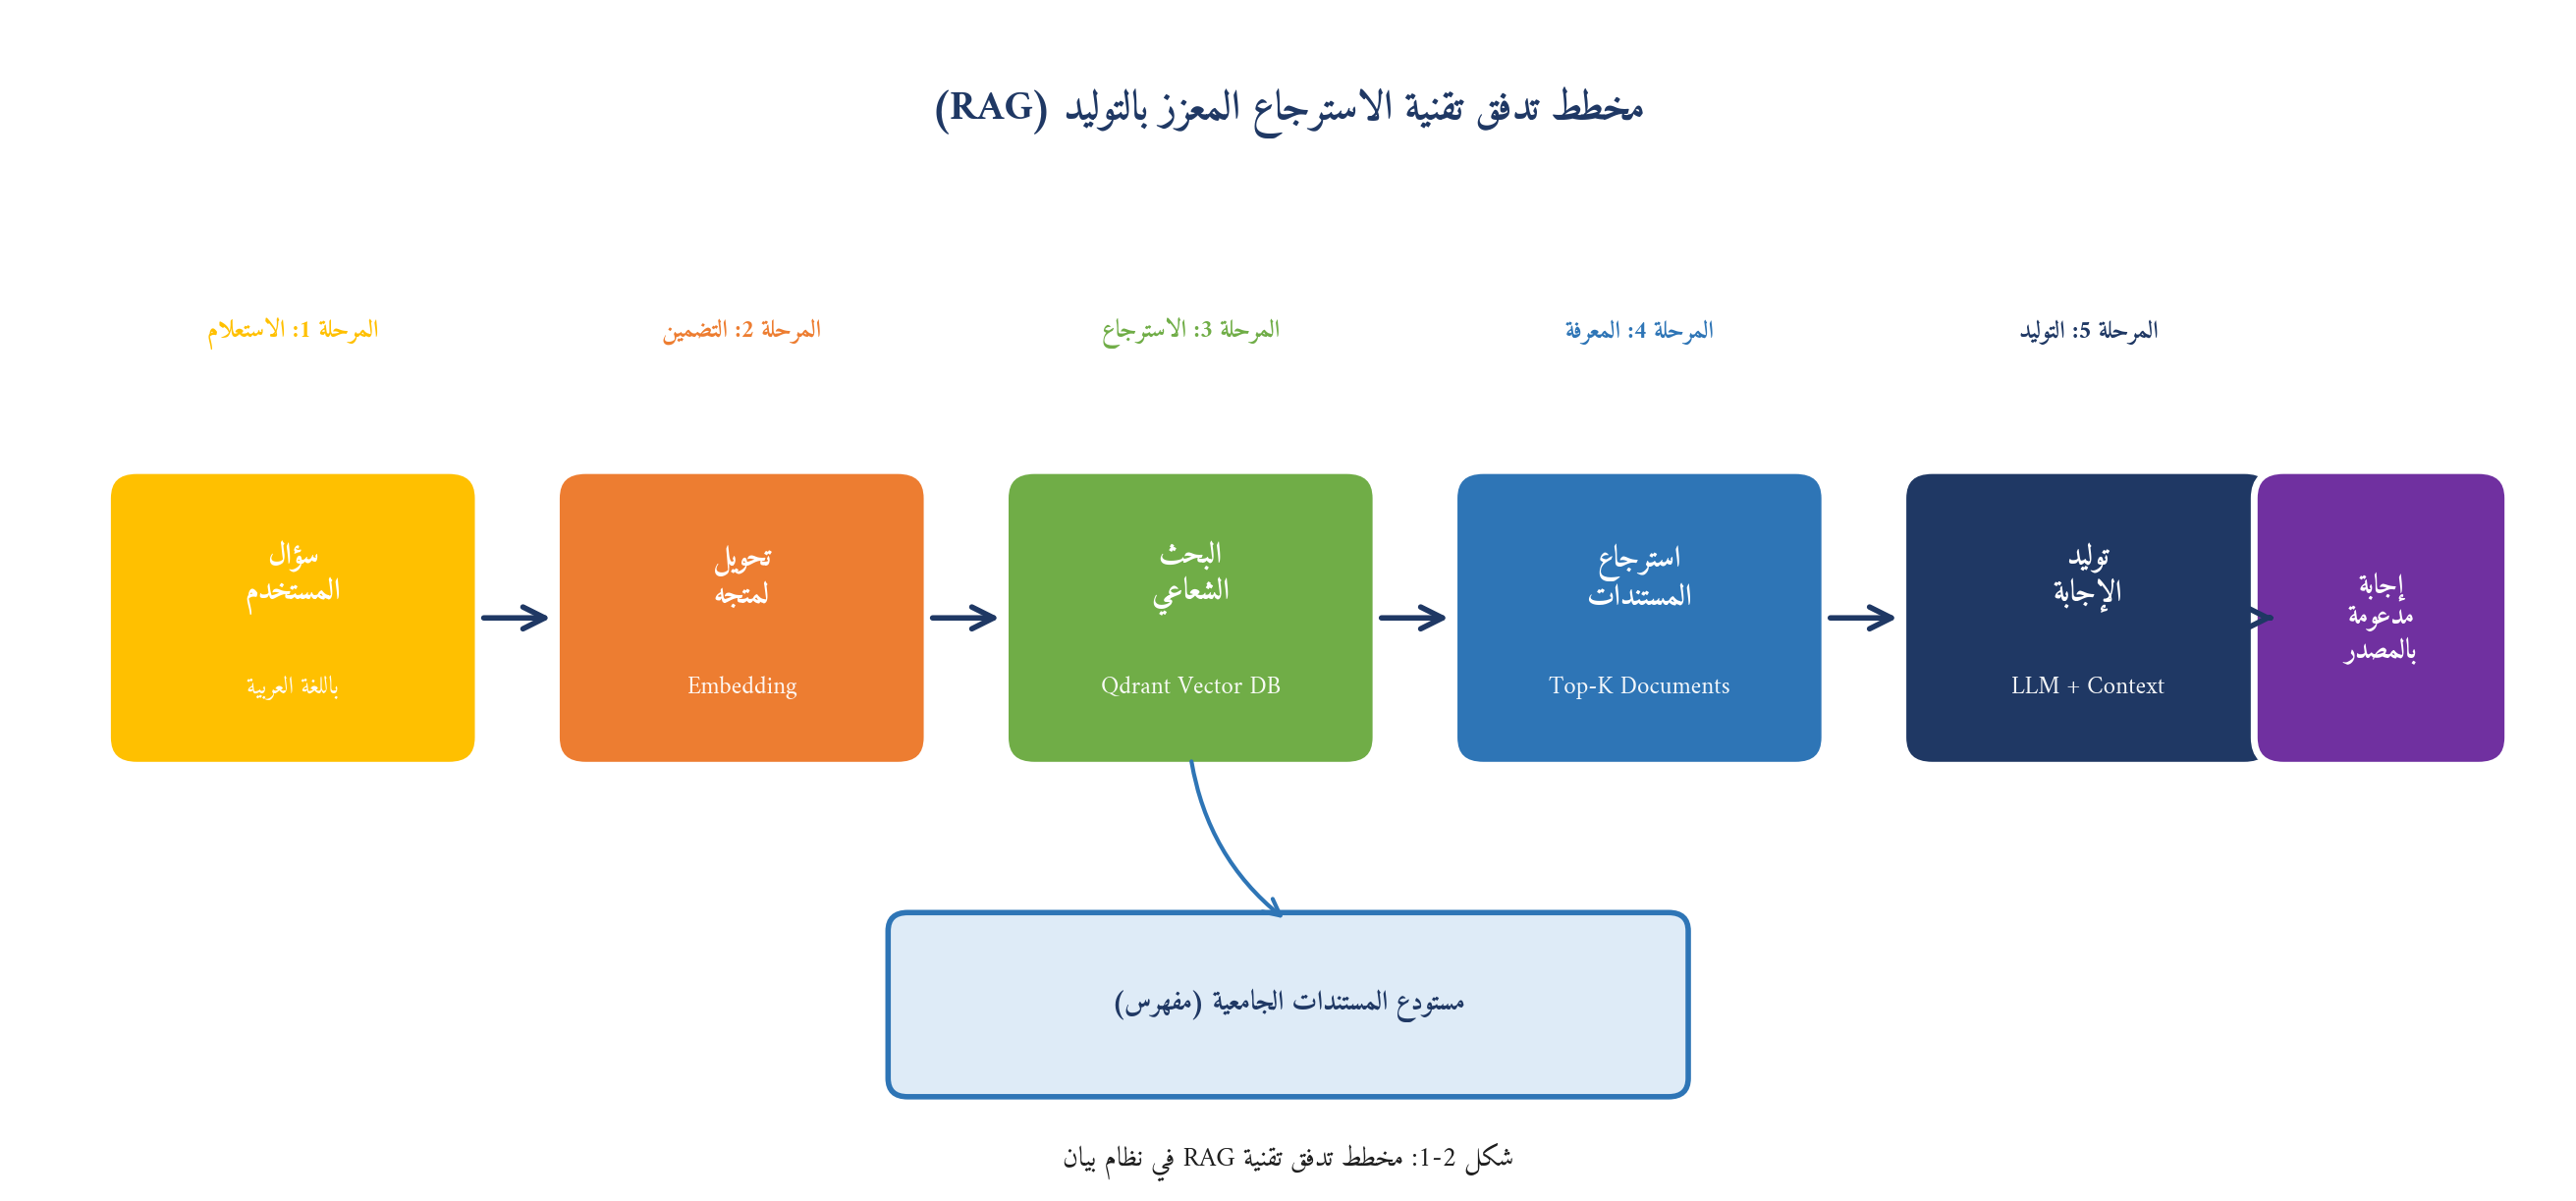
\includegraphics[width=0.85\textwidth]{rag-flow.png}
  \caption{مخطط تدفق تقنية \EN{RAG} في نظام بيان.}
  \label{fig:rag-flow}
\end{figure}

من أبرز الأطر الحالية لبناء أنظمة \EN{RAG}، يأتي \EN{LangChain}
\cite{langchain2023} في المقدمة كإطار العمل الأكثر انتشاراً، ويقدم مكونات
قابلة للتخصيص للبحث والتوليد. ويأتي \EN{LlamaIndex} \cite{llamaindex2023}
كإطار متخصص في \EN{RAG}، يقدم أدوات متقدمة لفهرسة المستندات وإدارة السياق.
كما تقدم \EN{Microsoft} خدمة \EN{Azure AI Search} المتكاملة مع \EN{RAG}،
وتقدم \EN{Google} خدمة \EN{Vertex AI Search}.

يعتمد أداء \EN{RAG} بشكل جوهري على جودة نظام الاسترجاع، والذي يتطلب قاعدة
بيانات شعاعية (\EN{Vector Database}) متخصصة. وقد ظهرت عدة حلول مفتوحة المصدر
وتجارية في السنوات الأخيرة، أبرزها \EN{Qdrant} \cite{qdrant2024} الذي اعتمد
عليه مشروع بيان، و \EN{Pinecone} التجاري، و \EN{Milvus}، إضافة إلى امتداد
\EN{pgvector} لـ \EN{PostgreSQL}.

\subsection{الأنظمة متعددة الوكلاء (\EN{Multi-Agent Systems})}
\label{subsec:multi-agent}

تُعرَّف الأنظمة متعددة الوكلاء في سياق الذكاء الاصطناعي الحديث بأنها أنظمة
تُكلف فيها عدة وكلاء مستقلين بإجراء مهام متخصصة، مع وجود آلية تنسيق تضمن
تكامل مخرجاتهم. وقد ظهر هذا المفهوم بقوة منذ عام 2023 مع تطور قدرات النماذج
اللغوية، حيث أصبح كل وكيل عبارة عن \EN{LLM} مُوجَّه بمهمة وشخصية محددة.

يُعدّ إطار \EN{LangGraph} \cite{langgraph2024} من \EN{LangChain} الأبرز في
هذا المجال، ويستخدم نظرية المخططات لتمثيل تدفق العمل بين الوكلاء كعقد
(\EN{Nodes}) وحواف (\EN{Edges}). يتميز بتحكم دقيق في التدفق ودعم الحلقات
التكرارية والتفرعات المشروطة، وهو ما اعتمد عليه مشروع بيان. ويأتي إطار
\EN{AutoGen} \cite{wu2023autogen} من \EN{Microsoft Research} كخيار مرن قائم
على المحادثات بين الوكلاء، لكنه يعاني من زيادة في استهلاك الـ \EN{Tokens}.

إطار \EN{CrewAI} \cite{crewai2024} هو إطار حديث أطلق عام 2024، يركز على
محاكاة فرق العمل البشرية بأدوار محددة، ويتميز بسهولة الاستخدام. أما إطار
\EN{MetaGPT} \cite{hong2023metagpt} فيقدم نهجاً مختلفاً، حيث يحاكي فريق تطوير
برمجيات تقليدي (\EN{Product Manager, Architect, Engineer}) لإنتاج شفرات
برمجية متكاملة، وقد حقق تفوقاً ملحوظاً في إنتاج الكود الصحيح.

تُظهر هذه المراجعة أن \EN{LangGraph} هو الإطار الأنسب لمشروع بيان، نظراً
لكونه يدعم بناء أنظمة معقدة ذات وكلاء متخصصين، مع إمكانية تتبع مسار التنفيذ
(\EN{Agent Trace}) المطلوبة للشفافية في البيئة الجامعية.

\begin{figure}[!htbp]
  \centering
  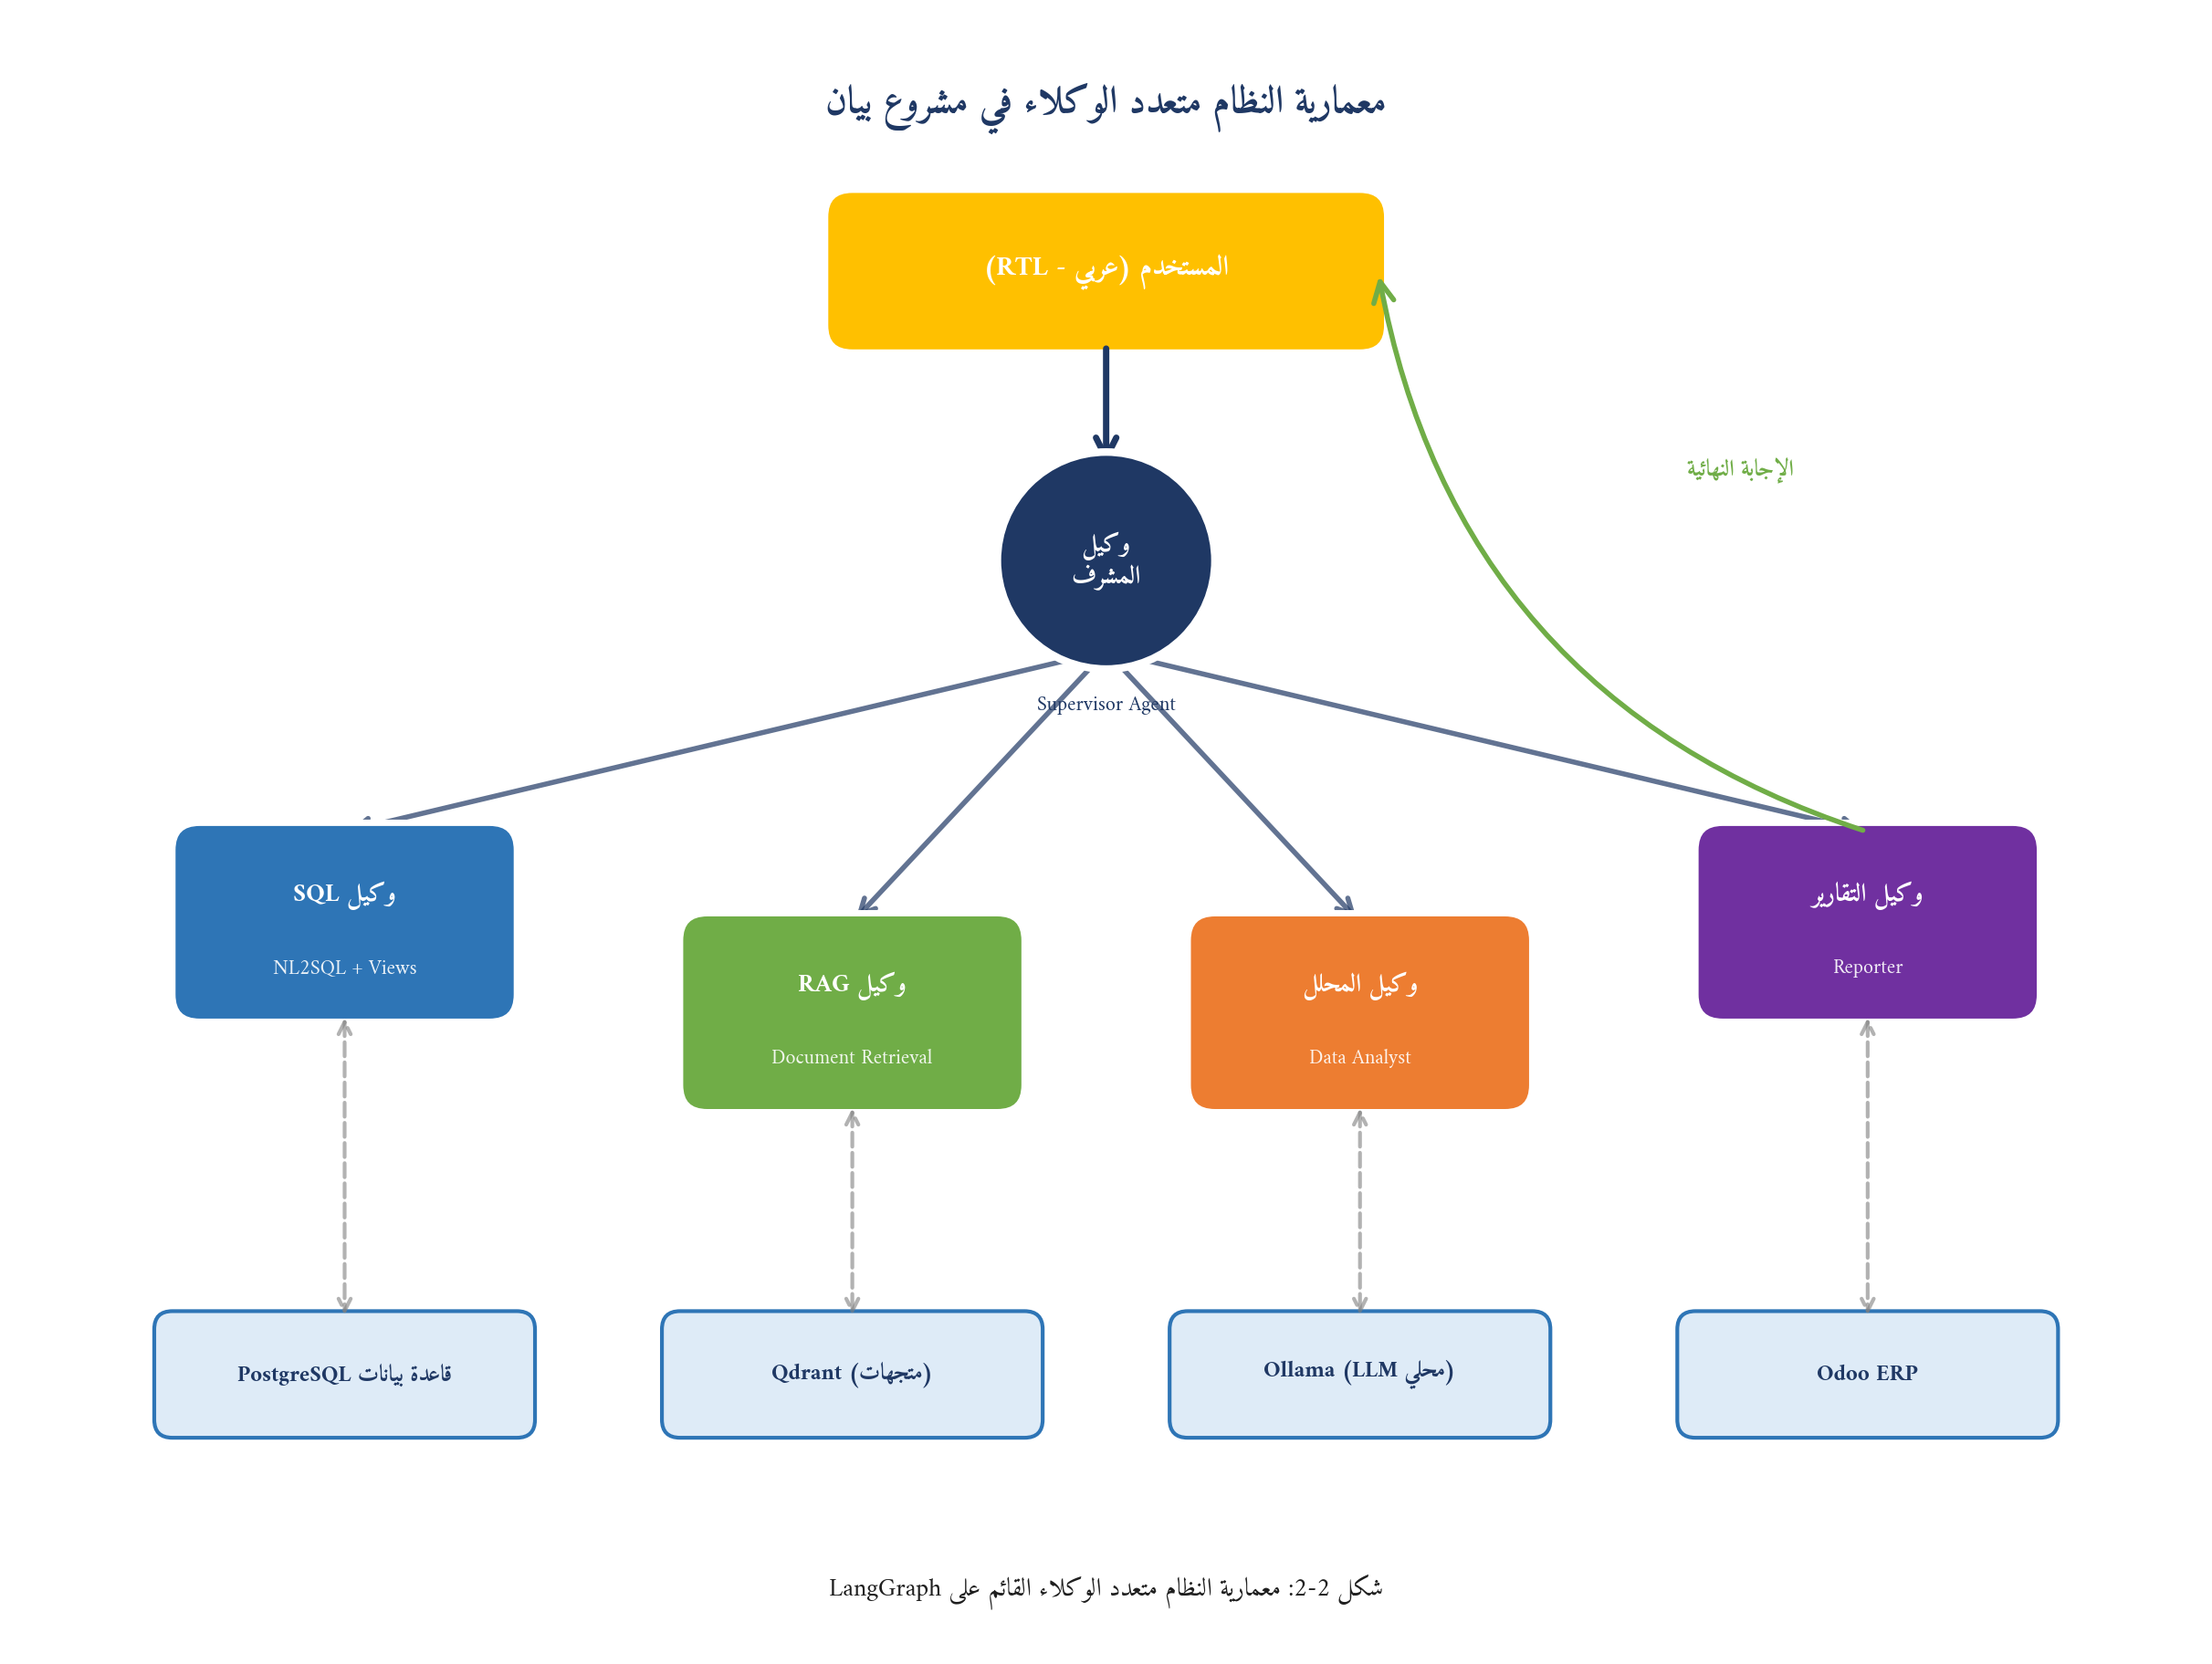
\includegraphics[width=0.7\textwidth]{multi-agent-arch.png}
  \caption{معمارية النظام متعدد الوكلاء القائم على \EN{LangGraph}.}
  \label{fig:multi-agent}
\end{figure}

\subsection{تحديات معالجة اللغة العربية (\EN{Arabic NLP})}
\label{subsec:arabic-nlp}

تواجه معالجة اللغة العربية طبيعياً تحديات جوهرية تختلف عن نظيراتها في اللغة
الإنجليزية، وتعود هذه التحديات إلى عوامل لغوية وتقنية \cite{elhaij2023arabic}.
فمن الناحية اللغوية، تتميز العربية بالصرف الغني حيث يمكن اشتقاق عشرات الكلمات
من جذر واحد ثلاثي، مما يزيد من حجم المفردات وصعوبة التطابق. كما تتميز بتركيب
الجملة المرن الذي يصعّب التحليل النحوي الآلي، وظاهرة الإعراب التي تُغير الحركة
النهائية للكلمات.

أما من الناحية التقنية، فتعاني العربية من فجوة الموارد الحادة؛ إذ تشير
الإحصائيات إلى أن نسبة المحتوى العربي على الإنترنت لا تتجاوز 1.2\% من
الإجمالي، في حين أن المتحدثين بالعربية يشكلون نحو 5\% من سكان العالم
\cite{elhaij2023arabic}. وتعتمد معظم التطبيقات التجارية على نماذج إنجليزية
تُظهر أداءً ضعيفاً على العربية، وتشمل النماذج المدعومة للعربية: \EN{Jais}
النموذج الإماراتي المتخصص في العربية، و \EN{AraBERT} النموذج المبني على
\EN{BERT} والمتخصص في النصوص العربية، و \EN{Qwen 2.5} من \EN{Alibaba} الذي
يدعم العربية جزئياً ويتميز بكفاءة عالية في المهام البرمجية.

تتفاقم هذه التحديات في السياق اليمني تحديداً، حيث تُستخدم لهجة محلية تختلف عن
الفصحى والعاميات الخليجية والمصرية، وغير مدعومة بأي موارد برمجية معروفة.
ولهذا السبب، يعتمد مشروع بيان استراتيجية لغوية مرنة تقبل الفصحى والعامية، مع
الاستفادة من قدرة النماذج اللغوية الحديثة على التعميم بدلاً من تدريب نموذج
متخصص.

%------------------------------------------------------------------------------
\section{الأنظمة والدراسات السابقة}
\label{sec:related-work}

تم تصنيف الأنظمة والدراسات السابقة المراجعة في خمس فئات رئيسية، وفقاً لمجال
التخصص وارتباطها بمشروع بيان. وقد رُوعي في الاختيار التركيز على الأنظمة
الحديثة (2021-2025) والتجارية المتاحة فعلياً.

\subsection{الأنظمة في مجال تحويل اللغة الطبيعية إلى \EN{SQL}}
يُعدّ معيار \EN{Spider} الذي أُطلق عام 2018 المرجع القياسي لتقييم أنظمة
\EN{NL2SQL}، حيث يضم 10,181 سؤالاً عبر 200 قاعدة بيانات. وفي عام 2023،
أُطلق معيار \EN{BIRD} الأكثر تحدياً لتركيزه على قواعد البيانات الواقعية مع
قيم شاذة وأخطاء. حققت أفضل الأنظمة 40\% فقط على \EN{BIRD} مقابل 60\% على
\EN{Spider}، مما يُبرز فجوة الأداء في البيئات الواقعية \cite{yu2023spider}.

من أبرز الأنظمة الحالية في هذا المجال، يُبرز نظام \EN{Vanna.ai}
\cite{vanna2024} كأحد أكثر الأطر مفتوحة المصدر انتشاراً. يعتمد \EN{Vanna} على
دمج \EN{RAG} مع \EN{NL2SQL}، ويتدرب على قاعدة بيانات كل عميل لرفع الدقة.
أما نظام \EN{Snowflake Arctic-Text2SQL-R1} \cite{snowflake2025arctic} فهو
نموذج متخصص أطلق أوائل 2025، يستخدم تقنية التعلم المعزز في التدريب ويحقق
71.83\% على معيار \EN{BIRD}.

تجدر الإشارة إلى أن جميع هذه الأنظمة مصممة للبيئة الإنجليزية، ولا تقدم دعماً
كافياً للغة العربية. كما أنها تعمل كأنظمة أحادية (\EN{Single-Agent})، ولا
تستفيد من البنية متعددة الوكلاء في المهام المعقدة.

\subsection{الأنظمة في مجال الاسترجاع المعزز بالتوليد (\EN{RAG})}
منذ تقديم مفهوم \EN{RAG} بشكلها الحديث عام 2020 \cite{lewis2020rag}، شهدت
هذه التقنية تطوراً متسارعاً وأصبحت المعيار الذهبي لتطبيقات \EN{LLM} المؤسسية.
أظهرت الدراسات أن \EN{RAG} يقلل الهلوسة بنسبة تصل إلى 50\% مقارنة بالنماذج
اللغوية التقليدية، مما جعله خياراً مفضلاً للتطبيقات التي تتطلب دقة عالية.

من أبرز الأطر الحالية لبناء أنظمة \EN{RAG}، يأتي \EN{LangChain}
\cite{langchain2023} في المقدمة كإطار العمل الأكثر انتشاراً، ويقدم مكونات
قابلة للتخصيص للبحث والتوليد. ويأتي \EN{LlamaIndex} \cite{llamaindex2023}
كإطار متخصص في \EN{RAG}، يقدم أدوات متقدمة لفهرسة المستندات وإدارة السياق.
كما تقدم \EN{Microsoft} خدمة \EN{Azure AI Search} المتكاملة مع \EN{RAG}،
وتقدم \EN{Google} خدمة \EN{Vertex AI Search}.

على صعيد قواعد البيانات الشعاعية، يبرز \EN{Qdrant} \cite{qdrant2024} كحل
مفتوح المصدر يتميز بأداء عالٍ ودعم فلترة المتجهات بالبيانات الوصفية، وهو ما
اعتمد عليه مشروع بيان. كما تقدم \EN{Pinecone} حلاً تجارياً سحابياً، ويقدم
\EN{Milvus} حلاً مفتوحاً موزعاً. وفي سياق قواعد البيانات العلائقية، يقدم
امتداد \EN{pgvector} لـ \EN{PostgreSQL} إمكانية البحث الشعاعي دون الحاجة
لقاعدة بيانات منفصلة.

\subsection{الأنظمة في مجال الأنظمة متعددة الوكلاء}
رغم التطور المتسارع الذي شهدته الأنظمة متعددة الوكلاء منذ عام 2023 (انظر
المراجعة التفصيلية في القسم~\ref{subsec:multi-agent})، فإن التطبيقات المؤسسية
الجاهزة التي تعتمد هذه البنية لا تزال محدودة. تتركز الأطر المتاحة
(\EN{LangGraph}، \EN{AutoGen}، \EN{CrewAI}، \EN{MetaGPT}) على المستوى
التقني لبناء الوكلاء، دون تقديم حلول جاهزة للمؤسسات. هذا يعني أن أي مؤسسة
ترغب في اعتماد البنية متعددة الوكلاء مطالبة ببناء نظامها من الصفر، وهو ما يفسر
ندرة الأنظمة المؤسسية المبنية على هذه التقنية، ويبرر أهمية مشروع بيان الذي
يقدم تطبيقاً ميدانياً متكاملاً للبنية متعددة الوكلاء في بيئة جامعية.

\subsection{المساعدات الذكية في التعليم العالي}
رغم الانتشار الواسع للمساعدات الذكية في مجال خدمة العملاء، تبقى التطبيقات
المتخصصة في التعليم العالي محدودة. أطلقت \EN{OpenAI} عام 2024 خدمة
\EN{ChatGPT Edu} المخصصة للجامعات، التي تتيح بناء مساعدات مخصصة لكل مؤسسة.
ومع ذلك، تظل هذه الخدمة عامة ولا تدمج \EN{NL2SQL} للاستعلام عن قواعد البيانات
الجامعية.

تقدم \EN{Microsoft} خدمة \EN{Copilot for Education} مع تكاملات محدودة مع
أنظمة إدارة التعلم (\EN{LMS}) مثل \EN{Canvas} و \EN{Blackboard}، لكنها لا
تدعم العربية بشكل كامل. كما تقدم \EN{Anthropic} خدمة \EN{Claude for
Education} التي تركز على المساعدة الأكاديمية للطلاب.

على الصعيد العربي، أطلقت العديد من الجامعات مساعدات ذكية بسيطة للأسئلة
الشائعة، لكنها تعتمد على قواعد معرفة محدودة ولا تستفيد من تقنيات \EN{RAG}
أو \EN{NL2SQL}. وأكدت دراسة \EN{Al-Khalifa} وآخرين \cite{alkhalifa2023} أن
معظم الجامعات العربية تستخدم \EN{chatbots} بسيطة دون الاستفادة من التقنيات
المتقدمة.

تُبرز هذه المراجعة أن الميدان يفتقر إلى نظام متكامل يجمع بين \EN{NL2SQL} و
\EN{RAG} والأنظمة متعددة الوكلاء في بيئة جامعية عربية، وهو ما يسعى مشروع
بيان لسده.

\subsection{الدراسات العربية}
على الصعيد العربي، تظل الدراسات في مجال المساعدات الذكية المؤسسية محدودة
وتتسم بالتشتت بين أربع اتجاهات رئيسية لا تلتقي عادةً في بحث واحد: معالجة
اللغة العربية، استرجاع المعلومات العربية، \EN{NL2SQL} للعربية، وتطبيقات
الذكاء الاصطناعي في التعليم.

دراسة \EN{Magdy} وآخرين \cite{magdy2024arabicir} استعرضت واقع البحث في
استرجاع المعلومات العربية، وأكدت أن الأنظمة التجارية تعاني من ضعف 30-40\% في
الدقة على العربية مقارنة بالإنجليزية. كما أكدت دراسة \EN{El-Haj}
\cite{elhaij2023arabic} المرجعية في معالجة اللغة العربية طبيعياً، أن المشاريع
العربية تواجه ثلاث تحديات رئيسية: ندرة \EN{corpora} عربية عالية الجودة، عدم
وجود معايير قياسية موحدة، وضعف التمويل البحثي.

أما في مجال \EN{NL2SQL} العربية تحديداً، فالدراسات شبه منعدمة. أغلب الأبحاث
العربية في قواعد البيانات تركز على واجهات التعبير النمطي أو الترجمة الآلية
للاستعلامات، دون الاستفادة من النماذج اللغوية الكبيرة. وقد رصدت دراسة
\EN{Al-Khalifa} \cite{alkhalifa2023} غياب أي نظام \EN{NL2SQL} عربي منشور حتى
عام 2023، مما يجعل مشروع بيان من الرواد في هذا المجال.

في مجال المساعدات الذكية التعليمية العربية، أطلقت جامعة الملك سعود عام 2022
مساعداً ذكياً للأسئلة الأكاديمية اعتمد على قاعدة معرفة ثابتة دون \EN{RAG}،
كما طوّرت جامعة الملك عبدالعزيز نظاماً مشابهاً لإرشاد الطلاب. لكن هذه
المحاولات تظل بسيطة ولا تدمج تقنيات الاسترجاع المعزز بالتوليد، ولا تدعم
الاستعلام عن قواعد البيانات الجامعية.

في البيئة اليمنية تحديداً، تكاد تنعدم الدراسات المنشورة في مجال الذكاء
الاصطناعي المؤسسي. وأكد تقرير الأمم المتحدة للتحول الرقمي
\cite{un2024egd} أن اليمن تحتل المرتبة 175 عالمياً في مؤشر تطور الحكومة
الإلكترونية. ويُعزى ذلك إلى عوامل متعددة، تشمل: محدودية البنية التحتية
الرقمية، وضعف الاستثمار في البحث والتطوير، وندرة الكوادر المتخصصة. هذا الواقع
يُبرز أهمية مشروع بيان كمساهمة بحثية وتطبيقية في سد هذه الفجوة، حيث يقدم
أول نظام \EN{NL2SQL}+\EN{RAG} عربي مفتوح المصدر مخصص للبيئة الجامعية
اليمنية، مع توثيق كامل لمنهجيته وتقييم أدائه.

%------------------------------------------------------------------------------
\section{مقارنة الأنظمة السابقة}
\label{sec:comparison}

يقدم هذا القسم تحليلاً مقارناً للأنظمة والدراسات السابقة المراجعة، مع التركيز
على ستة أبعاد رئيسية: التقنيات المستخدمة، اللغة المدعومة، البيئة التطبيقية،
دقة \EN{NL2SQL}، دقة \EN{RAG}، والبنية المعمارية. ويُلخص
الجدول~\ref{tab:comparison} أبرز الأنظمة ومقارنتها بمشروع بيان.

\begin{table}[!htbp]
  \centering
  \caption{مقارنة شاملة بين الأنظمة السابقة ومشروع بيان.}
  \label{tab:comparison}
  \small
  \renewcommand{\arraystretch}{1.4}
  \begin{tabularx}{\textwidth}{|>{\raggedright\arraybackslash}p{2.5cm}|>{\raggedright\arraybackslash}X|>{\raggedright\arraybackslash}p{1.8cm}|>{\raggedright\arraybackslash}p{1.8cm}|>{\raggedright\arraybackslash}p{1.8cm}|>{\raggedright\arraybackslash}p{1.6cm}|>{\raggedright\arraybackslash}p{1.8cm}|}
    \hline
    \textbf{النظام/الإطار} & \textbf{التقنيات المستخدمة} & \textbf{اللغة} & \textbf{البيئة التطبيقية} & \textbf{دقة \EN{NL2SQL}} & \textbf{دقة \EN{RAG}} & \textbf{البنية} \\
    \hline
    \EN{Vanna.ai} \cite{vanna2024} (2024) & \EN{NL2SQL + RAG} & إنجليزية & تجارية & 80\%+ & غير مذكورة & أحادية \\
    \hline
    \EN{Arctic-Text2SQL} \cite{snowflake2025arctic} (2025) & \EN{NL2SQL + RL} & إنجليزية & تجارية & 71.83\% (\EN{BIRD}) & --- & أحادية \\
    \hline
    \EN{LangChain} \cite{langchain2023} (2023) & \EN{RAG + LLM} & متعددة & عامة & --- & عالية & أحادية \\
    \hline
    \EN{LlamaIndex} \cite{llamaindex2023} (2023) & \EN{RAG + LLM} & متعددة & عامة & --- & عالية & أحادية \\
    \hline
    \EN{AutoGen} \cite{wu2023autogen} (2023) & \EN{Multi-Agent} & إنجليزية & عامة & --- & --- & متعددة \\
    \hline
    \EN{CrewAI} \cite{crewai2024} (2024) & \EN{Multi-Agent} & إنجليزية & عامة & --- & --- & متعددة \\
    \hline
    \EN{MetaGPT} \cite{hong2023metagpt} (2024) & \EN{Multi-Agent} & إنجليزية & تطوير برمجي & --- & --- & متعددة \\
    \hline
    \EN{ChatGPT Edu} (2024) & \EN{LLM + RAG} & متعددة & تعليم عالٍ & --- & جيدة & أحادية \\
    \hline
    \EN{Qdrant} \cite{qdrant2024} (2024) & \EN{Vector DB} & متعددة & عامة & --- & عالية & --- \\
    \hline
    \textbf{مشروع بيان (المقترح)} & \EN{NL2SQL + RAG + Multi-Agent} & عربية (فصحى وعامية) & جامعي (يمني) & $\geq$ 85\% (مستهدف) & $\geq$ 80\% (مستهدف) & متعددة (\EN{LangGraph}) \\
    \hline
  \end{tabularx}
\end{table}

تكشف المقارنة عن عدة ملاحظات جوهرية. أولاً، تركز معظم الأنظمة في \EN{NL2SQL}
على البيئة الإنجليزية، مع غياب شبه تام للأنظمة العربية المتخصصة. ثانياً،
تعتمد الأنظمة المتقدمة مثل \EN{Vanna.ai} على دمج \EN{NL2SQL} و \EN{RAG}،
لكنها لا تستخدم البنية متعددة الوكلاء، مما يُحدها في المهام المعقدة. ثالثاً،
تفتقر التطبيقات في التعليم العالي إلى التكامل بين الاستعلام عن البيانات
الديناميكية والبحث في المستندات الثابتة.

كما يُلاحظ أن مشروع بيان هو الوحيد الذي يجمع بين التقنيات الأربع
(\EN{NL2SQL}، \EN{RAG}، \EN{Multi-Agent}، \EN{Arabic NLP}) في إطار موحد، مع
تخصيصه للبيئة الجامعية اليمنية. هذا التكامل يمثل نقطة قوة، لكنه في الوقت ذاته
يفرض تحديات تصميمية معقدة، خاصة في تنسيق الوكلاء وضمان جودة الأداء عبر
المكونات المختلفة.

%------------------------------------------------------------------------------
\section{الفجوة البحثية}
\label{sec:gap}

يتميز مشروع «بيان» بكونه النظام الوحيد — في حدود ما اطلعت عليه الدراسة — الذي
يجمع بين التقنيات الأربع الأساسية (\EN{NL2SQL}، \EN{RAG}، \EN{Multi-Agent
Systems}، \EN{Arabic NLP}) في إطار موحد ومحلي الاستضافة، مع تخصيصه المباشر
للبيئة المؤسسية والتعليمية. ورغم أن هذا التكامل يمثل نقطة قوة واضحة، إلا أنه
يفرض في الوقت ذاته تحديات تصميمية وتنفيذية معقدة، خاصة في تنسيق عمل الوكلاء
البرمجيين وضمان جودة الأداء والاعتمادية عبر المكونات المختلفة.

بناءً على المراجعة الشاملة للأنظمة والدراسات السابقة والتحليل المقارن، يمكن
تحديد الفجوة البحثية والتطبيقية التي يسعى مشروع «بيان» لسدها في \textbf{خمسة
محاور رئيسية}:

\textbf{المحور الأول — الفجوة التقنية:} رغم وجود أنظمة \EN{NL2SQL} متقدمة
(\EN{Vanna.ai}، \EN{Arctic-Text2SQL}) وأنظمة \EN{RAG} فعالة
(\EN{LangChain}، \EN{LlamaIndex})، إلا أنه لا يوجد نظام يجمع بين التقنيتين في
إطار موحد مع بنية متعددة الوكلاء. تعمل هذه الأنظمة بشكل منفرد، مما يُفقدها
التكامل المطلوب في البيئات المؤسسية المعقدة. مشروع بيان يسد هذه الفجوة عبر
الدمج العضوي للتقنيات الأربع (\EN{NL2SQL}، \EN{RAG}، \EN{Multi-Agent}،
\EN{Vector DB}).

\textbf{المحور الثاني — الفجوة اللغوية:} أكدت دراسات \EN{El-Haj}
\cite{elhaij2023arabic} و \EN{Magdy} \cite{magdy2024arabicir} على الفجوة
الواضحة في دعم اللغة العربية في أنظمة الذكاء الاصطناعي. تعاني الأنظمة
التجارية من انخفاض الدقة 30-40\% على العربية مقارنة بالإنجليزية، كما أنها غير
مصممة لفهم اللهجات المحلية. مشروع بيان يعالج هذه الفجوة عبر دعم العربية
الفصحى والعامية في واجهة محادثة \EN{RTL}، مع الاستفادة من نماذج \EN{Qwen} و
\EN{Jais} التي تدعم العربية.

\textbf{المحور الثالث — الفجوة التطبيقية} (\EN{Applied Gap}): تفتقر الأنظمة
التطبيقية في المؤسسات والقطاع الأكاديمي إلى التكامل بين الاستعلام عن البيانات
الرقمية والمالية (\EN{NL2SQL}) والبحث في اللوائح والسياسات والمستندات
التنظيمية (\EN{RAG}). تركز الأنظمة الحالية (مثل \EN{ChatGPT Enterprise} أو
\EN{ChatGPT Edu}) على جانب واحد فقط، مما يحد من قدرتها على تلبية الاحتياجات
التشغيلية الكاملة للمستفيدين. يقدم نظام «بيان» حلاً موحداً يدمج الجانبين عبر
وكلاء متخصصين.

\textbf{المحور الرابع — الفجوة السياقية:} الأنظمة التجارية مثل \EN{Vanna.ai}
و \EN{ChatGPT Edu} مصممة لبيئات تجارية غربية، ولا تأخذ في الاعتبار خصوصية
البيئة الجامعية اليمنية (اللوائح المحلية، اللهجة، البنية التحتية المحدودة).
مشروع بيان مصمم خصيصاً لهذه البيئة، مع استخدام \EN{Odoo ERP} كبيئة محاكاة
واقعية تُحقن ببيانات تعادل 15 عاماً.

\textbf{المحور الخامس — فجوة الابتكار:} لا توجد دراسة سابقة قدمت طبقة
\EN{Views} ذكية كآلية لتبسيط مخطط قاعدة البيانات وتحسين دقة \EN{NL2SQL}.
هذا الابتكار يمثل مساهمة بحثية أصلية يمكن البناء عليها في دراسات مستقبلية،
وقد يفتح آفاقاً جديدة في مجال \EN{Database Abstraction Layer}.

يُلخص الجدول~\ref{tab:gap} الفجوة البحثية ومساهمة مشروع بيان في سدها عبر
المحاور الخمسة.

\begin{table}[!htbp]
  \centering
  \caption{ملخص الفجوة البحثية ومساهمة مشروع بيان في سدها.}
  \label{tab:gap}
  \renewcommand{\arraystretch}{1.5}
  \begin{tabularx}{\textwidth}{|>{\raggedright\arraybackslash}p{2.5cm}|>{\raggedright\arraybackslash}X|>{\raggedright\arraybackslash}X|}
    \hline
    \textbf{المحور} & \textbf{الفجوة المحددة} & \textbf{مساهمة مشروع بيان} \\
    \hline
    تقنية & غياب الدمج بين \EN{NL2SQL} و \EN{RAG} و \EN{Multi-Agent} & دمج التقنيات الأربع في إطار موحد \\
    \hline
    لغوية & ضعف دعم العربية واللهجات & دعم فصحى وعامية في واجهة \EN{RTL} \\
    \hline
    تطبيقية & فصل الاستعلام عن البيانات عن البحث في المستندات & نظام موحد يجمع الجانبين \\
    \hline
    سياقية & غياب حلول مخصصة للبيئة المؤسسية والمحلية & تخصيص كامل للبيئة المؤسسية مع بيئة محاكاة لأكثر من نوع من قواعد البيانات \\
    \hline
    ابتكارية & غياب طبقة تجريدية مبسطة فوق قواعد البيانات & ابتكار طبقة \EN{Views} ذكية \\
    \hline
  \end{tabularx}
\end{table}

%------------------------------------------------------------------------------
\section{الخلاصة}
\label{sec:summary}

استعرض هذا الفصل الإطار النظري الشامل الذي يستند إليه \textbf{«مشروع المساعد
الذكي المؤسسي (بيان)»}، بدءاً من المفاهيم الأساسية في النماذج اللغوية الكبيرة
(\EN{LLMs})، مروراً بالتقنيات المتخصصة في \EN{NL2SQL} و \EN{RAG} والأنظمة
متعددة الوكلاء (\EN{Multi-Agent Systems})، وصولاً إلى تحديات معالجة اللغة
العربية طبيعياً (\EN{Arabic NLP}). وقد كشف الاستعراض النظري أن المشروع يعتمد
على ركائز علمية متينة ومثبتة، مع الاستفادة من أحدث الأطر والأدوات المتاحة
(2021-2025) في كل مجال.

كما قدم الفصل مراجعة شاملة للأنظمة والدراسات السابقة ومقارنة مرجعية بينها.
وأظهرت المراجعة أن مجال \EN{NL2SQL} شهد تقدماً كبيراً في السنوات الثلاث
الأخيرة مع ظهور أطر مثل \EN{Vanna.ai} و \EN{Arctic-Text2SQL}. وفي مجال
\EN{RAG}، أثبتت الأطر المتقدمة مثل \EN{LangChain} و \EN{LlamaIndex} كفاءتها
العالية. وفي مجال الأنظمة متعددة الوكلاء، أظهر إطار \textbf{\EN{LangGraph}}
تفوقاً ملحوظاً في إدارة الحالات (\EN{State Management}) والتحكم في مسارات
التنفيذ.

كشف التحليل المقارن أن مشروع «بيان» يمثل خطوة متقدمة في الدمج الشامل للتقنيات
الأربع في بيئة عمل مؤسسية، حيث اتُخذت جامعة العلوم والتكنولوجيا كدراسة حالة
وتطبيق تجريبي. وخلص الفصل إلى تحديد خمسة محاور رئيسية للفجوة البحثية (تقنية،
لغوية، تطبيقية، سياقية، وابتكارية) يسعى المشروع لسدها، مما يُبرر القرارات
التصميمية والهندسية المتخذة، ويهيئ القارئ للفصل الثالث الذي يقدم تحليلاً
تفصيلياً للمتطلبات والمنهجية المتبعة في تطوير النظام.

%==============================================================================
% Chapter 3 — Methodology & System Analysis
%==============================================================================
\chapter{المنهجية وتحليل النظام}
\label{ch:analysis}
\markboth{الفصل الثالث: المنهجية وتحليل النظام}{الفصل الثالث: المنهجية وتحليل النظام}

%------------------------------------------------------------------------------
% 3.1 منهجية التطوير
%------------------------------------------------------------------------------
\section{منهجية التطوير}
\label{sec:methodology}

اعتمد فريق العمل منهجية التطوير الرشيقة \EN{Agile} \cite{schwaber2020scrum} في بناء نظام «بيان»، وذلك
لمواءمتها مع طبيعة المشروع الذي يجمع بين مكونات برمجية وتقنيات ذكاء اصطناعي
متقدمة، مثل توليد استعلامات قواعد البيانات من اللغة الطبيعية \EN{NL2SQL}،
والاسترجاع المعزز بالتوليد \EN{RAG}، ومعالجة اللغة العربية، وإدارة الأنظمة
متعددة الوكلاء المنسقة باستخدام إطار \EN{LangGraph}.

وتتطلب هذه التقنيات تكراراً مستمراً في تحسين النماذج اللغوية الكبيرة
\EN{LLMs}، والمطالبات \EN{Prompts}، وهيكلة المعرفة، فضلاً عن التحقق المتكرر
من دقة النتائج وزمن الاستجابة. لذلك، تقسم المنهجية الرشيقة نطاق العمل إلى
دورات تطوير قصيرة ومحددة زمنياً تسمى التكرارات أو الدورات \EN{Iterations / Sprints}.
وفي نهاية كل دورة، تُراجع المخرجات وتُقيّم قبل الانتقال إلى الدورة اللاحقة،
مما يتيح التكيف السريع مع التغيرات في المتطلبات أو مع نتائج تقييم النماذج
اللغوية دون التأثير الجوهري في الجدول الزمني العام للمشروع.

\subsection{دورة التطوير الرشيقة}
\label{subsec:agile-lifecycle}

تتكون كل دورة تطوير في مشروع «بيان» من ست مراحل متتابعة، مع إمكانية تكرارها
عند ظهور متطلبات جديدة أو الحاجة إلى تحسين أحد المكونات. وتضمن هذه المراحل
الانتقال المنظم من تحديد نطاق العمل إلى التقييم والتحسين، كما هو موضح في
الجدول \ref{tab:agile-phases}.

\begin{table}[H]
  \centering
  \caption{مراحل دورة التطوير الرشيقة المطبقة في مشروع «بيان».}
  \label{tab:agile-phases}
  \small
  \renewcommand{\arraystretch}{1.35}
  \begin{tabularx}{\textwidth}{>{\centering\arraybackslash}p{2.8cm}>{\raggedright\arraybackslash}X>{\raggedright\arraybackslash}p{4.1cm}}
    \toprule
    \textbf{المرحلة} & \textbf{أبرز الأنشطة} & \textbf{المخرج الرئيسي} \\
    \midrule
    \textbf{التخطيط}\\[-2pt]\EN{Planning}
    & تحديد أهداف الدورة الحالية، وإعداد قائمة مهام الدورة \EN{Sprint Backlog}،
      ومراجعة المتطلبات الوظيفية وغير الوظيفية المرتبطة بالمكون المستهدف.
    & وثيقة نطاق الدورة وقائمة المهام المحددة. \\
    \midrule
    \textbf{التصميم}\\[-2pt]\EN{Design}
    & نمذجة المعمارية الفنية للوكيل المستهدف، وتحديد هياكل البيانات والواجهات
      البرمجية \EN{APIs}، وإعداد التصميم الأولي لهندسة المطالبات \EN{Prompt Engineering}.
    & مخططات التدفق، وهياكل البيانات، ومخطط هندسة المطالبات. \\
    \midrule
    \textbf{التطوير}\\[-2pt]\EN{Development}
    & كتابة الشفرة البرمجية باستخدام \EN{Python} و\EN{FastAPI} و\EN{LangGraph}
      للواجهة الخلفية، أو \EN{Next.js} للواجهة الأمامية، وربط الوكلاء بمصادر
      البيانات \EN{PostgreSQL} و\EN{Qdrant}.
    & مكون برمجي جاهز يعمل بصورة مستقلة، مثل وكيل متخصص أو واجهة النظام. \\
    \midrule
    \textbf{الاختبار}\\[-2pt]\EN{Testing}
    & تنفيذ اختبارات الوحدة \EN{Unit Testing} واختبارات التكامل
      \EN{Integration Testing}، ومعايرة دقة الاستعلامات، والحد من الهلوسة،
      وقياس مؤشرات الأداء المعتمدة.
    & تقرير اختبارات موثق يوضح نسب الدقة وزمن الاستجابة. \\
    \midrule
    \textbf{الإطلاق والدمج}\\[-2pt]\EN{Deployment}
    & بناء المكونات البرمجية وحزمها داخل حاويات \EN{Docker Compose}، ودمجها
      في البيئة الموحدة، والتحقق من توافقها مع بقية الوكلاء.
    & نسخة محدثة من النظام، مدمجة ومجربة في بيئة التطوير. \\
    \midrule
    \textbf{المراجعة والتقييم}\\[-2pt]\EN{Review}
    & تقديم عرض توضيحي للمخرجات أمام مشرف المشروع، وتوثيق الدروس المستفادة،
      وتحديث الأولويات وقائمة مهام الدورة التالية.
    & قائمة تحسينات وتعديلات معتمدة للدورة المباشرة التالية. \\
    \bottomrule
  \end{tabularx}
\end{table}

\subsection{الدورات التنفيذية للمشروع}
\label{subsec:project-sprints}

لضمان التنفيذ المنهجي لمكونات نظام «بيان»، قُسّم نطاق المشروع إلى أربع دورات
تطوير تكرارية متتالية، بحيث تركز كل دورة على مكون رئيسي أو مجموعة مترابطة من
المكونات، وتنتهي بمخرج قابل للتقييم والدمج مع بقية النظام.

\begin{figure}[htbp]
  \centering
  \resizebox{0.91\textwidth}{!}{%==============================================================================
% Professional vertical roadmap for Bayan's four development sprints.
% Vector-only TikZ artwork; no external images or icon packages are required.
%==============================================================================

\begin{tikzpicture}[
  x=1cm,
  y=1cm,
  line cap=round,
  line join=round,
  connector/.style={->, >=stealth, line width=1.25pt, draw=kaudark!65},
  card title/.style={font=\Large\bfseries, align=center},
  card body/.style={font=\normalsize, text=kaudark, align=center},
  number/.style={font=\fontsize{19}{22}\selectfont\bfseries, text=white},
]

%------------------------------------------------------------------------------
% Shared card geometry
%------------------------------------------------------------------------------
\def\CardLeft{-7.35}
\def\CardRight{7.35}
\def\CardHalfHeight{1.23}
\def\IconX{-6.05}
\def\TextX{0.25}
\def\BadgeX{6.95}

%==============================================================================
% Sprint 1 — SQL Agent and Smart Views
%==============================================================================
\def\CardY{5.25}
\definecolor{sprintone}{HTML}{17639A}

% Soft shadow and card surface
\fill[black!10, rounded corners=8pt]
  (\CardLeft+0.10,\CardY-\CardHalfHeight-0.10)
  rectangle (\CardRight+0.10,\CardY+\CardHalfHeight-0.10);
\filldraw[fill=sprintone!4, draw=sprintone, line width=1.15pt, rounded corners=8pt]
  (\CardLeft,\CardY-\CardHalfHeight)
  rectangle (\CardRight,\CardY+\CardHalfHeight);

% Icon medallion
\fill[white] (\IconX,\CardY) circle (0.91);
\draw[sprintone!65, line width=1.15pt] (\IconX,\CardY) circle (0.91);
\draw[sprintone!18, line width=3.5pt] (\IconX,\CardY) circle (0.98);

% Database icon
\filldraw[fill=sprintone!82, draw=sprintone, line width=0.7pt]
  (\IconX-0.48,\CardY+0.36) arc[start angle=180,end angle=360,x radius=0.48,y radius=0.16]
  -- (\IconX+0.48,\CardY-0.29)
  arc[start angle=0,end angle=-180,x radius=0.48,y radius=0.16] -- cycle;
\draw[white!90, line width=0.65pt]
  (\IconX-0.48,\CardY+0.05) arc[start angle=180,end angle=360,x radius=0.48,y radius=0.16];
\draw[white!90, line width=0.65pt]
  (\IconX-0.48,\CardY-0.25) arc[start angle=180,end angle=360,x radius=0.48,y radius=0.16];
\filldraw[fill=white, draw=sprintone, line width=0.65pt, rounded corners=1.5pt]
  (\IconX+0.02,\CardY-0.52) rectangle (\IconX+0.63,\CardY-0.06);
\node[font=\scriptsize\bfseries, text=sprintone] at (\IconX+0.325,\CardY-0.29) {\EN{SQL}};

% Title, divider, and body
\node[card title, text=sprintone] at (\TextX,\CardY+0.52) {\RL{دورة التطوير الأولى}};
\draw[sprintone!70, line width=0.75pt] (-3.35,\CardY+0.15) -- (3.85,\CardY+0.15);
\fill[sprintone] (0.25,\CardY+0.15) circle (0.055);
\node[card body] at (\TextX,\CardY-0.32)
  {\RL{تطوير وكيل قواعد البيانات وطبقة الرؤى الذكية}\\[-1pt]
   {\small\color{sprintone}\EN{SQL Agent \& Smart Views}}};

% Number badge
\filldraw[fill=sprintone, draw=sprintone!75!black, line width=0.8pt]
  (\CardRight-0.08,\CardY+0.64) -- (\BadgeX-0.98,\CardY+0.64) --
  (\BadgeX-1.36,\CardY) -- (\BadgeX-0.98,\CardY-0.64) --
  (\CardRight-0.08,\CardY-0.64) -- cycle;
\node[number] at (\BadgeX-0.48,\CardY) {01};

%==============================================================================
% Sprint 2 — RAG Agent and document indexing
%==============================================================================
\def\CardY{1.75}
\definecolor{sprinttwo}{HTML}{2F7D32}

\fill[black!10, rounded corners=8pt]
  (\CardLeft+0.10,\CardY-\CardHalfHeight-0.10)
  rectangle (\CardRight+0.10,\CardY+\CardHalfHeight-0.10);
\filldraw[fill=sprinttwo!4, draw=sprinttwo, line width=1.15pt, rounded corners=8pt]
  (\CardLeft,\CardY-\CardHalfHeight)
  rectangle (\CardRight,\CardY+\CardHalfHeight);

\fill[white] (\IconX,\CardY) circle (0.91);
\draw[sprinttwo!65, line width=1.15pt] (\IconX,\CardY) circle (0.91);
\draw[sprinttwo!18, line width=3.5pt] (\IconX,\CardY) circle (0.98);

% Document and search icon
\filldraw[fill=sprinttwo!88, draw=sprinttwo, line width=0.7pt, rounded corners=1.5pt]
  (\IconX-0.46,\CardY-0.55) rectangle (\IconX+0.28,\CardY+0.54);
\fill[white] (\IconX+0.02,\CardY+0.54) -- (\IconX+0.28,\CardY+0.28) --
  (\IconX+0.02,\CardY+0.28) -- cycle;
\draw[white, line width=0.75pt]
  (\IconX-0.29,\CardY+0.08) -- (\IconX+0.08,\CardY+0.08)
  (\IconX-0.29,\CardY-0.12) -- (\IconX+0.03,\CardY-0.12)
  (\IconX-0.29,\CardY-0.32) -- (\IconX-0.03,\CardY-0.32);
\draw[sprinttwo, line width=1.1pt] (\IconX+0.34,\CardY-0.21) circle (0.27);
\draw[sprinttwo, line width=1.4pt] (\IconX+0.54,\CardY-0.41) -- (\IconX+0.75,\CardY-0.62);

\node[card title, text=sprinttwo] at (\TextX,\CardY+0.52) {\RL{دورة التطوير الثانية}};
\draw[sprinttwo!70, line width=0.75pt] (-3.35,\CardY+0.15) -- (3.85,\CardY+0.15);
\fill[sprinttwo] (0.25,\CardY+0.15) circle (0.055);
\node[card body] at (\TextX,\CardY-0.32)
  {\RL{تطوير وكيل البحث وفهرسة المستندات واللوائح}\\[-1pt]
   {\small\color{sprinttwo}\EN{RAG Agent \& Document Indexing}}};

\filldraw[fill=sprinttwo, draw=sprinttwo!75!black, line width=0.8pt]
  (\CardRight-0.08,\CardY+0.64) -- (\BadgeX-0.98,\CardY+0.64) --
  (\BadgeX-1.36,\CardY) -- (\BadgeX-0.98,\CardY-0.64) --
  (\CardRight-0.08,\CardY-0.64) -- cycle;
\node[number] at (\BadgeX-0.48,\CardY) {02};

%==============================================================================
% Sprint 3 — Multi-agent integration and Arabic UI
%==============================================================================
\def\CardY{-1.75}
\definecolor{sprintthree}{HTML}{633A98}

\fill[black!10, rounded corners=8pt]
  (\CardLeft+0.10,\CardY-\CardHalfHeight-0.10)
  rectangle (\CardRight+0.10,\CardY+\CardHalfHeight-0.10);
\filldraw[fill=sprintthree!4, draw=sprintthree, line width=1.15pt, rounded corners=8pt]
  (\CardLeft,\CardY-\CardHalfHeight)
  rectangle (\CardRight,\CardY+\CardHalfHeight);

\fill[white] (\IconX,\CardY) circle (0.91);
\draw[sprintthree!65, line width=1.15pt] (\IconX,\CardY) circle (0.91);
\draw[sprintthree!18, line width=3.5pt] (\IconX,\CardY) circle (0.98);

% Supervisor/network icon
\foreach \ang in {30,90,150,210,270,330} {
  \draw[sprintthree!75, line width=0.8pt]
    (\IconX,\CardY) -- ++(\ang:0.56);
  \filldraw[fill=white, draw=sprintthree, line width=0.9pt]
    (\IconX,\CardY) ++(\ang:0.62) circle (0.12);
}
\filldraw[fill=sprintthree, draw=sprintthree!80!black, line width=0.7pt]
  (\IconX,\CardY) circle (0.34);
\fill[white] (\IconX,\CardY+0.10) circle (0.09);
\fill[white] (\IconX-0.16,\CardY-0.16)
  .. controls (\IconX-0.10,\CardY-0.03) and (\IconX+0.10,\CardY-0.03) ..
  (\IconX+0.16,\CardY-0.16) -- cycle;

\node[card title, text=sprintthree] at (\TextX,\CardY+0.52) {\RL{دورة التطوير الثالثة}};
\draw[sprintthree!70, line width=0.75pt] (-3.35,\CardY+0.15) -- (3.85,\CardY+0.15);
\fill[sprintthree] (0.25,\CardY+0.15) circle (0.055);
\node[card body] at (\TextX,\CardY-0.32)
  {\RL{دمج الوكلاء وبناء الواجهة العربية التفاعلية}\\[-1pt]
   {\small\color{sprintthree}\EN{Supervisor Agent \& Arabic Web Interface}}};

\filldraw[fill=sprintthree, draw=sprintthree!75!black, line width=0.8pt]
  (\CardRight-0.08,\CardY+0.64) -- (\BadgeX-0.98,\CardY+0.64) --
  (\BadgeX-1.36,\CardY) -- (\BadgeX-0.98,\CardY-0.64) --
  (\CardRight-0.08,\CardY-0.64) -- cycle;
\node[number] at (\BadgeX-0.48,\CardY) {03};

%==============================================================================
% Sprint 4 — Testing, optimization, and deployment
%==============================================================================
\def\CardY{-5.25}
\definecolor{sprintfour}{HTML}{D66A00}

\fill[black!10, rounded corners=8pt]
  (\CardLeft+0.10,\CardY-\CardHalfHeight-0.10)
  rectangle (\CardRight+0.10,\CardY+\CardHalfHeight-0.10);
\filldraw[fill=sprintfour!4, draw=sprintfour, line width=1.15pt, rounded corners=8pt]
  (\CardLeft,\CardY-\CardHalfHeight)
  rectangle (\CardRight,\CardY+\CardHalfHeight);

\fill[white] (\IconX,\CardY) circle (0.91);
\draw[sprintfour!65, line width=1.15pt] (\IconX,\CardY) circle (0.91);
\draw[sprintfour!18, line width=3.5pt] (\IconX,\CardY) circle (0.98);

% Gear/check icon
\foreach \ang in {0,45,...,315} {
  \fill[sprintfour] (\IconX,\CardY) ++(\ang:0.48)
    ++(-0.11,-0.13) rectangle ++(0.22,0.26);
}
\filldraw[fill=sprintfour, draw=sprintfour!80!black, line width=0.7pt]
  (\IconX,\CardY) circle (0.49);
\fill[white] (\IconX,\CardY) circle (0.32);
\draw[sprintfour, line width=1.35pt]
  (\IconX-0.18,\CardY) -- (\IconX-0.04,\CardY-0.14) --
  (\IconX+0.23,\CardY+0.17);

\node[card title, text=sprintfour] at (\TextX,\CardY+0.52) {\RL{دورة التطوير الرابعة}};
\draw[sprintfour!70, line width=0.75pt] (-3.35,\CardY+0.15) -- (3.85,\CardY+0.15);
\fill[sprintfour] (0.25,\CardY+0.15) circle (0.055);
\node[card body] at (\TextX,\CardY-0.32)
  {\RL{الاختبار الشامل وضبط الأداء والتجهيز للنشر}\\[-1pt]
   {\small\color{sprintfour}\EN{Testing, Optimization \& Deployment}}};

\filldraw[fill=sprintfour, draw=sprintfour!75!black, line width=0.8pt]
  (\CardRight-0.08,\CardY+0.64) -- (\BadgeX-0.98,\CardY+0.64) --
  (\BadgeX-1.36,\CardY) -- (\BadgeX-0.98,\CardY-0.64) --
  (\CardRight-0.08,\CardY-0.64) -- cycle;
\node[number] at (\BadgeX-0.48,\CardY) {04};

%------------------------------------------------------------------------------
% Connectors — drawn last to remain crisp between cards
%------------------------------------------------------------------------------
\draw[connector] (0,4.00) -- (0,3.03);
\draw[connector] (0,0.50) -- (0,-0.47);
\draw[connector] (0,-3.00) -- (0,-3.97);

% Subtle decorative dot fields at the outer margins
\foreach \y/\c in {5.25/sprintone,1.75/sprinttwo,-1.75/sprintthree,-5.25/sprintfour} {
  \foreach \dx in {0,0.18,0.36} {
    \foreach \dy in {-0.18,0,0.18} {
      \fill[\c!48] (-7.82+\dx,\y+\dy) circle (0.025);
      \fill[\c!48] (7.82-\dx,\y+\dy) circle (0.025);
    }
  }
}

\end{tikzpicture}
}
  \caption{خارطة الدورات التطويرية الأربع المعتمدة في مشروع «بيان».}
  \label{fig:project-sprints}
\end{figure}

\subsubsection{الدورة الأولى: بناء وكيل استعلام قواعد البيانات}
\label{subsubsec:sprint-one}

\textbf{المستهدف:} إعداد المعمارية الأساسية للتعامل مع البيانات المهيكلة في
قاعدة بيانات \EN{PostgreSQL}، مع ضمان أمن الاستعلامات.

\textbf{الأنشطة:} تطوير طبقة الرؤى الذكية \EN{Smart Views} لعزل الجداول
المعقدة، وبناء محرك تحويل النص إلى استعلام \EN{NL2SQL Engine}، وإدراج آليات
العزل للقراءة فقط \EN{Read-Only Sandboxing} لمنع التعديل غير المصرح به، ثم
اختبار دقة التوليد على استعلامات مالية وإدارية وأكاديمية.

\textbf{المخرج:} وكيل \EN{SQL} مستقل يعمل عبر \EN{FastAPI} ويسترجع البيانات
بدقة من الجداول المحددة مع الالتزام بقيود الوصول الآمن.

\subsubsection{الدورة الثانية: بناء وكيل البحث في المستندات واللوائح}
\label{subsubsec:sprint-two}

\textbf{المستهدف:} معالجة البيانات غير المهيكلة، بما في ذلك اللوائح والسياسات
والمستندات التنظيمية الخاصة بالجامعة والمؤسسات ذات الصلة.

\textbf{الأنشطة:} إعداد قاعدة البيانات المتجهة \EN{Qdrant Vector DB}، وتطوير
معالج للنصوص العربية وتجزئتها \EN{Text Chunking}، وإنشاء المتجهات
\EN{Embeddings} باستخدام نماذج داعمة للغة العربية، وبناء آلية استرجاع معزز
بالمصادر ترفق اسم المستند ورقم الصفحة مع الإجابة متى توفرت البيانات.

\textbf{المخرج:} وكيل \EN{RAG} متكامل يجيب عن الأسئلة النصية بإجابات دقيقة
ومدعومة بمراجع واضحة.

\subsubsection{الدورة الثالثة: دمج الوكلاء وبناء الواجهة الأمامية}
\label{subsubsec:sprint-three}

\textbf{المستهدف:} تحقيق التكامل بين المكونات البرمجية وإتاحة واجهة مستخدم
عربية سلسة.

\textbf{الأنشطة:} بناء الوكيل المشرف \EN{Supervisor Agent} باستخدام إطار
\EN{LangGraph} لتوجيه الاستفسارات \EN{Intent Routing} إلى الوكيل المختص
(وكيل \EN{SQL} أو وكيل \EN{RAG} أو كليهما)، وإدارة ذاكرة السياق
\EN{Context Management}، ثم تطوير واجهة محادثة تفاعلية باللغة العربية
وبدعم الاتجاه من اليمين إلى اليسار \EN{RTL} باستخدام \EN{Next.js} و\EN{Tailwind CSS}.

\textbf{المخرج:} نظام موحد متعدد الوكلاء يعمل عبر واجهة ويب عربية حوارية
متكاملة.

\subsubsection{الدورة الرابعة: الاختبار الشامل وضبط الأداء والنشر}
\label{subsubsec:sprint-four}

\textbf{المستهدف:} التحقق من موثوقية النظام، وإدارة المخاطر التقنية، وتجهيز
البيئة التشغيلية للنشر والتقييم.

\textbf{الأنشطة:} تنفيذ اختبارات شاملة من البداية إلى النهاية
\EN{End-to-End Testing}، وتقييم زمن الاستجابة وجودة الإجابات، وضبط أداء
النموذج اللغوي المحلي \EN{Qwen 2.5 14B} عبر \EN{Ollama}، ثم حزم النظام
بالكامل باستخدام \EN{Docker} و\EN{Docker Compose}.

\textbf{المخرج:} بيئة تشغيل موحدة قابلة للنشر السريع، تحتوي على مكونات نظام
«بيان» في حاويات مستقلة وجاهزة للتسليم والتطبيق التجريبي.

\subsection{ملخص الدورات ومخرجاتها}
\label{subsec:sprints-summary}

يلخص الجدول \ref{tab:sprints-summary} العلاقة بين كل دورة تطوير والمكون
المستهدف والأدوات المستخدمة والمخرج المباشر المتحقق منها.

\begin{table}[H]
  \centering
  \caption{الملخص التنفيذي للدورات الأربع في منهجية تطوير نظام «بيان».}
  \label{tab:sprints-summary}
  \footnotesize
  \renewcommand{\arraystretch}{1.55}
  \begin{tabularx}{\textwidth}{>{\centering\arraybackslash}p{1.5cm}>{\raggedright\arraybackslash}p{3.2cm}>{\raggedright\arraybackslash}X>{\raggedright\arraybackslash}p{3.8cm}}
    \toprule
    \textbf{الدورة} & \textbf{المكون المستهدف} & \textbf{الأنشطة والأدوات الرئيسية} & \textbf{المخرج النهائي المباشر} \\
    \midrule
    \EN{Sprint 1} & وكيل \EN{SQL} وطبقة \EN{Smart Views}
    & \EN{PostgreSQL}، و\EN{FastAPI}، ومحرك \EN{NL2SQL}، وطبقة الرؤى الذكية.
    & وكيل \EN{SQL} آمن ومستقل لاسترجاع البيانات المهيكلة. \\
    \midrule
    \EN{Sprint 2} & وكيل \EN{RAG} والبحث في المستندات
    & قاعدة \EN{Qdrant} المتجهة، والمتجهات الدلالية العربية، وتجزئة المستندات.
    & وكيل \EN{RAG} يجيب استناداً إلى السياسات واللوائح مع توثيق المصدر. \\
    \midrule
    \EN{Sprint 3} & دمج الوكلاء والواجهة الأمامية
    & الوكيل المشرف \EN{LangGraph}، و\EN{Next.js}، و\EN{Tailwind CSS}.
    & نظام هجين موحد يعمل عبر واجهة ويب عربية حوارية. \\
    \midrule
    \EN{Sprint 4} & الاختبار والتحسين والنشر
    & \EN{Docker Compose}، و\EN{Ollama (Qwen 2.5 14B)}، واختبارات
      \EN{End-to-End}.
    & نسخة تشغيلية محزمة وجاهزة للتقييم والتطبيق التجريبي. \\
    \bottomrule
  \end{tabularx}
\end{table}

وبذلك تحقق المنهجية تدرجاً عملياً يبدأ ببناء الوكلاء المتخصصين، ثم دمجهم في
معمارية متعددة الوكلاء، وينتهي بالاختبار الشامل والتجهيز للنشر. كما تسمح
المخرجات المرحلية بتقييم كل مكون بصورة مستقلة قبل اعتماده ضمن النظام الموحد.

%------------------------------------------------------------------------------
\section{دراسة الجدوى}
\label{sec:feasibility}

% ← أضف المحتوى هنا

%------------------------------------------------------------------------------
\section{تحليل المتطلبات}
\label{sec:requirements}

% ← أضف المحتوى هنا

\subsection{المتطلبات الوظيفية}
\label{subsec:functional-reqs}

% ← أضف المحتوى هنا

\subsection{المتطلبات غير الوظيفية}
\label{subsec:nonfunctional-reqs}

% ← أضف المحتوى هنا

%------------------------------------------------------------------------------
% 3.4 حالات الاستخدام
%------------------------------------------------------------------------------
\section{حالات الاستخدام}
\label{sec:use-cases}

توضح حالات الاستخدام كيفية تفاعل مستخدمي نظام «بيان» مع وظائفه الرئيسية، كما تحدد الحدود بين الفاعلين البشريين والمكونات الآلية التي تنفذ المعالجة الداخلية. ويعتمد هذا القسم على ثماني حالات استخدام تغطي الاستعلام عن البيانات، والبحث في المستندات، وإعداد التقارير، وإدارة المستخدمين ومصادر البيانات، والتدقيق، والتهيئة الأولية للنظام.

\subsection{نموذج الفاعلين}
\label{subsec:actor-model}

يضم النظام ثمانية فاعلين رئيسيين ينقسمون إلى فئتين: فاعلون خارجيون بشريون وفاعلون داخليون آليون. وقد صُمم هذا الفصل بحيث يتعامل المستخدم البشري مع نقطة دخول موحدة، بينما تتولى الوكلاء المتخصصون تحليل الطلب وتنفيذه وفق صلاحيات الوصول المحددة.

\begin{figure}[htbp]
  \centering
  % Actor classification — v3 (2026-09): two-level actor taxonomy.
% Level 1 = actor KIND (pattern): external human actor (top band,
% 4 types) vs internal AI-agent actor (bottom band, 5 types —
% Reporter Agent added for full consistency with ch1/ch2/arch).
% Every Arabic label is wrapped in \textarabic{} inside bidi's LTR
% environment (same proven fix as the Gantt charts) so word order
% renders correctly. Card order runs right-to-left to match Arabic
% reading; numbered badges (1-9) match the actors table in 3.4.1.
\newsavebox{\ActorsBox}%
\begin{lrbox}{\ActorsBox}%
\begin{LTR}%
\begin{tikzpicture}[
  font=\small,
  stickman/.pic={
    \draw[line width=1.1pt, #1] (0,0.4) circle (0.2);
    \draw[line width=1.1pt, #1] (0,0.2) -- (0,-0.3);
    \draw[line width=1.1pt, #1] (-0.3,0.06) -- (0,-0.06) -- (0.3,0.06);
    \draw[line width=1.1pt, #1] (0,-0.3) -- (-0.22,-0.75);
    \draw[line width=1.1pt, #1] (0,-0.3) -- (0.22,-0.75);
  },
  robot/.pic={
    \draw[line width=1pt, #1] (0,0.44) -- (0,0.58);
    \fill[#1] (0,0.65) circle (0.05);
    \draw[line width=1pt, #1, rounded corners=2.5pt] (-0.24,0.14) rectangle (0.24,0.44);
    \fill[#1] (-0.11,0.29) circle (0.045);
    \fill[#1] (0.11,0.29) circle (0.045);
    \draw[line width=1pt, #1, rounded corners=3pt] (-0.3,-0.44) rectangle (0.3,0.08);
    \draw[line width=1pt, #1] (0,-0.18) circle (0.1);
    \fill[#1] (0,-0.18) circle (0.035);
  },
  actorcard/.style={
    rounded corners=6pt, draw=#1!75, fill=white, line width=0.9pt,
    minimum width=3.7cm, minimum height=3.05cm
  },
  actornum/.style={
    circle, fill=#1, text=white, font=\bfseries\scriptsize,
    inner sep=0pt, minimum size=0.42cm
  },
  actorname/.style={
    align=center, font=\bfseries\scriptsize, text=kaudark,
    inner sep=0pt
  },
  actoreng/.style={
    align=center, font=\tiny, text=kaudark!70, inner sep=0pt
  },
  actordesc/.style={
    align=center, font=\tiny, text=kaudark!85, inner sep=0pt,
    text width=3.25cm
  },
  actordescn/.style={
    align=center, font=\tiny, text=kaudark!85, inner sep=0pt,
    text width=2.5cm
  },
  bandpill/.style={
    rounded corners=4pt, fill=#1, text=white, inner sep=5pt,
    font=\bfseries\scriptsize
  }
]

  % ================= KIND 1: external human actor (4 types) =================
  \fill[kauprimary!6, rounded corners=10pt] (0.15,0.62) rectangle (15.85,-3.95);
  \node[bandpill=kauprimary] at (8.0,0.55)
    {\textarabic{النمط الأول: الفاعل البشري الخارجي — أربعة أنواع}};

  % Type 1 (rightmost): Enterprise Employee
  \draw[actorcard=kauprimary] (12.1,-0.55) rectangle (15.8,-3.6);
  \pic at (13.95,-1.35) {stickman={kaudark}};
  \node[actornum=kauprimary] at (15.45,-0.85) {\EN{1}};
  \node[actorname] at (13.95,-2.28) {\textarabic{موظف المؤسسة}};
  \node[actoreng]  at (13.95,-2.62) {\EN{Enterprise Employee}};
  \node[actordesc] at (13.95,-3.05) {\textarabic{إدخال الاستعلامات الأساسية والبحث في اللوائح والسياسات}};

  % Type 2: Enterprise Manager
  \draw[actorcard=kauprimary] (8.15,-0.55) rectangle (11.85,-3.6);
  \pic at (10.0,-1.35) {stickman={kaudark}};
  \node[actornum=kauprimary] at (11.5,-0.85) {\EN{2}};
  \node[actorname] at (10.0,-2.28) {\textarabic{مدير المؤسسة}};
  \node[actoreng]  at (10.0,-2.62) {\EN{Enterprise Manager}};
  \node[actordesc] at (10.0,-3.05) {\textarabic{الاطلاع على التقارير المتقدمة ومتابعة المؤشرات التشغيلية}};

  % Type 3: System Administrator
  \draw[actorcard=kauprimary] (4.2,-0.55) rectangle (7.9,-3.6);
  \pic at (6.05,-1.35) {stickman={kaudark}};
  \node[actornum=kauprimary] at (7.55,-0.85) {\EN{3}};
  \node[actorname] at (6.05,-2.28) {\textarabic{مسؤول النظام}};
  \node[actoreng]  at (6.05,-2.62) {\EN{System Administrator}};
  \node[actordesc] at (6.05,-3.05) {\textarabic{إدارة المستخدمين والأدوار وضبط الصلاحيات وسجلات التدقيق}};

  % Type 4: Onboarding Operator
  \draw[actorcard=kauprimary] (0.25,-0.55) rectangle (3.95,-3.6);
  \pic at (2.1,-1.35) {stickman={kaudark}};
  \node[actornum=kauprimary] at (3.6,-0.85) {\EN{4}};
  \node[actorname] at (2.1,-2.28) {\textarabic{مشغل التهيئة}};
  \node[actoreng]  at (2.1,-2.62) {\EN{Onboarding Operator}};
  \node[actordesc] at (2.1,-3.05) {\textarabic{ربط النظام بالمؤسسات الجديدة وتهيئة البيانات لأول مرة}};

  % ============ KIND 2: internal AI-agent actor (5 types) ============
  \fill[kausecondary!6, rounded corners=10pt] (0.15,-4.35) rectangle (15.85,-8.92);
  \node[bandpill=kausecondary] at (8.0,-4.42)
    {\textarabic{النمط الثاني: الفاعل الداخلي وكيل الذكاء الاصطناعي — خمسة أنواع}};

  % Type 5 (rightmost): Supervisor Agent — unified entry point
  \draw[actorcard=kausecondary] (12.88,-5.52) rectangle (15.8,-8.57);
  \pic at (14.34,-6.32) {robot={kausecondary!90!black}};
  \node[actornum=kausecondary] at (15.45,-5.82) {\EN{5}};
  \node[actorname] at (14.34,-7.25) {\textarabic{الوكيل المشرف}};
  \node[actoreng]  at (14.34,-7.59) {\EN{Supervisor Agent}};
  \node[actordescn] at (14.34,-8.02) {\textarabic{نقطة الدخول الموحدة وتحليل النية وتوجيه الطلبات}};

  % Type 6: SQL Agent
  \draw[actorcard=kausecondary] (9.71,-5.52) rectangle (12.63,-8.57);
  \pic at (11.17,-6.32) {robot={kausecondary!90!black}};
  \node[actornum=kausecondary] at (12.28,-5.82) {\EN{6}};
  \node[actorname] at (11.17,-7.25) {\textarabic{وكيل قواعد البيانات}};
  \node[actoreng]  at (11.17,-7.59) {\EN{SQL Agent}};
  \node[actordescn] at (11.17,-8.02) {\textarabic{تحويل الأسئلة العربية إلى استعلامات قواعد البيانات}};

  % Type 7: RAG Agent
  \draw[actorcard=kausecondary] (6.54,-5.52) rectangle (9.46,-8.57);
  \pic at (8.0,-6.32) {robot={kausecondary!90!black}};
  \node[actornum=kausecondary] at (9.11,-5.82) {\EN{7}};
  \node[actorname] at (8.0,-7.25) {\textarabic{وكيل الاسترجاع}};
  \node[actoreng]  at (8.0,-7.59) {\EN{RAG Agent}};
  \node[actordescn] at (8.0,-8.02) {\textarabic{استرجاع المقاطع النصية من المستندات واللوائح}};

  % Type 8: Analyst Agent
  \draw[actorcard=kausecondary] (3.37,-5.52) rectangle (6.29,-8.57);
  \pic at (4.83,-6.32) {robot={kausecondary!90!black}};
  \node[actornum=kausecondary] at (5.94,-5.82) {\EN{8}};
  \node[actorname] at (4.83,-7.25) {\textarabic{وكيل التحليل}};
  \node[actoreng]  at (4.83,-7.59) {\EN{Analyst Agent}};
  \node[actordescn] at (4.83,-8.02) {\textarabic{التحليل الإحصائي واكتشاف الانحرافات والقيم الشاذة}};

  % Type 9: Reporter Agent
  \draw[actorcard=kausecondary] (0.2,-5.52) rectangle (3.12,-8.57);
  \pic at (1.66,-6.32) {robot={kausecondary!90!black}};
  \node[actornum=kausecondary] at (2.77,-5.82) {\EN{9}};
  \node[actorname] at (1.66,-7.25) {\textarabic{وكيل التقارير}};
  \node[actoreng]  at (1.66,-7.59) {\EN{Reporter Agent}};
  \node[actordescn] at (1.66,-8.02) {\textarabic{تنسيق المخرجات وتوليد التقارير المنسقة للتصدير}};

\end{tikzpicture}%
\end{LTR}%
\end{lrbox}%
\resizebox{\textwidth}{!}{\usebox{\ActorsBox}}%

  \caption{تصنيف فاعلي نظام «بيان» إلى فاعلين بشريين ووكلاء آليين.}
  \label{fig:use-case-actors}
\end{figure}

\begin{table}[htbp]
\centering
\caption{الفاعلون الرئيسيون في نظام «بيان».}
\label{tab:use-case-actors}
\small
\renewcommand{\arraystretch}{1.5}
\begin{tabularx}{\textwidth}{>{\raggedright\arraybackslash}p{3.2cm} >{\raggedright\arraybackslash}p{3.1cm} X}
\toprule
\textbf{الفئة} & \textbf{الفاعل} & \textbf{المسؤوليات والتفاعلات الرئيسية} \\
\midrule
\multirow{4}{*}{فاعل خارجي بشري}
& موظف المؤسسة \EN{(Enterprise Employee)} & إدخال الاستعلامات الأساسية والبحث في اللوائح والسياسات الخاصة بعمله. \\
\cmidrule{2-3}
& مدير المؤسسة \EN{(Enterprise Manager)} & الاطلاع على التعديلات والتقارير المتقدمة، ومتابعة المؤشرات التشغيلية والمالية. \\
\cmidrule{2-3}
& مسؤول النظام \EN{(System Administrator)} & إدارة المستخدمين والأدوار، ضبط الصلاحيات، متابعة سجلات التدقيق وإدارة مصادر البيانات. \\
\cmidrule{2-3}
& مشغّل التهيئة \EN{(Onboarding Operator)} & المسؤول عن ربط النظام بالمؤسسات الجديدة وإعداد قواعد البيانات والمستندات لأول مرة. \\
\midrule
\multirow{4}{*}{فاعل داخلي آلي}
& الوكيل المشرف \EN{(Supervisor Agent)} & يمثل نقطة الدخول الموحدة التي تتلقى طلبات المستخدم، تحلل النية \EN{(Intent Classification)}، وتوجه الطلب للوكيل المختص. \\
\cmidrule{2-3}
& وكيل \EN{SQL} & تحويل الأسئلة العربية إلى استعلامات \EN{SQL} ومعالجتها على قواعد البيانات. \\
\cmidrule{2-3}
& وكيل \EN{RAG} & استرجاع المقاطع والدلائل النصية من المستندات واللوائح غير المهيكلة. \\
\cmidrule{2-3}
& وكيل المحلل \EN{(Analyst Agent)} & معالجة البيانات الإحصائية، اكتشاف الانحرافات والقيم الشاذة، وتوليد الرسوم البيانية والتقارير. \\
\bottomrule
\end{tabularx}
\end{table}

\begin{figure}[htbp]
  \centering
  % Use Case Diagram — redesigned v2 (2026-09).
% Fixes Arabic word reversal by wrapping the picture in bidi's LTR
% environment and every Arabic label in \textarabic{} (same proven
% pattern as the chapter-1 Gantt charts).
% Layout: human actors on the RIGHT (matches section 3.4.2 prose),
% AI agents on the LEFT, 8 use cases in a single central column
% split into two tinted zones (user services / administration).
% The internal "Route Query" hub connects to the supervisor agent
% (execution line), which delegates to the three specialist agents
% through a vertical delegation bus. include/extend relations are
% routed through the empty side corridors so no line crosses any
% shape, and every label sits clear of lines and edges.
\newsavebox{\UCBox}%
\begin{lrbox}{\UCBox}%
\begin{LTR}%
\begin{tikzpicture}[
  font=\small,
  stickman/.pic={
    \draw[line width=1.1pt, #1] (0,0.4) circle (0.2);
    \draw[line width=1.1pt, #1] (0,0.2) -- (0,-0.3);
    \draw[line width=1.1pt, #1] (-0.3,0.06) -- (0,-0.06) -- (0.3,0.06);
    \draw[line width=1.1pt, #1] (0,-0.3) -- (-0.22,-0.75);
    \draw[line width=1.1pt, #1] (0,-0.3) -- (0.22,-0.75);
  },
  robot/.pic={
    \draw[line width=1pt, #1] (0,0.44) -- (0,0.58);
    \fill[#1] (0,0.65) circle (0.05);
    \draw[line width=1pt, #1, rounded corners=2.5pt] (-0.24,0.14) rectangle (0.24,0.44);
    \fill[#1] (-0.11,0.29) circle (0.045);
    \fill[#1] (0.11,0.29) circle (0.045);
    \draw[line width=1pt, #1, rounded corners=3pt] (-0.3,-0.44) rectangle (0.3,0.08);
    \draw[line width=1pt, #1] (0,-0.18) circle (0.1);
    \fill[#1] (0,-0.18) circle (0.035);
  },
  ucellipse/.style={
    draw=kauprimary!70, fill=kauprimary!14, line width=0.8pt,
    ellipse, align=center, inner xsep=6pt, inner ysep=4pt,
    text=kaudark, font=\bfseries\scriptsize,
    minimum width=4.0cm, minimum height=1.15cm
  },
  ucadmin/.style={
    ucellipse, draw=kausecondary!70, fill=kausecondary!13
  },
  ucroute/.style={
    ellipse, draw=kauaccent, fill=kauaccent!8, dashed,
    line width=0.9pt, align=center, inner xsep=5pt, inner ysep=3pt,
    text=kauaccent!90!black, font=\bfseries\scriptsize
  },
  humanchip/.style={
    rounded corners=3pt, draw=kaudark!50, fill=white,
    align=center, inner sep=4pt, text=kaudark,
    font=\scriptsize\bfseries, minimum width=2.35cm
  },
  agentchip/.style={
    rounded corners=3pt, draw=kausecondary!60, fill=white,
    align=center, inner sep=3.5pt, text=kausecondary!90!black,
    font=\scriptsize\bfseries, minimum width=2.0cm
  },
  assoc/.style={draw=kaudark!75, line width=0.8pt},
  dep/.style={draw=kauaccent!90, line width=0.8pt, dashed, -stealth},
  exec/.style={draw=kausecondary!90, line width=0.9pt},
  deleg/.style={draw=kausecondary!75, line width=0.7pt}
]

  % ---- Zone tints (behind everything) ----
  \fill[kauprimary!6, rounded corners=9pt] (3.35,-1.42) rectangle (10.55,-7.42);
  \fill[kausecondary!6, rounded corners=9pt] (3.35,-7.62) rectangle (10.55,-13.54);
  \draw[kauprimary!45, dotted, line width=0.6pt] (3.35,-7.52) -- (10.55,-7.52);

  % ---- System boundary + title tab ----
  \draw[kauprimary!80, line width=1.1pt, rounded corners=10pt]
    (3.1,1.15) rectangle (10.8,-13.75);
  \node[fill=kauprimary, text=white, rounded corners=4pt, inner sep=6pt,
        font=\bfseries\small] at (6.95,1.15)
    {\textarabic{نظام بيان الذكي للاستعلام والتحليل}};

  % ---- Internal hub: Route Query ----
  \node[ucroute, minimum width=3.3cm, minimum height=1.02cm] (route) at (6.95,-0.68)
    {\textarabic{توجيه الاستعلام}\\[1pt]{\tiny\EN{Route Query (internal)}}};

  % ---- Use cases: user zone ----
  \node[ucellipse] (uc1) at (6.95,-2.25) {\EN{UC-01}\\[1pt]\textarabic{طرح استعلام عن البيانات}};
  \node[ucellipse] (uc2) at (6.95,-3.73) {\EN{UC-02}\\[1pt]\textarabic{البحث في المستندات}};
  \node[ucellipse] (uc3) at (6.95,-5.21) {\EN{UC-03}\\[1pt]\textarabic{توليد تقرير مخصص}};
  \node[ucellipse] (uc4) at (6.95,-6.69) {\EN{UC-04}\\[1pt]\textarabic{عرض الإشعارات}};

  % ---- Use cases: administration zone ----
  \node[ucadmin] (uc5) at (6.95,-8.37) {\EN{UC-05}\\[1pt]\textarabic{إدارة المستخدمين والأدوار}};
  \node[ucadmin] (uc6) at (6.95,-9.85) {\EN{UC-06}\\[1pt]\textarabic{إدارة مصادر البيانات}};
  \node[ucadmin] (uc7) at (6.95,-11.33) {\EN{UC-07}\\[1pt]\textarabic{مراجعة سجل التدقيق}};
  \node[ucadmin] (uc8) at (6.95,-12.81) {\EN{UC-08}\\[1pt]\textarabic{تشغيل التهيئة الذكية}};

  % ---- HUMAN ACTORS (right side) ----
  \pic at (14.35,-3.45) {stickman={kaudark}};
  \node[humanchip, below=3pt] at (14.35,-4.42)
    {\textarabic{موظف المؤسسة}\\[1pt]{\tiny\EN{Enterprise Employee}}};

  \pic at (14.35,-6.10) {stickman={kaudark}};
  \node[humanchip, below=3pt] at (14.35,-7.07)
    {\textarabic{مدير المؤسسة}\\[1pt]{\tiny\EN{Enterprise Manager}}};

  \pic at (14.35,-9.30) {stickman={kaudark}};
  \node[humanchip, below=3pt] at (14.35,-10.27)
    {\textarabic{مسؤول النظام}\\[1pt]{\tiny\EN{System Administrator}}};

  \pic at (14.35,-12.40) {stickman={kaudark}};
  \node[humanchip, below=3pt] at (14.35,-13.37)
    {\textarabic{مشغل التهيئة}\\[1pt]{\tiny\EN{Onboarding Operator}}};

  % ---- AI AGENT ACTORS (left side) ----
  \pic at (1.45,-1.75) {robot={kausecondary!90!black}};
  \node[agentchip, below=3pt] at (1.45,-2.72)
    {\textarabic{الوكيل المشرف}\\[1pt]{\tiny\EN{Supervisor Agent}}};

  \pic at (1.45,-4.30) {robot={kausecondary!90!black}};
  \node[agentchip, below=3pt] at (1.45,-5.27)
    {\textarabic{وكيل قواعد البيانات}\\[1pt]{\tiny\EN{SQL Agent}}};

  \pic at (1.45,-6.90) {robot={kausecondary!90!black}};
  \node[agentchip, below=3pt] at (1.45,-7.87)
    {\textarabic{وكيل الاسترجاع}\\[1pt]{\tiny\EN{RAG Agent}}};

  \pic at (1.45,-9.40) {robot={kausecondary!90!black}};
  \node[agentchip, below=3pt] at (1.45,-10.37)
    {\textarabic{وكيل التحليل}\\[1pt]{\tiny\EN{Analyst Agent}}};

  % ---- Associations: employee (UC-01..04) ----
  \draw[assoc] (14.0,-3.45) -- (uc1.east);
  \draw[assoc] (14.0,-3.45) -- (uc2.east);
  \draw[assoc] (14.0,-3.45) -- (uc3.east);
  \draw[assoc] (14.0,-3.45) -- (uc4.east);

  % ---- Associations: manager (UC-01..04, offset anchors) ----
  \draw[assoc] (14.0,-6.10) -- (uc1.south east);
  \draw[assoc] (14.0,-6.10) -- (uc2.south east);
  \draw[assoc] (14.0,-6.10) -- (uc3.south east);
  \draw[assoc] (14.0,-6.10) -- (uc4.north east);

  % ---- Associations: system administrator (UC-04..07) ----
  \draw[assoc] (14.0,-9.30) -- (uc4.south east);
  \draw[assoc] (14.0,-9.30) -- (uc5.north east);
  \draw[assoc] (14.0,-9.30) -- (uc6.north east);
  \draw[assoc] (14.0,-9.30) -- (uc7.north east);

  % ---- Associations: onboarding operator (UC-08) ----
  \draw[assoc] (14.0,-12.40) -- (uc8.north east);

  % ---- Include / extend (routed through empty side corridors) ----
  \draw[dep] (uc1.north east) -- (route.east)
    node[midway, above right=-1pt, font=\scriptsize\itshape, text=kaudark!85,
         fill=white, inner sep=1.5pt] {\EN{<<include>>}};
  \draw[dep] (uc2.north west)
    .. controls (4.30,-2.80) and (4.30,-1.25) .. (route.west)
    node[pos=0.30, font=\scriptsize\itshape, text=kaudark!85,
         fill=white, inner sep=1.5pt] {\EN{<<include>>}};
  \draw[dep] (uc3.west)
    .. controls (4.75,-4.90) and (4.75,-2.60) .. (uc1.west)
    node[pos=0.50, xshift=-0.35cm, font=\scriptsize\itshape, text=kaudark!85,
         fill=white, inner sep=1.5pt] {\EN{<<extend>>}};

  % ---- Execution: hub -> supervisor ----
  \draw[exec] (route.south west) -- (2.90,-1.75)
    node[pos=0.62, anchor=south, font=\scriptsize\bfseries, text=kausecondary!90!black,
         inner sep=1.5pt] {\textarabic{تنفيذ}};

  % ---- Delegation bus: supervisor -> specialist agents ----
  \draw[deleg] (2.90,-1.75) -- (2.90,-9.40);
  \draw[deleg] (2.90,-1.75) -- (1.80,-1.75);
  \draw[deleg, -{stealth[scale=0.75]}] (2.90,-4.30) -- (1.85,-4.30);
  \draw[deleg, -{stealth[scale=0.75]}] (2.90,-6.90) -- (1.85,-6.90);
  \draw[deleg, -{stealth[scale=0.75]}] (2.90,-9.40) -- (1.85,-9.40);

  % ---- Legend ----
  \node[draw=dividerdim!80, fill=white, rounded corners=3pt, inner sep=6pt,
        anchor=north west, font=\tiny, text=kaudark] at (0.10,-11.30)
  {%
    \begin{tabular}{@{}c@{\hspace{5pt}}r@{}}
      \tikz{\pic[scale=0.62, yshift=0.02] {stickman={kaudark}};} & \textarabic{فاعل بشري خارجي} \\[3pt]
      \tikz{\pic[scale=0.62] {robot={kausecondary!90!black}};} & \textarabic{وكيل ذكاء اصطناعي} \\[3pt]
      \tikz{\fill[kauprimary!14, draw=kauprimary!70] (0.2,0.1) ellipse [x radius=0.17, y radius=0.095];} & \textarabic{حالة استخدام} \\[3pt]
      \tikz{\draw[assoc] (0,0.1) -- (0.42,0.1);} & \textarabic{ارتباط فاعل بحالة} \\[3pt]
      \tikz{\draw[dep] (0,0.1) -- (0.42,0.1);} & \textarabic{علاقة تضمين أو توسيع} \\[3pt]
      \tikz{\draw[deleg] (0.02,0.18) -- (0.02,0.02) -- (0.42,0.02);} & \textarabic{تفويض بين الوكلاء} \\
    \end{tabular}%
  };

\end{tikzpicture}%
\end{LTR}%
\end{lrbox}%
\resizebox{\textwidth}{!}{\usebox{\UCBox}}%

  \caption{مخطط حالات استخدام نظام «بيان».}
  \label{fig:use-case-diagram}
\end{figure}

\subsection{نطاق حالات الاستخدام}
\label{subsec:use-case-scope}

تغطي الحالات الثماني الوحدات الوظيفية الأساسية للنظام، كما يوضح الجدول \ref{tab:use-case-summary}. وتُعد الحالات ذات الأولوية العالية جزءاً من الإصدار الأساسي، في حين تمثل الإشعارات وظيفة تحسين يمكن تنفيذها بعد استقرار الوظائف الجوهرية.

\begin{table}[htbp]
\centering
\caption{الملخص المرجعي لحالات استخدام نظام «بيان».}
\label{tab:use-case-summary}
\small
\renewcommand{\arraystretch}{1.45}
\begin{tabularx}{\textwidth}{>{\centering\arraybackslash}p{1.3cm} >{\raggedright\arraybackslash}p{4.3cm} >{\raggedright\arraybackslash}p{4.3cm} >{\centering\arraybackslash}p{1.8cm}}
\toprule
\textbf{المعرّف} & \textbf{حالة الاستخدام} & \textbf{الفاعل الرئيسي} & \textbf{الأولوية} \\
\midrule
UC-01 & طرح استعلام عن البيانات & موظف المؤسسة / مدير المؤسسة & عالية \\
\midrule
UC-02 & البحث في المستندات واللوائح & موظف المؤسسة / مدير المؤسسة & عالية \\
\midrule
UC-03 & توليد تقرير مخصص & مدير المؤسسة / موظف المؤسسة & عالية \\
\midrule
UC-04 & عرض الإشعارات والتنبيهات & موظف المؤسسة / مدير المؤسسة / مسؤول النظام & منخفضة \\
\midrule
UC-05 & إدارة المستخدمين والأدوار & مسؤول النظام & عالية \\
\midrule
UC-06 & إدارة مصادر البيانات & مسؤول النظام & عالية \\
\midrule
UC-07 & مراجعة سجل التدقيق & مسؤول النظام & عالية \\
\midrule
UC-08 & تشغيل التهيئة الذكية & مشغل التهيئة & عالية \\
\bottomrule
\end{tabularx}
\end{table}

\begin{figure}[htbp]
  \centering
  % Sequence Diagram – faithful to original with improved formatting.
% 9 Lifelines: User, Frontend, Supervisor, SQL Agent, RAG Agent, Analyst Agent, PostgreSQL, Qdrant, Audit Log.
\resizebox{\textwidth}{!}{%
\begin{tikzpicture}[
  font=\scriptsize,
  header/.style={
    draw=kauprimary!60, fill=kauprimary!12, line width=0.9pt,
    rounded corners=3pt, align=center, inner sep=4pt,
    text=kaudark, font=\bfseries\scriptsize, minimum width=1.7cm, minimum height=0.7cm
  },
  lifeline/.style={draw=dividerdim, line width=0.6pt, dashed},
  msg/.style={-stealth, line width=0.7pt, draw=kaudark},
  reply/.style={-stealth, line width=0.7pt, draw=kaudark, dashed},
  mlabel/.style={font=\scriptsize, text=kaudark, fill=white, inner sep=1.5pt},
  altbox/.style={draw=kauprimary!50, line width=0.8pt, rounded corners=0pt, fill=white},
  altlabel/.style={fill=kauprimary!20, font=\bfseries\scriptsize, text=kaudark, inner sep=3pt},
  extbar/.style={fill=kauprimary!25, draw=kauprimary!50, line width=0.8pt},
  selfloop/.style={-stealth, line width=0.7pt, draw=kaudark},
  auditbar/.style={fill=kauprimary!30, draw=kauprimary!60, line width=0.8pt}
]

  % ---- X positions for 9 lifelines (right to left for RTL feel) ----
  \def\xUser{0}
  \def\xFront{2.6}
  \def\xSup{5.2}
  \def\xSql{7.8}
  \def\xRag{10.4}
  \def\xAna{13.0}
  \def\xPg{15.6}
  \def\xQd{18.2}
  \def\xAudit{20.8}

  % ---- Header boxes ----
  \node[header] (hUser) at (\xUser, 0) {المستخدم المؤسسي};
  \node[header] (hFront) at (\xFront, 0) {الواجهة الأمامية};
  \node[header] (hSup) at (\xSup, 0) {الوكيل المشرف};
  \node[header] (hSql) at (\xSql, 0) {وكيل \EN{SQL}};
  \node[header] (hRag) at (\xRag, 0) {وكيل \EN{RAG}};
  \node[header] (hAna) at (\xAna, 0) {وكيل المحلل};
  \node[header] (hPg) at (\xPg, 0) {\EN{PostgreSQL}};
  \node[header] (hQd) at (\xQd, 0) {\EN{Qdrant}};
  \node[header] (hAudit) at (\xAudit, 0) {سجل التدقيق};

  % ---- Lifelines ----
  \def\yEnd{-32.5}
  \foreach \x in {\xUser, \xFront, \xSup, \xSql, \xRag, \xAna, \xPg, \xQd, \xAudit} {
    \draw[lifeline] (\x, -0.5) -- (\x, \yEnd);
  }

  % ---- Macros ----
  \newcommand{\smsg}[4]{\draw[msg] (#1, #3) -- (#2, #3) node[midway, mlabel, above] {#4};}
  \newcommand{\rmsg}[4]{\draw[reply] (#1, #3) -- (#2, #3) node[midway, mlabel, above] {#4};}

  % ===========================================================================
  %  PHASE 1: UC-01 Query Data (SQL path)
  % ===========================================================================

  % User asks
  \smsg{\xUser}{\xFront}{-1.2}{يكتب سؤالاً (مثال: «مبيعات الربع الأخير»)}
  \smsg{\xFront}{\xSup}{-2.0}{يرسل السؤال مع سياق الجلسة}

  % Include: Intent Classification
  \draw[extbar] (\xSup - 0.85, -2.6) rectangle (\xSup + 0.85, -3.4);
  \node[font=\bfseries\tiny, text=kaudark] at (\xSup, -2.85)
    {توجيه الاستعلام \EN{<<include>>}};
  \node[font=\tiny, text=kaudark] at (\xSup, -3.15)
    {تحليل النية \EN{(Intent Classification)}};

  % ALT box
  \draw[altbox] (-0.9, -3.8) rectangle (21.7, -10.4);
  \node[altlabel, anchor=north west] at (-0.9, -3.8) {\EN{alt}};

  % SQL Path
  \smsg{\xSup}{\xSql}{-4.4}{يوجه الطلب إلى وكيل \EN{SQL}}

  % Self-loop on SQL agent
  \draw[selfloop] (\xSql + 0.15, -5.0) -- (\xSql + 0.9, -5.0) -- (\xSql + 0.9, -5.5) -- (\xSql + 0.15, -5.5);
  \node[mlabel, right] at (\xSql + 0.95, -5.25) {تحويل \EN{NL2SQL} + تطبيق \EN{Smart Views}};

  \smsg{\xSql}{\xPg}{-6.1}{تنفيذ استعلام \EN{SQL} (مع \EN{RBAC})}
  \rmsg{\xPg}{\xSql}{-6.8}{إرجاع النتيجة الخام}
  \rmsg{\xSql}{\xSup}{-7.5}{إرجاع الإجابة المنسقة (جدول/نص)}
  \rmsg{\xSup}{\xFront}{-8.2}{عرض النتيجة}
  \rmsg{\xFront}{\xUser}{-8.9}{عرض النتيجة الأولية}

  % ---- Divider: <<extend>> UC-03 ----
  \fill[extbar] (-0.9, -10.6) rectangle (21.7, -11.2);
  \node[font=\bfseries\scriptsize, text=kaudark] at (10.4, -10.9)
    {\EN{<<extend>>  UC-03} (توليد تقرير مخصص)};

  % UC-03 flow
  \smsg{\xUser}{\xFront}{-11.8}{يطلب تحويل النتيجة إلى تقرير تحليلي}
  \smsg{\xFront}{\xSup}{-12.5}{طلب إنشاء تقرير}
  \smsg{\xSup}{\xAna}{-13.2}{يوجه الطلب إلى وكيل المحلل}

  % Self-loop on Analyst
  \draw[selfloop] (\xAna + 0.15, -13.8) -- (\xAna + 0.9, -13.8) -- (\xAna + 0.9, -14.3) -- (\xAna + 0.15, -14.3);
  \node[mlabel, right] at (\xAna + 0.95, -14.05) {استخراج المؤشرات والاتجاهات};

  \draw[selfloop] (\xAna + 0.15, -14.8) -- (\xAna + 0.9, -14.8) -- (\xAna + 0.9, -15.3) -- (\xAna + 0.15, -15.3);
  \node[mlabel, right] at (\xAna + 0.95, -15.05) {تنسيق تقرير (نص/جدول/رسم بياني)};

  \rmsg{\xAna}{\xSup}{-15.9}{إرجاع التقرير الجاهز}
  \rmsg{\xSup}{\xFront}{-16.6}{عرض التقرير}
  \rmsg{\xFront}{\xUser}{-17.3}{عرض التقرير مع خيارات التصدير}

  % ===========================================================================
  %  PHASE 2: UC-02 Search Documents (RAG path)
  % ===========================================================================

  % divider
  \draw[dividerdim, line width=0.4pt, dashed] (-0.9, -18.0) -- (21.7, -18.0);

  \smsg{\xSup}{\xRag}{-18.8}{يوجه الطلب إلى وكيل \EN{RAG}}

  % Self-loop on RAG
  \draw[selfloop] (\xRag + 0.15, -19.4) -- (\xRag + 0.9, -19.4) -- (\xRag + 0.9, -19.9) -- (\xRag + 0.15, -19.9);
  \node[mlabel, right] at (\xRag + 0.95, -19.65) {توليد متجه البحث \EN{(Query Embedding)}};

  \smsg{\xRag}{\xQd}{-20.5}{استرجاع المقاطع الأقرب \EN{(Top-K)}};
  \rmsg{\xQd}{\xRag}{-21.2}{إرجاع المقاطع + المصادر}

  % Self-loop on RAG for answer generation
  \draw[selfloop] (\xRag + 0.15, -21.8) -- (\xRag + 0.9, -21.8) -- (\xRag + 0.9, -22.3) -- (\xRag + 0.15, -22.3);
  \node[mlabel, right] at (\xRag + 0.95, -22.05) {توليد الإجابة مع الاستشهاد};

  \rmsg{\xRag}{\xSup}{-22.9}{إرجاع الإجابة مع المصادر}
  \rmsg{\xSup}{\xFront}{-23.6}{عرض الإجابة}
  \rmsg{\xFront}{\xUser}{-24.3}{عرض الإجابة (نص + رابط المصدر)}

  % ===========================================================================
  %  AUDIT LOGGING
  % ===========================================================================

  \fill[auditbar] (-0.9, -25.2) rectangle (21.7, -25.9);
  \node[font=\bfseries\scriptsize, text=kaudark] at (10.4, -25.4)
    {\EN{(Agent Trace)} يتم تسجيل كامل التتبع};
  \node[font=\scriptsize, text=kaudark] at (10.4, -25.7)
    {في سجل التدقيق لأغراض الرقابة};

  \smsg{\xSup}{\xAudit}{-26.5}{تسجيل (المستخدم، السؤال، الوكيل، الإجابة، الزمن)}

  % ---- Footer: repeated headers ----
  \foreach \x/\lbl in {
    \xUser/{المستخدم المؤسسي},
    \xFront/{الواجهة الأمامية},
    \xSup/{الوكيل المشرف},
    \xSql/{وكيل \EN{SQL}},
    \xRag/{وكيل \EN{RAG}},
    \xAna/{وكيل المحلل},
    \xPg/{\EN{PostgreSQL}},
    \xQd/{\EN{Qdrant}},
    \xAudit/{سجل التدقيق}%
  } {
    \node[header] at (\x, \yEnd - 0.5) {\lbl};
  }

\end{tikzpicture}%
}

  \caption{مخطط التسلسل لتدفقات الاستعلام والبحث وتوليد التقرير.}
  \label{fig:use-case-sequence}
\end{figure}

\subsection{الوصف التفصيلي لحالات الاستخدام}
\label{subsec:detailed-use-cases}

يعرض الوصف الآتي الهدف والفاعلين والشروط المسبقة والنتائج ومسار التنفيذ والتدفقات البديلة لكل حالة استخدام. وتساعد هذه الصياغة على تحويل المتطلبات إلى سيناريوهات قابلة للتصميم والاختبار.

\subsubsection{UC-01: طرح استعلام عن البيانات}
\label{subsubsec:uc01}

\begin{table}[htbp]
\centering
\caption{الوصف التفصيلي لحالة الاستخدام UC-01: طرح استعلام عن البيانات.}
\label{tab:uc01}
\small
\renewcommand{\arraystretch}{1.45}
\begin{tabularx}{\textwidth}{>{\raggedright\arraybackslash}p{3.1cm} X}
\toprule
\textbf{الحقل} & \textbf{الوصف} \\
\midrule
المعرّف والاسم & \EN{UC-01 — Ask Data Query} \\
\midrule
الهدف & تمكين موظف أو مدير المؤسسة من طرح استعلام بيانات باللغة العربية الطبيعية (فصحى أو عامية) والحصول على إجابة مستخلصة من قاعدة بيانات المؤسسة مع تطبيق قيود الأمان. \\
\midrule
الفاعل الرئيسي & موظف المؤسسة / مدير المؤسسة. \\
\midrule
الفاعلون المساعدون & الوكيل المشرف، ووكيل \EN{SQL}. \\
\midrule
المحفز & كتابة المستخدم سؤالاً في نافذة المحادثة والضغط على زر الإرسال. \\
\midrule
الشروط المسبقة & أن يكون المستخدم مسجَّل الدخول إلى النظام، وأن تكون بياناته مصنّفة ضمن مستوى أمان يتيح له الوصول للجدول المستهدف. \\
\midrule
الشروط اللاحقة & عرض الإجابة على شكل نص أو جدول أو رسم بياني، مع تسجيل الاستعلام والإجابة وسجل التتبع في سجل التدقيق. \\
\midrule
المسار الأساسي & 1) يطرح المستخدم سؤالاً بالعربية، مثل: «كم عدد الطلاب المسجلين في كلية الهندسة؟».\\ 2) يوجّه الوكيل المشرف الاستعلام إلى وكيل \EN{SQL}.\\ 3) يحوّل وكيل \EN{SQL} السؤال إلى استعلام \EN{SQL} عبر طبقة \EN{Smart Views}.\\ 4) يُنفَّذ الاستعلام على قاعدة البيانات ضمن حدود صلاحية المستخدم \EN{(RBAC)}.\\ 5) تُحوَّل النتيجة إلى إجابة نصية أو رسم بياني ويُعرض للمستخدم. \\
\midrule
التدفقات البديلة & \textbf{أخطاء نحوية:} في حال تعذّر توليد استعلام \EN{SQL} صحيح، يعيد النظام المحاولة بتقنية \EN{Few-Shot}، وإذا فشل يعرض رسالة توضح غموض السؤال ويطلب من المستخدم إعادة صياغته.\\ \textbf{انتهاك الصلاحية:} إذا حاول الوصول لجدول محظور، يرفض النظام ويُسجّل المحاولة ويعرض رسالة تعذّر الوصول. \\
\bottomrule
\end{tabularx}
\end{table}

\subsubsection{UC-02: البحث في المستندات واللوائح}
\label{subsubsec:uc02}

\begin{table}[htbp]
\centering
\caption{الوصف التفصيلي لحالة الاستخدام UC-02: البحث في المستندات.}
\label{tab:uc02}
\small
\renewcommand{\arraystretch}{1.45}
\begin{tabularx}{\textwidth}{>{\raggedright\arraybackslash}p{3.1cm} X}
\toprule
\textbf{الحقل} & \textbf{الوصف} \\
\midrule
المعرّف والاسم & \EN{UC-02 — Search Documents} \\
\midrule
الهدف & تمكين موظف أو مدير المؤسسة من طرح سؤال مرتبط بمستند أو لائحة مؤسسية غير مهيكلة، والحصول على إجابة موثّقة بالمصدر (اسم المستند ورقم الصفحة والمقطع المقتبس). \\
\midrule
الفاعل الرئيسي & موظف المؤسسة / مدير المؤسسة. \\
\midrule
الفاعلون المساعدون & الوكيل المشرف، ووكيل \EN{RAG}. \\
\midrule
المحفز & طرح المستخدم سؤالاً متعلقاً بمحتوى وثائقي وليس ببيانات جدولية، مثل: «ما هي سياسة الإجازات؟». \\
\midrule
الشروط المسبقة & أن تكون المستندات المؤسسية ذات الصلة قد فُهرست مسبقاً ضمن قاعدة البيانات المتجهة \EN{(Qdrant)}. \\
\midrule
الشروط اللاحقة & عرض إجابة نصية مرفقة باسم المستند المصدر ورقم الصفحة أو المقطع المستشهد به، وتحديث سجل التدقيق بمسار الاسترجاع. \\
\midrule
المسار الأساسي & 1) يطرح المستخدم سؤالاً نصياً.\\ 2) يوجّه الوكيل المشرف الاستعلام إلى وكيل \EN{RAG}.\\ 3) يسترجع وكيل \EN{RAG} أقرب المقاطع دلالياً من قاعدة المتجهات \EN{(Qdrant)}.\\ 4) يولّد النموذج اللغوي إجابة معزَّزة بالمقاطع المسترجعة مع الاستشهاد بمصدرها.\\ 5) يُعرض الجواب للمستخدم مع رابط أو إشارة للمستند الأصلي. \\
\midrule
التدفق البديل & \textbf{نقص المعلومات:} في حال عدم العثور على مقاطع ذات صلة كافية (أقل من العتبة المحددة)، يُعلم النظام المستخدم بعدم توفر معلومات كافية بدلاً من توليد إجابة غير مدعومة \EN{(Hallucination)}. \\
\bottomrule
\end{tabularx}
\end{table}

\subsubsection{UC-03: توليد تقرير مخصص}
\label{subsubsec:uc03}

\begin{table}[htbp]
\centering
\caption{الوصف التفصيلي لحالة الاستخدام UC-03: توليد تقرير مخصص.}
\label{tab:uc03}
\small
\renewcommand{\arraystretch}{1.45}
\begin{tabularx}{\textwidth}{>{\raggedright\arraybackslash}p{3.1cm} X}
\toprule
\textbf{الحقل} & \textbf{الوصف} \\
\midrule
المعرّف والاسم & \EN{UC-03 — Generate Report} \\
\midrule
الهدف & إتاحة طلب تقرير تحليلي مخصص عن بيانات المؤسسة مع إمكانية تحديد نوع المخرجات واكتشاف القيم الشاذة وتصدير التقرير بصيغ متعددة \EN{(PDF, CSV, Excel)}. \\
\midrule
الفاعل الرئيسي & مدير المؤسسة / موظف المؤسسة. \\
\midrule
الفاعلون المساعدون & الوكيل المشرف، ووكيل المحلل، ووكيل \EN{SQL}. \\
\midrule
المحفز & يطلب المستخدم تقريراً تحليلياً بصيغة محددة من واجهة المحادثة. \\
\midrule
الشروط المسبقة & توفر بيانات كافية ومحدثة في قاعدة البيانات لتلبية الطلب. \\
\midrule
الشروط اللاحقة & عرض التقرير المنسق أو إتاحة تنزيله بالصيغة المطلوبة، وتسجيل عملية التصدير في سجل التدقيق. \\
\midrule
المسار الأساسي & 1) يطلب المستخدم تقريراً بالعربية.\\ 2) يوجه الوكيل المشرف الطلب إلى وكيل المحلل.\\ 3) يتعاون وكيل المحلل مع وكيل \EN{SQL} لاستخراج البيانات، ثم يقوم بتحليل المؤشرات واكتشاف الاتجاهات.\\ 4) يُعرض التقرير المنسق مع خيارات التصدير.\\ 5) يختار المستخدم الصيغة \EN{(PDF/CSV)} فيتم تحميل الملف. \\
\midrule
التدفق البديل & \textbf{اكتشاف الشاذ:} في حال اكتشاف قيم شاذة \EN{(Outliers)} أثناء التحليل، يدرج وكيل المحلل تنبيهاً خاصاً ضمن التقرير للتنويه. \\
\bottomrule
\end{tabularx}
\end{table}

\subsubsection{UC-04: عرض الإشعارات والتنبيهات}
\label{subsubsec:uc04}

\begin{table}[htbp]
\centering
\caption{الوصف التفصيلي لحالة الاستخدام UC-04: عرض الإشعارات.}
\label{tab:uc04}
\small
\renewcommand{\arraystretch}{1.45}
\begin{tabularx}{\textwidth}{>{\raggedright\arraybackslash}p{3.1cm} X}
\toprule
\textbf{الحقل} & \textbf{الوصف} \\
\midrule
المعرّف والاسم & \EN{UC-04 — View Notifications} \\
\midrule
الهدف & إتاحة استعراض التنبيهات والإشعارات الداخلية الصادرة عن النظام مثل تحديثات المستندات أو جاهزية التقارير. \\
\midrule
الفاعل الرئيسي & موظف المؤسسة / مدير المؤسسة / مسؤول النظام. \\
\midrule
الفاعل المساعد & نظام الإشعارات الداخلية. \\
\midrule
المحفز & دخول المستخدم لوحة التحكم أو حدوث حدث يستدعي التنبيه. \\
\midrule
الشروط المسبقة & أن يكون المستخدم مسجلاً لدخوله على النظام. \\
\midrule
الشروط اللاحقة & تحديث حالة الإشعارات إلى (مقروءة) عند استعراضها. \\
\midrule
المسار الأساسي & 1) يستعرض المستخدم لوحة الإشعارات.\\ 2) تظهر قائمة بالتنبيهات مرتبة حسب التاريخ والأهمية.\\ 3) ينقر المستخدم على الإشعار للانتقال للتفاصيل المرتبطة. \\
\midrule
التدفق البديل & لا يوجد تدفقات بديلة رئيسية. \\
\bottomrule
\end{tabularx}
\end{table}

\subsubsection{UC-05: إدارة المستخدمين والأدوار}
\label{subsubsec:uc05}

\begin{table}[htbp]
\centering
\caption{الوصف التفصيلي لحالة الاستخدام UC-05: إدارة المستخدمين والأدوار.}
\label{tab:uc05}
\small
\renewcommand{\arraystretch}{1.45}
\begin{tabularx}{\textwidth}{>{\raggedright\arraybackslash}p{3.1cm} X}
\toprule
\textbf{الحقل} & \textbf{الوصف} \\
\midrule
المعرّف والاسم & \EN{UC-05 — Manage Users \& Roles} \\
\midrule
الهدف & تمكين مسؤول النظام من إضافة المستخدمين وتعديل بياناتهم وتحديد أدوارهم (موظف، مدير) ومستوى الأمان المرتبط بهم ضمن سياسة \EN{RBAC}. \\
\midrule
الفاعل الرئيسي & مسؤول النظام. \\
\midrule
الفاعل المساعد & قاعدة بيانات النظام. \\
\midrule
المحفز & الحاجة إلى إضافة مستخدم جديد أو تعديل صلاحيات مستخدم قائم. \\
\midrule
الشروط المسبقة & أن يكون المسؤول مسجَّل الدخول بدور \EN{(System Admin)} عبر لوحة تحكم الويب. \\
\midrule
الشروط اللاحقة & تحديث بيانات المستخدم أو دوره في قاعدة البيانات فوراً، وسريان الصلاحية الجديدة على الجلسات التالية. \\
\midrule
المسار الأساسي & 1) يفتح المسؤول لوحة إدارة المستخدمين.\\ 2) يضيف مستخدماً جديداً أو يختار مستخدماً قائماً.\\ 3) يحدد الدور (موظف/مدير) ومستوى الوصول للجداول والمستندات.\\ 4) يحفظ التغييرات فيُحدَّث النظام فوراً. \\
\midrule
التدفق البديل & في حال محاولة تعطيل حساب المسؤول الوحيد النشط، يمنع النظام العملية ويعرض تنبيهاً بضرورة وجود مسؤول واحد على الأقل. \\
\bottomrule
\end{tabularx}
\end{table}

\subsubsection{UC-06: إدارة مصادر البيانات}
\label{subsubsec:uc06}

\begin{table}[htbp]
\centering
\caption{الوصف التفصيلي لحالة الاستخدام UC-06: إدارة مصادر البيانات.}
\label{tab:uc06}
\small
\renewcommand{\arraystretch}{1.45}
\begin{tabularx}{\textwidth}{>{\raggedright\arraybackslash}p{3.1cm} X}
\toprule
\textbf{الحقل} & \textbf{الوصف} \\
\midrule
المعرّف والاسم & \EN{UC-06 — Manage Data Sources} \\
\midrule
الهدف & تمكين مسؤول النظام من ربط قواعد بيانات جديدة أو مستودعات مستندات، وتحديد هيكلها وتصنيف جداولها أمنياً. \\
\midrule
الفاعل الرئيسي & مسؤول النظام. \\
\midrule
الفاعل المساعد & طبقة \EN{Smart Views}. \\
\midrule
المحفز & ربط مؤسسة جديدة أو إضافة مستودع بيانات/مستندات حديث. \\
\midrule
الشروط المسبقة & توفر بيانات اتصال صحيحة لمصدر البيانات المستهدف. \\
\midrule
الشروط اللاحقة & تحديث طبقة \EN{Smart Views} وتأمين الاتصال بالمصدر الجديد. \\
\midrule
المسار الأساسي & 1) يدخل المسؤول لوحة «مصادر البيانات».\\ 2) يختار نوع المصدر ويُدخل بيانات الاتصال.\\ 3) يحدد الجداول ومستوى الأمان لكل منها.\\ 4) يضغط «ربط» فيختبر النظام الاتصال ويُحدّث المخطط آلياً. \\
\midrule
التدفق البديل & عند فشل الاتصال بمصدر البيانات، يظهر النظام رسالة تفصيلية بالسبب ويُتيح تعديل بيانات الاتصال. \\
\bottomrule
\end{tabularx}
\end{table}

\subsubsection{UC-07: مراجعة سجل التدقيق}
\label{subsubsec:uc07}

\begin{table}[htbp]
\centering
\caption{الوصف التفصيلي لحالة الاستخدام UC-07: مراجعة سجل التدقيق.}
\label{tab:uc07}
\small
\renewcommand{\arraystretch}{1.45}
\begin{tabularx}{\textwidth}{>{\raggedright\arraybackslash}p{3.1cm} X}
\toprule
\textbf{الحقل} & \textbf{الوصف} \\
\midrule
المعرّف والاسم & \EN{UC-07 — View Audit Log} \\
\midrule
الهدف & إتاحة اطلاع مسؤول النظام على سجل مفصل لكافة العمليات التي تمت في النظام بما فيها الاستعلامات ومسار الوكلاء لأغراض الرقابة. \\
\midrule
الفاعل الرئيسي & مسؤول النظام. \\
\midrule
الفاعل المساعد & وحدة سجلات التدقيق \EN{(Audit Logger)}. \\
\midrule
المحفز & طلب تدقيق أمني أو التحقق من سلوك مستخدم أو استكشاف خطأ. \\
\midrule
الشروط المسبقة & تسجيل الدخول بصلاحيات المسؤول \EN{(System Admin)}. \\
\midrule
الشروط اللاحقة & عرض السجلات المطلوبة أو تصديرها كملف خارجي. \\
\midrule
المسار الأساسي & 1) يفتح المسؤول لوحة «سجل التدقيق».\\ 2) يصفّي السجلات حسب المستخدم، التاريخ، أو نوع العملية.\\ 3) يختار سجلاً محدداً لعرض تفاصيله الكاملة (السؤال، الاستعلام، النتيجة، زمن الاستجابة). \\
\midrule
التدفق البديل & \textbf{تصدير السجل:} يستطيع المسؤول اختيار تصدير البيانات المفلترة كملف \EN{CSV}. \\
\bottomrule
\end{tabularx}
\end{table}

\subsubsection{UC-08: تشغيل التهيئة الذكية}
\label{subsubsec:uc08}

\begin{table}[htbp]
\centering
\caption{الوصف التفصيلي لحالة الاستخدام UC-08: تشغيل التهيئة الذكية.}
\label{tab:uc08}
\small
\renewcommand{\arraystretch}{1.45}
\begin{tabularx}{\textwidth}{>{\raggedright\arraybackslash}p{3.1cm} X}
\toprule
\textbf{الحقل} & \textbf{الوصف} \\
\midrule
المعرّف والاسم & \EN{UC-08 — Run Smart Onboarding} \\
\midrule
الهدف & إتاحة أتمتة عملية ربط النظام بمؤسسة جديدة (ربط قاعدة \EN{Odoo}، اكتشاف الجداول، وفهرسة المستندات) خلال زمن قياسي. \\
\midrule
الفاعل الرئيسي & مشغّل التهيئة \EN{(Onboarding Operator)}. \\
\midrule
الفاعلون المساعدون & نظام التحليل الآلي للجداول، وأداة الفهرسة. \\
\midrule
المحفز & الاشتراك الفعلي لمؤسسة جديدة في النظام. \\
\midrule
الشروط المسبقة & توفر بيانات اعتماد الوصول لقاعدة \EN{Odoo} والمستندات الرقمية للمؤسسة. \\
\midrule
الشروط اللاحقة & ربط قاعدة البيانات، وفهرسة المستندات في \EN{Qdrant}، وإظهار تقرير جاهزية النظام. \\
\midrule
المسار الأساسي & 1) يدخل المشغل لوحة التهيئة.\\ 2) يدخل بيانات اتصال \EN{Odoo} ويُرفع ملفات المستندات.\\ 3) يضغط «بدء التهيئة».\\ 4) يفحص النظام الاتصال، يبني \EN{Smart Views}، ويفهرس المستندات.\\ 5) يظهر تقرير جاهزية بالنظام مع إحصائيات المعالجة. \\
\midrule
التدفق البديل & \textbf{فشل الاتصال:} عند حدوث انقطاع شبكي أو خطأ بالصلاحيات، يعرض النظام تفاصيل الخطأ لتصحيح البيانات دون فقدان التقدّم المنجز. \\
\bottomrule
\end{tabularx}
\end{table}

\subsection{ملاحظات حول التحقق من حالات الاستخدام}
\label{subsec:use-case-validation}

تمثل الشروط المسبقة واللاحقة في الجداول السابقة أساساً لاشتقاق حالات الاختبار. فعلى سبيل المثال، يجب اختبار رفض الاستعلامات التي تتجاوز صلاحيات المستخدم في \EN{UC-01}، والتحقق من ظهور مصادر موثقة في \EN{UC-02}، وصحة ملفات التصدير في \EN{UC-03}. كما ينبغي اختبار الاحتفاظ بسجل تدقيق لكل عملية إدارية، وسلامة استئناف التهيئة بعد فشل الاتصال في \EN{UC-08}.

وتوفر هذه الحالات تغطية وظيفية متوازنة بين تفاعل المستخدم النهائي والإدارة والتكامل والرقابة. وبذلك تنتقل المواصفات من وصف عام للوظائف إلى سيناريوهات قابلة للتنفيذ والقياس في مرحلتي التصميم والاختبار.

%------------------------------------------------------------------------------
\section{تحليل المخاطر}
\label{sec:risk-analysis}

% ← أضف المحتوى هنا

%------------------------------------------------------------------------------
\section{ملخص الفصل}
\label{sec:analysis-summary}

% ← أضف المحتوى هنا


%==============================================================================
% Chapter 4 — Design
%==============================================================================
\chapter[Design]{التصميم}
\label{ch:design}
\markboth{الفصل الرابع: التصميم}{الفصل الرابع: التصميم}

%------------------------------------------------------------------------------
\section{مقدمة الفصل}
\label{sec:design-intro}

% TODO: اكتب هنا مقدمة الفصل التي تشرح ما سيتم تقديمه في هذا الفصل من جوانب
% تصميم النظام بما في ذلك البنية المعمارية، تصميم قاعدة البيانات، تصميم
% الواجهات، وتصميم وكلاء الذكاء الاصطناعي.

%------------------------------------------------------------------------------
\section{البنية المعمارية للنظام (\EN{System Architecture})}
\label{sec:architecture}

\subsection{المعمارية العامة (\EN{Overall Architecture})}
\label{subsec:overall-arch}

\subsection{معمارية متعددة الوكلاء (\EN{Multi-Agent Architecture})}
\label{subsec:agent-arch}

\subsection{طبقات النظام (\EN{System Layers})}
\label{subsec:layers}

%------------------------------------------------------------------------------
\section{تصميم قاعدة البيانات (\EN{Database Design})}
\label{sec:db-design}

\subsection{المخطط المادي (\EN{Physical Schema})}
\label{subsec:physical-schema}

\subsection{طبقة العروض الذكية (\EN{Smart Views Layer})}
\label{subsec:views-layer}

\subsection{تصميم الأمان المتدرج (\EN{Tiered Security Design})}
\label{subsec:security-design}

%------------------------------------------------------------------------------
\section{تصميم وكلاء الذكاء الاصطناعي (\EN{AI Agents Design})}
\label{sec:agents-design}

\subsection{الوكيل المشرف (\EN{Supervisor Agent})}
\label{subsec:supervisor-agent}

\subsection{وكيل \EN{SQL} (\EN{SQL Agent})}
\label{subsec:sql-agent}

\subsection{وكيل \EN{RAG} (\EN{RAG Agent})}
\label{subsec:rag-agent}

\subsection{وكيل التحليل (\EN{Analyst Agent})}
\label{subsec:analyst-agent}

\subsection{وكيل التقارير (\EN{Reporter Agent})}
\label{subsec:reporter-agent}

%------------------------------------------------------------------------------
\section{تصميم واجهات المستخدم (\EN{UI Design})}
\label{sec:ui-design}

\subsection{واجهة المحادثة العربية (\EN{Arabic Chat Interface})}
\label{subsec:chat-ui}

\subsection{لوحة التحكم الإدارية (\EN{Admin Dashboard})}
\label{subsec:admin-ui}

\subsection{تصميم تجربة المستخدم (\EN{UX Design})}
\label{subsec:ux-design}

%------------------------------------------------------------------------------
\section{تصميم واجهات برمجة التطبيقات (\EN{API Design})}
\label{sec:api-design}

\subsection{نقاط نهاية الـ \EN{API} (\EN{API Endpoints})}
\label{subsec:api-endpoints}

\subsection{نماذج البيانات (\EN{Data Models})}
\label{subsec:data-models}

%------------------------------------------------------------------------------
\section{الخلاصة}
\label{sec:design-summary}

%==============================================================================
% Chapter 5 — Implementation
%==============================================================================
\chapter[Implementation]{التنفيذ}
\label{ch:implementation}
\markboth{الفصل الخامس: التنفيذ}{الفصل الخامس: التنفيذ}

%------------------------------------------------------------------------------
\section{مقدمة الفصل}
\label{sec:impl-intro}

% TODO: اكتب هنا مقدمة الفصل التي تشرح الجوانب العملية للتنفيذ بما في ذلك
% بيئة التطوير، تنفيذ قاعدة البيانات، تطوير الواجهات، وتهيئة وكلاء الذكاء
% الاصطناعي، إلى جانب عرض أهم الشفرات البرمجية المستخدمة.

%------------------------------------------------------------------------------
\section{بيئة التطوير والنشر (\EN{Development \& Deployment Environment})}
\label{sec:dev-env}

\subsection{إعداد بيئة التطوير (\EN{Dev Environment Setup})}
\label{subsec:dev-setup}

\subsection{إدارة الحاويات عبر \EN{Docker Compose}}
\label{subsec:docker}

\subsection{نظام التحكم في الإصدارات (\EN{Version Control})}
\label{subsec:vcs}

%------------------------------------------------------------------------------
\section{تنفيذ قاعدة البيانات (\EN{Database Implementation})}
\label{sec:db-impl}

\subsection{إنشاء الجداول والقيود (\EN{Tables \& Constraints})}
\label{subsec:tables-impl}

\subsection{تنفيذ طبقة العروض الذكية (\EN{Smart Views Implementation})}
\label{subsec:views-impl}

\subsection{تنفيذ الأمان المتدرج (\EN{Tiered Security Implementation})}
\label{subsec:security-impl}

%------------------------------------------------------------------------------
\section{تنفيذ وكلاء الذكاء الاصطناعي (\EN{AI Agents Implementation})}
\label{sec:agents-impl}

\subsection{تنفيذ الوكيل المشرف (\EN{Supervisor Agent Implementation})}
\label{subsec:supervisor-impl}

\subsection{تنفيذ وكيل \EN{NL2SQL}}
\label{subsec:nl2sql-impl}

\subsection{تنفيذ وكيل \EN{RAG}}
\label{subsec:rag-impl}

\subsection{تنفيذ وكيل التحليل والتقارير}
\label{subsec:analyst-impl}

%------------------------------------------------------------------------------
\section{تنفيذ الواجهة الخلفية (\EN{Backend Implementation})}
\label{sec:backend-impl}

\subsection{بنية \EN{FastAPI} والـ \EN{Endpoints}}
\label{subsec:fastapi-impl}

\subsection{نظام المصادقة والصلاحيات}
\label{subsec:auth-impl}

%------------------------------------------------------------------------------
\section{تنفيذ الواجهة الأمامية (\EN{Frontend Implementation})}
\label{sec:frontend-impl}

\subsection{واجهة المحادثة (\EN{Chat Interface})}
\label{subsec:chat-impl}

\subsection{لوحة التحكم (\EN{Admin Dashboard})}
\label{subsec:admin-impl}

%------------------------------------------------------------------------------
\section{اختبار النظام (\EN{System Testing})}
\label{sec:testing}

\subsection{اختبارات الوحدة (\EN{Unit Testing})}
\label{subsec:unit-testing}

\subsection{اختبارات التكامل (\EN{Integration Testing})}
\label{subsec:integration-testing}

\subsection{تقييم الأداء (\EN{Performance Evaluation})}
\label{subsec:performance}

%------------------------------------------------------------------------------
\section{الخلاصة}
\label{sec:impl-summary}

%==============================================================================
% Chapter 6 — Results & Discussion
%==============================================================================
\chapter{النتائج والمناقشة}
\label{ch:results}
\markboth{الفصل السادس: النتائج والمناقشة}{الفصل السادس: النتائج والمناقشة}

%------------------------------------------------------------------------------
\section{النتائج}
\label{sec:results}
~

\subsection{النتائج الكمية}
\label{subsec:quantitative-results}
~

\subsection{النتائج النوعية}
\label{subsec:qualitative-results}
~

%------------------------------------------------------------------------------
\section{واجهات النظام النهائية}
\label{sec:final-ui}
~

%------------------------------------------------------------------------------
\section{مناقشة النتائج}
\label{sec:discussion}
~

%------------------------------------------------------------------------------
\section{التحديات والحلول}
\label{sec:challenges}
~

%------------------------------------------------------------------------------
\section{الدروس المستفادة}
\label{sec:lessons-learned}
~

%------------------------------------------------------------------------------
\section{ملخص الفصل}
\label{sec:results-summary}
~

%==============================================================================
% Chapter 7 — Conclusion & Future Work
%==============================================================================
\chapter{الخاتمة والأعمال المستقبلية}
\label{ch:conclusion}
\markboth{الفصل السابع: الخاتمة والأعمال المستقبلية}{الفصل السابع: الخاتمة والأعمال المستقبلية}

%------------------------------------------------------------------------------
\section{الخاتمة}
\label{sec:conclusion}
~

%------------------------------------------------------------------------------
\section{ملخص تحقيق الأهداف}
\label{sec:goals-achievement}
~

%------------------------------------------------------------------------------
\section{مساهمات المشروع}
\label{sec:contributions}
~

%------------------------------------------------------------------------------
\section{قيود النظام}
\label{sec:limitations}
~

%------------------------------------------------------------------------------
\section{التوصيات}
\label{sec:recommendations}
~

%------------------------------------------------------------------------------
\section{الأعمال المستقبلية}
\label{sec:future-work}
~

%------------------------------------------------------------------------------
\section{ملخص الفصل}
\label{sec:conclusion-summary}
~


% Appendices --------------------------------------------------------------
% Appendices use \chapter* (unnumbered) with manual Arabic-letter prefixes
% (ملحق أ, ملحق ب, ...) defined in frontmatter/appendices.tex.
% We don't use \appendix because it conflicts with titlesec + bidi.
%==============================================================================
% Appendices
%==============================================================================
% NOTE: \appendix is invoked in main.tex before \input-ing this file.
% We use \chapter* (unnumbered) + manual TOC entries because the titlesec
% chapter format defined in main.tex does not cooperate with the
% \appendix counter reset under bidi/RTL.

%------------------------------------------------------------------------------
\chapter*{ملحق أ: قاموس المصطلحات}
\addcontentsline{toc}{chapter}{ملحق أ: قاموس المصطلحات}
\markboth{ملحق أ: قاموس المصطلحات}{ملحق أ: قاموس المصطلحات}
\label{app:glossary}

%------------------------------------------------------------------------------
\chapter*{ملحق ب: قائمة المتطلبات الكاملة}
\addcontentsline{toc}{chapter}{ملحق ب: قائمة المتطلبات الكاملة}
\markboth{ملحق ب: قائمة المتطلبات الكاملة}{ملحق ب: قائمة المتطلبات الكاملة}
\label{app:requirements}

%------------------------------------------------------------------------------
\chapter*{ملحق ج: كود مصدري مختار}
\addcontentsline{toc}{chapter}{ملحق ج: كود مصدري مختار}
\markboth{ملحق ج: كود مصدري مختار}{ملحق ج: كود مصدري مختار}
\label{app:source-code}

%------------------------------------------------------------------------------
\chapter*{ملحق د: لقطات شاشة إضافية}
\addcontentsline{toc}{chapter}{ملحق د: لقطات شاشة إضافية}
\markboth{ملحق د: لقطات شاشة إضافية}{ملحق د: لقطات شاشة إضافية}
\label{app:screenshots}

%------------------------------------------------------------------------------
\chapter*{ملحق هـ: استبيان تقييم المستخدمين}
\addcontentsline{toc}{chapter}{ملحق هـ: استبيان تقييم المستخدمين}
\markboth{ملحق هـ: استبيان تقييم المستخدمين}{ملحق هـ: استبيان تقييم المستخدمين}
\label{app:survey}

%------------------------------------------------------------------------------
\chapter*{ملحق و: توزيع أدوار الفريق}
\addcontentsline{toc}{chapter}{ملحق و: توزيع أدوار الفريق}
\markboth{ملحق و: توزيع أدوار الفريق}{ملحق و: توزيع أدوار الفريق}
\label{app:team-roles}


% References --------------------------------------------------------------
% Bibliography is generated automatically from references.bib by BibTeX
% using the official IEEEtran style (IEEEtran.bst, v1.14, committed to the
% repo root so both tectonic and latexmk/CI resolve it locally).
% Citation order numbering: BibTeX numbers entries in the order they are
% first cited, per IEEE numeric style.
\backmatter
\chapter*{المراجع}
\addcontentsline{toc}{chapter}{المراجع}
\markboth{المراجع}{المراجع}

% The reference list itself is English → typeset LTR, single-spaced, 10pt,
% with hanging indents (IEEE / Ministry guide conventions). The LTR wrapper
% comes from bidi and keeps the whole thebibliography block left-aligned.
\begin{LTR}
\singlespacing
\small
\bibliographystyle{IEEEtran}
\bibliography{references}
\end{LTR}

\end{document}
